\documentclass[journal,10pt]{IEEEtran}
\usepackage[T1]{fontenc}
\usepackage{amsmath,amssymb,amsthm}
\usepackage{booktabs,multirow,array}
\usepackage{graphicx}
\usepackage{xcolor}
\usepackage{tikz}
\usetikzlibrary{positioning,arrows.meta,calc,fit,backgrounds,shapes.geometric}
\definecolor{mechblue}{HTML}{2A78D6}
\definecolor{advorange}{HTML}{C9541F}
\definecolor{okgreen}{HTML}{0E7C4F}
\usepackage[hidelinks]{hyperref}
\usepackage{cite}

\newtheorem{theorem}{Theorem}
\newtheorem{lemma}{Lemma}
\newtheorem{proposition}{Proposition}
\newtheorem{corollary}{Corollary}
\theoremstyle{definition}
\newtheorem{definition}{Definition}
\renewcommand{\qed}{\hfill$\blacksquare$}
% Marks work that is not yet done. Every \pending must be resolved before submission.
% Proof placement: default = supplementary material (keeps the paper within the page cap).
% Build with the proofs as an appendix:  pdflatex "\def\withproofs{1}\documentclass[journal,10pt]{IEEEtran}
\usepackage[T1]{fontenc}
\usepackage{amsmath,amssymb,amsthm}
\usepackage{booktabs,multirow,array}
\usepackage{graphicx}
\usepackage{xcolor}
\usepackage{tikz}
\usetikzlibrary{positioning,arrows.meta,calc,fit,backgrounds,shapes.geometric}
\definecolor{mechblue}{HTML}{2A78D6}
\definecolor{advorange}{HTML}{C9541F}
\definecolor{okgreen}{HTML}{0E7C4F}
\usepackage[hidelinks]{hyperref}
\usepackage{cite}

\newtheorem{theorem}{Theorem}
\newtheorem{lemma}{Lemma}
\newtheorem{proposition}{Proposition}
\newtheorem{corollary}{Corollary}
\theoremstyle{definition}
\newtheorem{definition}{Definition}
\renewcommand{\qed}{\hfill$\blacksquare$}
% Marks work that is not yet done. Every \pending must be resolved before submission.
% Proof placement: default = supplementary material (keeps the paper within the page cap).
% Build with the proofs as an appendix:  pdflatex "\def\withproofs{1}\documentclass[journal,10pt]{IEEEtran}
\usepackage[T1]{fontenc}
\usepackage{amsmath,amssymb,amsthm}
\usepackage{booktabs,multirow,array}
\usepackage{graphicx}
\usepackage{xcolor}
\usepackage{tikz}
\usetikzlibrary{positioning,arrows.meta,calc,fit,backgrounds,shapes.geometric}
\definecolor{mechblue}{HTML}{2A78D6}
\definecolor{advorange}{HTML}{C9541F}
\definecolor{okgreen}{HTML}{0E7C4F}
\usepackage[hidelinks]{hyperref}
\usepackage{cite}

\newtheorem{theorem}{Theorem}
\newtheorem{lemma}{Lemma}
\newtheorem{proposition}{Proposition}
\newtheorem{corollary}{Corollary}
\theoremstyle{definition}
\newtheorem{definition}{Definition}
\renewcommand{\qed}{\hfill$\blacksquare$}
% Marks work that is not yet done. Every \pending must be resolved before submission.
% Proof placement: default = supplementary material (keeps the paper within the page cap).
% Build with the proofs as an appendix:  pdflatex "\def\withproofs{1}\documentclass[journal,10pt]{IEEEtran}
\usepackage[T1]{fontenc}
\usepackage{amsmath,amssymb,amsthm}
\usepackage{booktabs,multirow,array}
\usepackage{graphicx}
\usepackage{xcolor}
\usepackage{tikz}
\usetikzlibrary{positioning,arrows.meta,calc,fit,backgrounds,shapes.geometric}
\definecolor{mechblue}{HTML}{2A78D6}
\definecolor{advorange}{HTML}{C9541F}
\definecolor{okgreen}{HTML}{0E7C4F}
\usepackage[hidelinks]{hyperref}
\usepackage{cite}

\newtheorem{theorem}{Theorem}
\newtheorem{lemma}{Lemma}
\newtheorem{proposition}{Proposition}
\newtheorem{corollary}{Corollary}
\theoremstyle{definition}
\newtheorem{definition}{Definition}
\renewcommand{\qed}{\hfill$\blacksquare$}
% Marks work that is not yet done. Every \pending must be resolved before submission.
% Proof placement: default = supplementary material (keeps the paper within the page cap).
% Build with the proofs as an appendix:  pdflatex "\def\withproofs{1}\input{main}"
\newif\ifproofsinpaper\ifdefined\withproofs\proofsinpapertrue\fi
\newcommand{\proofsloc}{\ifproofsinpaper Appendix~\ref{app:proofs}\else Supplementary Section~S10\fi}
\newcommand{\pending}[1]{{\color{red!70!black}[\textbf{PENDING:} #1]}}

\input{gen/numbers}
\input{gen/numbers_revision}
\input{gen/numbers_g5}
\begin{document}
\title{What Can Provenance Prove?\\ A Systematisation of Assurance for\\ Adversarially Exposed LLM Training Pipelines}
\author{Waqas Ahmed, Ammar Hassan, Attiq Ahmed, and Waseem Iqbal%
\thanks{W.~Ahmed, A.~Hassan and A.~Ahmed are the first, second and third authors. W.~Iqbal is the supervisor and corresponding author. W.~Ahmed, A.~Hassan and A.~Ahmed are with the National University of Sciences and Technology (NUST), Islamabad, Pakistan. W.~Iqbal is with Sultan Qaboos University, Muscat, Oman. \pending{Departments, postal addresses and e-mail addresses.}}}
\markboth{Revised draft (major revision), 21 November 2026 --- not submitted}{Ahmed \MakeLowercase{\textit{et al.}}: What Can Provenance Prove?}
\maketitle

\begin{abstract}
Provenance mechanisms for machine learning (signed data manifests, attested pipelines,
transparency logs, ledgers and proofs of training) are widely proposed as defences for the
integrity of training data. What an auditor may conclude when their checks pass is rarely
stated. We give a precise answer for training-data pipelines of large language models.
We abstract deployed techniques into seven mechanism primitives. We model an adversary
that can corrupt any pipeline stage, collude with witnesses or break trusted hardware, and
we define six assurance goals, from binding a model to its record to excluding poisoned
data. A separability lemma makes the model exactly decidable. We decide all 9,216
(adversary, mechanism set, pipeline type, goal) instances, and two independent procedures
agree on every one. Six theorems follow:
\begin{itemize}
\item Computation binding is necessary exactly when the trainer is untrusted.
\item Lineage has two routes that rest on disjoint trust anchors.
\item Generative pipelines need authenticated stage types.
\item A binding check that accepts a prover-chosen seed leaks up to $\log_2T$ bits of
  influence for $T$ training runs.
\item No mechanism set certifies the absence of poison. The strongest available claim is
  conditional on detector recall.
\item Attested capture and input witnessing are interchangeable for completeness and fail
  under disjoint assumptions.
\end{itemize}
All theorems also hold over every one of the 128 subsets of adversary capabilities. A ledger
adds censorship-resistant inclusion to a witnessed log and nothing else that these goals
need. We test the model on a prototype with real cryptography, simulated trusted execution,
exact training re-execution and an exhaustive adaptive adversary. Across 3.5 million
executions, no accepted execution violated a goal that the model guarantees, and the attacks
realised all 4,440 predicted failures. In a 1,024-run grinding experiment, a prover set
$\log_2T$ chosen bits of model behaviour while passing re-execution, within one bit of our
bound. The same curve holds for DistilBERT and Qwen2.5-0.5B~+~LoRA fine-tuning on a consumer
GPU, where fine-tuning replayed bit for bit on one machine but not on a second one. In the same setting, an
authorised-source backdoor at 2\% poison passed every provenance check and raised attack
success by 20--75 points, while spectral-signature recall averaged 25\% at 6\% precision. With
three detectors, detection fell to chance once the backdoor succeeded in every run. The
results are exact for an abstract single-run model. The experiments cover fine-tuning with one
model family per experiment, not pre-training.
\end{abstract}

\begin{IEEEkeywords}
Data provenance, machine learning security, large language models, data poisoning,
proof of learning, transparency logs, trusted execution, formal methods.
\end{IEEEkeywords}

\input{sec_intro}
\input{sec_sok}
\input{sec_model}
\input{sec_results}
\input{sec_eval}
\input{sec_lit}
\input{sec_discussion}

\section{Artefact, Data, Ethics and AI-Use Statement}\label{sec:artefact}
\paragraph{Artefact}
The artefact contains:
\begin{itemize}
\item the Alloy models, the sweep, the independent checker, the adversary-lattice checker and
  their raw outputs;
\item the prototype and every experiment script with raw and processed results;
\item the GPU kit with its logs;
\item the G5 kit, its logs and per-item detector scores;
\item the literature-search queries, raw result pages and screening log;
\item SHA-256 manifests and a reproducibility guide that regenerates every table and figure.
\end{itemize}
The artefact is archived on Zenodo, version~1.1:
\url{https://doi.org/10.5281/zenodo.24420107} (all versions:
\url{https://doi.org/10.5281/zenodo.24317966}). Code is released under the MIT licence and
results, data and documentation under CC~BY~4.0. A working copy is maintained at
\url{https://github.com/waqas6755/what-can-provenance-prove}. The archive holds a reproducibility
guide that maps each table and figure to the script and raw file that produce it, and SHA-256
checksums of its files.

\paragraph{Data, models and licences}
The prototype uses the polarity dataset v2.0~\cite{pang2004sentimental}, as distributed by
NLTK. The GPU experiments use SST-2~\cite{socher2013sst} from the GLUE distribution, with
\texttt{distilbert-base-uncased} and \texttt{Qwen/Qwen2.5-0.5B} from the Hugging Face Hub. No
personal data is processed. Both models are released under the Apache~2.0 licence. Neither the
polarity dataset nor the Stanford Sentiment Treebank states a licence: the polarity dataset's
distribution page asks users to cite its version number, and the GLUE distribution refers users to
the licence of each source dataset. We use both datasets unmodified, for research only, and do not
redistribute them; the artefact gives download instructions instead.

\paragraph{Dual use and disclosure}
The attacks we implement (split-view delivery, laundering, seed grinding, authorised-source
backdoors) are either already published or follow directly from the model. They are run only
against our own prototype and public models. The grinding result points to a simple
mitigation, a beacon-fixed seed, which we recommend to builders of proof-of-training systems.
No third-party system was attacked.

\paragraph{AI assistance}
An AI assistant (Claude, Anthropic) was used to:
\begin{itemize}
\item write experiment and analysis code;
\item run the model checker and the experiments in the cloud environment;
\item draft and revise text;
\item perform title-and-abstract screening.
\end{itemize}
The AI screening decisions are labelled as such in the released log. They have not been
verified by a human screener, and they are not reported as independent human screening. The
authors are responsible for verifying the code, results and proofs, and for all claims.
\pending{State which verification the authors have personally carried out.} \pending{Check this statement against the journal's current AI-use policy before
submission.}

\section{Conclusion}
We separate the conclusions by the kind of evidence behind them.

\paragraph{Proved within the model}
\begin{itemize}
\item Computation binding is necessary exactly when the trainer is untrusted.
\item Lineage has two routes with disjoint trust anchors.
\item Generative pipelines need authenticated stage types.
\item A seed-accepting binding check leaks at most $\log_2T$ bits for $T$ evaluated accepted
  outputs.
\item No mechanism set certifies the absence of poison; the strongest claim is conditional on
  a detector.
\item Attested capture and input witnessing are interchangeable for record completeness.
\end{itemize}
These statements hold for every subset of adversary capabilities. They are exact for the
abstract single-run model of Section~\ref{sec:model}, within the scope of
Table~\ref{tab:scope}.

\paragraph{Observed in our experiments}
\begin{itemize}
\item A prototype with real cryptography and simulated trusted execution matched the model
  on all 9,216 instances.
\item Seed grinding reached $\log_2T$ bits on a small model, on DistilBERT and on Qwen
  2.5-0.5B~+~LoRA.
\item Fine-tuning replayed bit for bit on one machine, but not on a second machine with a
  different GPU and newer libraries.
\item One spectral-signature detector lost most of its recall exactly where an
  authorised-source backdoor became effective, at low precision.
\item On the prototype, three detectors, including a loss score and activation clustering,
  showed the same pattern or found nothing.
\item At GPU scale, spectral and loss detectors separated poison well at 1\% poison and fell
  to chance at 3.8\%, where the backdoor always worked; activation clustering flagged about a
  quarter of clean data even with no poison.
\end{itemize}

\paragraph{From the literature}
The surveyed systems make claims that hold within their own trust assumptions. Claims of
poisoning prevention, or of verifiable integrity of training, hold only for the narrower
properties identified in Table~\ref{tab:e1}. This conclusion rests on a structured mapping,
not yet a systematic review (Section~\ref{sec:lit}).

\paragraph{Design rules and future work}
\begin{itemize}
\item Bind the computation whenever the trainer is untrusted, with randomness fixed after
  commitment.
\item Use content-addressed receipts and authenticated stage types.
\item Diversify trust anchors.
\item Report detector recall and precision alongside any content claim.
\item Use a ledger only where censorship-resistant inclusion is itself a requirement.
\end{itemize}
Future work includes binding at pre-training scale, replay across hardware stacks (which
failed in our one cross-machine test), multi-stage and
multi-parent model lineages, real enclave deployments, and detectors with guaranteed recall.

\bibliographystyle{IEEEtran}
\bibliography{refs}

\ifproofsinpaper
\appendices
\input{app_proofs}
\fi

\end{document}
"
\newif\ifproofsinpaper\ifdefined\withproofs\proofsinpapertrue\fi
\newcommand{\proofsloc}{\ifproofsinpaper Appendix~\ref{app:proofs}\else Supplementary Section~S10\fi}
\newcommand{\pending}[1]{{\color{red!70!black}[\textbf{PENDING:} #1]}}

\newcommand{\Ehonestfull}{yes}
\newcommand{\Ehonestfullwit}{yes}
\newcommand{\Ehonestfulltee}{yes}
\newcommand{\Ehonestcaponly}{yes}
\newcommand{\Ehonestexeconly}{yes}
\newcommand{\Ehonesttransonly}{yes}
\newcommand{\Etwoinst}{9{,}216}
\newcommand{\Etwoholds}{4{,}776}
\newcommand{\Etwounsound}{0}
\newcommand{\Etwofails}{4{,}440}
\newcommand{\Etworeal}{4{,}440}
\newcommand{\Etworuns}{3{,}498{,}118}
\newcommand{\Etwoacc}{656{,}798}
\newcommand{\SVtrials}{200}
\newcommand{\SVname}{200}
\newcommand{\SVcontent}{0}
\newcommand{\CENheads}{20}
\newcommand{\CENcos}{20}
\newcommand{\EthreeN}{1{,}024}
\newcommand{\EthreeSel}{128}
\newcommand{\EthreeEval}{896}
\newcommand{\EthreeAcc}{79.0}
\newcommand{\EthreeAccSd}{1.4}
\newcommand{\EthreeSens}{24.8}
\newcommand{\EthreeReplay}{yes}
\newcommand{\EthreeBitsMax}{9}
\newcommand{\EthreeTMax}{512}
\newcommand{\EthreeTrainS}{0.22}
\newcommand{\EthreeChosenAcc}{79.0}
\newcommand{\EthreeAllAcc}{79.0}
\newcommand{\EfourVerifyHours}{32}
\newcommand{\MCcompared}{9{,}216}
\newcommand{\MCagree}{9{,}216}
\newcommand{\GPUname}{RTX 3070 Laptop GPU}
\newcommand{\GPUtorch}{2.6.0}
\newcommand{\GPUcuda}{12.4}
\newcommand{\GPUtf}{5.22.1}
\newcommand{\GOneN}{160}
\newcommand{\GOneTmax}{128}
\newcommand{\GOneBits}{7}
\newcommand{\GOneAcc}{87.5}
\newcommand{\GOneAccSd}{0.6}
\newcommand{\GOneSens}{14.8}
\newcommand{\GOneTrainS}{15}
\newcommand{\GOneBitsList}{$T{=}1$: 1, $T{=}2$: 1, $T{=}4$: 2, $T{=}8$: 3, $T{=}16$: 4, $T{=}32$: 5, $T{=}64$: 6, $T{=}128$: 7}
\newcommand{\GOneDistinct}{160}
\newcommand{\GFourN}{48}
\newcommand{\GFourTmax}{32}
\newcommand{\GFourBits}{5}
\newcommand{\GFourAcc}{76.8}
\newcommand{\GFourAccSd}{5.5}
\newcommand{\GFourSens}{74.4}
\newcommand{\GFourTrainS}{27}
\newcommand{\GFourBitsList}{$T{=}1$: 1, $T{=}2$: 1, $T{=}4$: 2, $T{=}8$: 3, $T{=}16$: 4, $T{=}32$: 5}
\newcommand{\GOneChosenAcc}{87.5}
\newcommand{\GOneAllAcc}{87.5}
\newcommand{\GOneStK}{6}
\newcommand{\GOneStT}{64}
\newcommand{\GFourChosenAcc}{77.0}
\newcommand{\GFourAllAcc}{76.8}
\newcommand{\GFourStK}{4}
\newcommand{\GFourStT}{16}

\newcommand{\RevEtwoRuns}{3{,}498{,}118}
\newcommand{\RevEtwoAcc}{656{,}798}
\newcommand{\GthreeAdjHigh}{50.9}
\newcommand{\GthreeAdjHighMin}{20.1}
\newcommand{\GthreeAdjHighMax}{74.5}
\newcommand{\GthreeFPHigh}{574}
\newcommand{\GthreePrecHigh}{6.4}
\newcommand{\GthreePrecLow}{2.7}
\newcommand{\GthreeFPRHigh}{7.2}

\newcommand{\GFiveGPU}{GTX 1650}
\newcommand{\GFiveMem}{4}
\newcommand{\GFiveTorch}{2.11.0}
\newcommand{\GFiveCuda}{12.8}
\newcommand{\GFivePy}{3.14.10}
\newcommand{\GFiveTf}{5.22.1}
\newcommand{\GFiveRuns}{12}
\newcommand{\GFiveTrainS}{104}
\newcommand{\GFivePeakGB}{1.4}
\newcommand{\GFiveChecksOK}{64}
\newcommand{\GFiveChecks}{66}
\newcommand{\GFiveReplayN}{9}
\newcommand{\GFiveReplayAsrEq}{0}
\newcommand{\GFiveReplayAccEq}{1}
\newcommand{\GFiveReplayMaxDiff}{16.6}
\newcommand{\GFiveReplayLowMaxDiff}{1.9}
\newcommand{\GFiveRhoSpec}{-0.97}
\newcommand{\GFiveRhoLoss}{-0.97}
\newcommand{\GFiveACCleanMin}{19}
\newcommand{\GFiveACCleanMax}{32}
\newcommand{\GFiveACPrecMax}{7.1}
\newcommand{\GFiveSpecAucLow}{0.90}
\newcommand{\GFiveLossAucLow}{0.94}
\newcommand{\GFiveSpecAucHigh}{0.44}
\newcommand{\GFiveLossAucHigh}{0.41}
\newcommand{\GFiveSpecRecLow}{71}
\newcommand{\GFiveLossRecLow}{72}
\newcommand{\GFiveSpecPrecLow}{9.3}
\newcommand{\GFiveRecHighTP}{1}
\newcommand{\GFiveLossRecHighTP}{1}
\newcommand{\GFiveHighN}{960}
\newcommand{\GFiveAsrHighMin}{99.8}

\begin{document}
\title{What Can Provenance Prove?\\ A Systematisation of Assurance for\\ Adversarially Exposed LLM Training Pipelines}
\author{Waqas Ahmed, Ammar Hassan, Attiq Ahmed, and Waseem Iqbal%
\thanks{W.~Ahmed, A.~Hassan and A.~Ahmed are the first, second and third authors. W.~Iqbal is the supervisor and corresponding author. W.~Ahmed, A.~Hassan and A.~Ahmed are with the National University of Sciences and Technology (NUST), Islamabad, Pakistan. W.~Iqbal is with Sultan Qaboos University, Muscat, Oman. \pending{Departments, postal addresses and e-mail addresses.}}}
\markboth{Revised draft (major revision), 21 November 2026 --- not submitted}{Ahmed \MakeLowercase{\textit{et al.}}: What Can Provenance Prove?}
\maketitle

\begin{abstract}
Provenance mechanisms for machine learning (signed data manifests, attested pipelines,
transparency logs, ledgers and proofs of training) are widely proposed as defences for the
integrity of training data. What an auditor may conclude when their checks pass is rarely
stated. We give a precise answer for training-data pipelines of large language models.
We abstract deployed techniques into seven mechanism primitives. We model an adversary
that can corrupt any pipeline stage, collude with witnesses or break trusted hardware, and
we define six assurance goals, from binding a model to its record to excluding poisoned
data. A separability lemma makes the model exactly decidable. We decide all 9,216
(adversary, mechanism set, pipeline type, goal) instances, and two independent procedures
agree on every one. Six theorems follow:
\begin{itemize}
\item Computation binding is necessary exactly when the trainer is untrusted.
\item Lineage has two routes that rest on disjoint trust anchors.
\item Generative pipelines need authenticated stage types.
\item A binding check that accepts a prover-chosen seed leaks up to $\log_2T$ bits of
  influence for $T$ training runs.
\item No mechanism set certifies the absence of poison. The strongest available claim is
  conditional on detector recall.
\item Attested capture and input witnessing are interchangeable for completeness and fail
  under disjoint assumptions.
\end{itemize}
All theorems also hold over every one of the 128 subsets of adversary capabilities. A ledger
adds censorship-resistant inclusion to a witnessed log and nothing else that these goals
need. We test the model on a prototype with real cryptography, simulated trusted execution,
exact training re-execution and an exhaustive adaptive adversary. Across 3.5 million
executions, no accepted execution violated a goal that the model guarantees, and the attacks
realised all 4,440 predicted failures. In a 1,024-run grinding experiment, a prover set
$\log_2T$ chosen bits of model behaviour while passing re-execution, within one bit of our
bound. The same curve holds for DistilBERT and Qwen2.5-0.5B~+~LoRA fine-tuning on a consumer
GPU, where fine-tuning replayed bit for bit on one machine but not on a second one. In the same setting, an
authorised-source backdoor at 2\% poison passed every provenance check and raised attack
success by 20--75 points, while spectral-signature recall averaged 25\% at 6\% precision. With
three detectors, detection fell to chance once the backdoor succeeded in every run. The
results are exact for an abstract single-run model. The experiments cover fine-tuning with one
model family per experiment, not pre-training.
\end{abstract}

\begin{IEEEkeywords}
Data provenance, machine learning security, large language models, data poisoning,
proof of learning, transparency logs, trusted execution, formal methods.
\end{IEEEkeywords}

% ---------------------------------------------------------------
\section{Introduction}\label{sec:intro}
% ---------------------------------------------------------------

Every large language model is the output of a data pipeline. Web crawls, licensed corpora,
human annotations and, more and more, synthetic data from other models are filtered, mixed,
recorded and fed to a training job. Each of these stages is a point where an adversary can
act. Poisoning web-scale training sets is practical~\cite{carlini2024poisoning}. Small
poisoned fractions persist through pre-training into aligned models~\cite{zhang2025persistent}.
Outsourced training can quietly skip or alter steps~\cite{jia2021pol,spoczynski2025atlas}.
In response, a large body of work proposes \emph{provenance} for machine learning: signed
data manifests~\cite{stokes2021prevent}, attested pipelines and transparency
logs~\cite{spoczynski2025atlas,duddu2025laminator}, hash-chained audit
trails~\cite{li2025auditablellm}, blockchain-anchored records~\cite{geren2025blockchain,mehammed2025fl},
and proofs of training~\cite{jia2021pol,abbaszadeh2024zkpot,liao2026verilora}.

These proposals rarely state what an auditor may conclude when the checks pass. Some
claims are too strong. Provenance is said to \emph{prevent} poisoning~\cite{stokes2021prevent},
but an authorised source that supplies poison passes every provenance check. Other claims
are left implicit. A tamper-evident log of a training run says nothing about whether the
released model came from that run unless the computation is bound to the record. Surveys
catalogue the techniques~\cite{geren2025blockchain,lyu2026survey,peng2026zkp}, but none
answers the auditor's question: \emph{given which mechanisms, against which adversary, does
an accepted record prove what?}

Three kinds of assurance are often conflated in this literature, and we keep them apart:
\begin{itemize}
\item \emph{Provenance}: who supplied an item, and what happened to it before training.
\item \emph{Computation verification}: whether the released model was produced from a stated
  record by a stated procedure.
\item \emph{Content assurance}: whether the data is free of poison.
\end{itemize}
The first two are properties of records and computations. The third is a property of data.

\paragraph{Research questions}
\begin{itemize}
\item[\textbf{RQ1}] Which combinations of provenance mechanisms are sufficient, and which are
  minimal, for each assurance goal against each adversary?
\item[\textbf{RQ2}] Which goals can no combination of mechanisms achieve, and what is the
  strongest claim that remains?
\item[\textbf{RQ3}] Do implementations of the mechanisms behave as the model predicts? How
  large are the quantities the model leaves free, such as grinding influence and detector
  recall, in practice?
\end{itemize}

\paragraph{This paper}
We answer these questions for training-data pipelines. Our approach has three parts.

\emph{(1) An assurance model.} We abstract the deployed techniques into seven mechanism
primitives: two kinds of computation binding, source witnessing, input witnessing,
attested capture, attested transform, and an attested content detector. We define seven
adversary capabilities, one per point of trust, including corrupt witnesses and broken
trusted hardware. We define six assurance goals, from ``the record explains the model's
inputs'' to ``no poison was used''.

\emph{(2) An exact characterisation.} A separability lemma shows that every instance of the
model can be decided by reasoning about a single item. We therefore decide all 9,216
(adversary, mechanism set, pipeline type, goal) instances for six named adversary profiles
exactly, with two independent procedures that agree on every one. We then extend the
analysis to all $2^7=128$ subsets of adversary capabilities (196,608 decisions); every
theorem holds over this full lattice. The minimal sufficient mechanism sets
(Table~\ref{tab:minimal}) yield six theorems:
\begin{itemize}
\item Computation binding is necessary exactly when the training executor is untrusted.
\item Lineage has two routes, source witnessing or attested capture-plus-transform, which
  rest on disjoint trust anchors.
\item Generative pipelines need declared and authenticated stage types, or injected data can
  be \emph{laundered} as synthetic.
\item A binding check that accepts a prover-chosen seed leaks influence. We bound it at
  $\log_2T$ bits for $T$ training runs.
\item No mechanism set certifies the absence of poison. The strongest available claim is
  conditional on a detector's recall.
\item Record completeness can be achieved by attestation or by witnessing, which fail under
  disjoint assumptions. This is a formal argument for trust diversity.
\end{itemize}
A ledger adds censorship-resistant inclusion to a witnessed transparency log, and nothing
else that the goals depend on.

\emph{(3) Empirical validation.} The theorems concern a model, so we test whether the model
is faithful. We built a prototype pipeline with real cryptography (Ed25519 receipts, Merkle
commitments, a witnessed transparency log), trusted execution \emph{simulated} by key
isolation, real training on a public sentiment corpus with
exact re-execution, a published backdoor detector~\cite{tran2018spectral}, and an adaptive
adversary that tries every combination of its available attacks. Across all six adversary
profiles and 128 mechanism sets, no execution that the model says is safe violated a goal,
and the attack library realised the model's predicted failures (Section~\ref{sec:eval}). A
grinding experiment with 1,024 training runs shows that a prover can set
$\lfloor\log_2T\rfloor$ chosen bits of model behaviour while passing a re-execution check,
which matches Theorem~\ref{thm:grind} to within one bit. On a single consumer GPU, the same experiments with DistilBERT and Qwen2.5-0.5B~+~LoRA give
three results. Fine-tuning replays bit for bit on fixed hardware, but not on a second GPU
with newer libraries. The grinding curve is
identical: 7 chosen bits for 128 DistilBERT runs. A backdoor delivered at 2\% by an authorised source passes every provenance check.
Across three seeds, it raised attack success by 20 to 75 points over the clean model, while
spectral-signature recall averaged 25\%. On a second machine, three detectors showed the
same pattern: they separate poison well at 1\%, before the backdoor works, and not at all at
3.8\%, where it always works. These GPU results cover fine-tuning with one model family for
poisoning; they do not cover pre-training.

\begin{figure*}[t]
\centering
\resizebox{\textwidth}{!}{\input{fig/fig_overview}}
\caption{How the paper answers the auditor's question. Mechanisms from the literature become
primitives of a formal model; the model is decided exactly and yields six theorems; a prototype
and GPU experiments test whether real executions behave as the model predicts. Mismatches found
during validation were used to correct the model (Corollary~\ref{cor:launder}).}
\label{fig:overview}
\end{figure*}

\paragraph{Contributions}
Figure~\ref{fig:overview} summarises the approach.
\begin{itemize}
\item A systematisation of training-data provenance mechanisms as seven primitives, with a
  mapping of published systems to them (Section~\ref{sec:sok}).
\item A formal assurance model with six goals and seven adversary capabilities, together with
  a separability lemma that makes it exactly decidable (Sections~\ref{sec:model}
  and~\ref{sec:results}).
\item A complete characterisation of minimal sufficient mechanism sets for six named
  adversary profiles; six theorems with proofs; and a check of every theorem over all 128
  adversary capability subsets (Section~\ref{sec:results}; proofs in \proofsloc).
\item A prototype and evaluation that test the model's soundness and tightness on real
  executions, a measurement of seed grinding against the bound, and overhead figures
  (Section~\ref{sec:eval}).
\item Design guidance and open problems for auditors, system builders and regulators
  (Section~\ref{sec:discussion}).
\end{itemize}
All models, scripts, raw results and screening logs are archived as an artefact
(Section~\ref{sec:artefact}).

% ---------------------------------------------------------------
\section{Systematisation: Provenance Mechanisms as Primitives}\label{sec:sok}
% ---------------------------------------------------------------

\begin{figure}[t]
\centering
\resizebox{\columnwidth}{!}{\input{fig/fig_pipeline}}
\caption{The pipeline model. Grey: pipeline stages and the item sets of the model. Blue: where each mechanism primitive acts. Orange: what each adversary capability corrupts. Dashed: the record and the released model reach the auditor.}
\label{fig:pipeline}
\end{figure}

We group the published mechanisms by \emph{what they let an auditor check} rather than by
technology. Each group becomes one primitive of the model (Table~\ref{tab:sok}).

\paragraph{Computation binding}
Binding mechanisms let a verifier confirm that a model was produced by running a stated
training procedure on a stated dataset. Proof-of-learning~\cite{jia2021pol} has the prover
publish training checkpoints and the verifier re-execute selected segments. Its attacks
show that tolerance-based verification admits spoofed trajectories~\cite{fang2023pol}.
Zero-knowledge proofs of training give cryptographic soundness at substantial
cost~\cite{abbaszadeh2024zkpot,tan2025zkpot}. VeriLoRA extends them to LoRA fine-tuning of
LLMs with up to 13 billion parameters~\cite{liao2026verilora}. Exact re-execution is the
simplest binding. It is available whenever training is deterministic and affordable to
repeat, and we measure when it is (Section~\ref{sec:eval}). We separate binding that fixes
the training randomness in advance (\textsf{BindFix}) from binding that accepts the
prover's randomness (\textsf{BindGrind}), because the two differ in what they prove
(Theorems~\ref{thm:noinf} and~\ref{thm:grind}).

\paragraph{Source witnessing}
Signed manifests and receipts bind data to its supplier. VAMP signs dataset manifests with
the creator's key~\cite{stokes2021prevent}. Software supply-chain frameworks sign the steps
and artefacts of a build~\cite{torresarias2019intoto,newman2022sigstore}. The auditor's
check is that every recorded item is covered by a receipt (\textsf{WitSrc}). Receipts must
bind \emph{content}, not names: Carlini et al.\ show that web-scale datasets distributed
as URLs can be poisoned by changing what a URL serves between curation and
download (\emph{split-view} poisoning)~\cite{carlini2024poisoning}.

\paragraph{Input witnessing}
An observer at the training input, for example an attested data loader or the
external-input attestation of an enclave~\cite{huang2026exia}, reports what the executor
received. The auditor rejects a record that omits a reported input (\textsf{WitIn}).

\paragraph{Attested stages}
Trusted execution environments sign measurements that bind a stage's code, inputs and
outputs. Atlas runs attestation clients in TEEs and records every transformation in a
transparency log~\cite{spoczynski2025atlas}. Laminator issues hardware-attested property
cards for datasets, training and inference~\cite{duddu2025laminator}. We separate
attestation of the capture stage (\textsf{AttCap}) from attestation of transforms
(\textsf{AttTrans}), because they protect different relations.

\paragraph{Content detection}
Poisoning and backdoor detectors~\cite{goldblum2023dataset,tran2018spectral} inspect data
or trained models. PoisonSpot uses fine-grained training provenance to locate clean-label
backdoor samples~\cite{hailemariam2025poisonspot}. Data-use auditing tests whether given
data was used in training~\cite{huang2024datause,chen2025anonymity}. In the model a
detector is attested and examines the committed record (\textsf{Detector}). Its recall is
the free parameter $M$.

\paragraph{Record stores}
Certificate Transparency-style logs with co-signing witnesses give tamper evidence and
non-equivocation~\cite{rfc6962}. Hash chains give tamper evidence alone~\cite{li2025auditablellm}.
Blockchains add replicated, censorship-resistant inclusion~\cite{geren2025blockchain,mehammed2025fl}.
The model abstracts the store into properties $P_1$ (integrity), $P_2$ (non-equivocation)
and $P_8$ (inclusion liveness), and treats $P_1$ and $P_2$ as given
(Proposition~\ref{prop:ledger}).

\begin{table}[t]
\centering\scriptsize
\caption{Mechanism primitives, what the auditor checks, the trust they rest on, and
representative peer-reviewed work.}\label{tab:sok}
\begin{tabular}{@{}p{1.2cm}p{2.4cm}p{1.6cm}p{2.1cm}@{}}
\toprule
Primitive & Auditor's check & Rests on & Examples\\
\midrule
Bind & released model = Train(record) & re-execution or proof soundness & \cite{jia2021pol,abbaszadeh2024zkpot,tan2025zkpot,liao2026verilora}\\
WitSrc & every recorded item has a content receipt & sources' keys, non-collusion & \cite{stokes2021prevent,newman2022sigstore,torresarias2019intoto}\\
WitIn & record contains every observed training input & complete mediation, non-collusion & \cite{huang2026exia}\\
AttCap & record = capture input & TEE & \cite{spoczynski2025atlas,duddu2025laminator}\\
AttTrans & transform output $\subseteq$ inputs; synthetic report true & TEE & \cite{spoczynski2025atlas,duddu2025laminator}\\
Detector & no flagged poison in record & detector recall, TEE & \cite{tran2018spectral,hailemariam2025poisonspot,goldblum2023dataset}\\
Store & same unaltered record for all & witnesses or consensus & \cite{rfc6962,li2025auditablellm,mehammed2025fl}\\
\bottomrule
\end{tabular}
\end{table}

\paragraph{The base survey and what it leaves open}
Our starting point is the survey of Geren et al.~\cite{geren2025blockchain}, the most
complete peer-reviewed treatment of blockchain for LLM security and safety. It maps four
blockchain components (consensus, decentralised network, layer-2 zero-knowledge proofs and
smart contracts, and the verifiable Merkle-tree ledger~\cite{merkle1988signature}) onto a
taxonomy of LLM threats in training, prompting, data and supply chain. Its threat
categorisation follows Yao et al.~\cite{yao2024llmsecurity}. It builds on earlier
blockchain-for-AI reviews~\cite{salah2019blockchain,dinh2018ai} and on blockchain-enabled
federated learning~\cite{qu2023bcfl}. For the training phase, the survey collects systems that
use blockchain against poisoning and backdoors:
\begin{itemize}
\item a hash-chain-plus-proof-of-work framework presented as preventing data poisoning in
  smart power networks~\cite{keshk2020privacy};
\item a blockchain-based federated-learning framework that resists backdoors through robust
  aggregation~\cite{li2023dbfl};
\item DeepChain, which makes collaborative training auditable through a blockchain incentive
  mechanism~\cite{weng2021deepchain}.
\end{itemize}
The survey itself concludes that blockchain-based defences for LLMs still need comprehensive
integration and empirical validation. It also names data provenance as a direction in which
simple data-tracking solutions have remained absent, citing calls for provenance in
responsible AI~\cite{werder2022provenance}.

This paper takes up exactly those two open points. It does not catalogue further systems.
Instead, it asks what any combination of these mechanisms can \emph{prove}, and tests the
answer empirically. The model gives a precise reading of the survey's training-phase entries.
Hash chains and ledgers contribute record-store properties ($P_1$, $P_2$, $P_8$). They do not
prevent poison delivered by an authorised party (Theorem~\ref{thm:content}). Robust
aggregation is a content detector in our terms, so its guarantee is conditional on recall.
Auditability supports model-level claims only when the computation is bound to the record
(Theorem~\ref{thm:bind}). These readings rest on the survey's descriptions and the original
abstracts, not on re-implementations.

\begin{table*}[t]
\centering\scriptsize
\caption{Comparison with the closest prior work. ``Assurance claims'' and ``Adversary
assumptions'' follow each work's own description. ``Limitation'' is relative to the auditor's
question of this paper, not a judgement of the work's own aims.}\label{tab:compare}
\begin{tabular}{@{}p{2.1cm}p{2.2cm}p{2.4cm}p{2.3cm}p{3.1cm}p{3.4cm}@{}}
\toprule
Prior work & Mechanisms addressed & Assurance claims & Adversary assumptions & Limitation for the auditor's question & What this paper adds\\
\midrule
Geren et al.~\cite{geren2025blockchain} (survey) & Blockchain components (consensus, ledger, ZKP, smart contracts) & Taxonomy of how blockchain may help LLM security and safety & Threat categories, not a formal adversary & No sufficiency or minimality results; calls for empirical validation & Exact sufficiency and minimality per adversary; ledger's role reduced to $P_8$ (Prop.~\ref{prop:ledger}); empirical test\\
Lyu et al.~\cite{lyu2026survey}, Peng et al.~\cite{peng2026zkp} (surveys) & Verifiable / ZK ML techniques & Taxonomy of objectives, techniques and architectures; per-technique trust assumptions; Lyu: informal guidance on combining techniques & Per technique family, not a formal adversary & Combinations recommended informally, not decided against adversaries; Lyu leaves dataset completeness, label correctness and verifiable data poisoning open & Combinations decided exactly against six goals and 128 adversaries; $G_{\mathrm{compl}}$; content boundary (Thm.~\ref{thm:content})\\
PoL~\cite{jia2021pol}, attacks~\cite{fang2023pol} & Binding by spot-check replay & Model came from stated training, up to tolerance & Untrusted trainer & Tolerance admits spoofing; randomness chosen by prover & Grinding bound in terms of accepted outputs (Thm.~\ref{thm:grind}); measured on LLMs\\
zkPoT~\cite{abbaszadeh2024zkpot,tan2025zkpot}, VeriLoRA~\cite{liao2026verilora} & Cryptographic binding & Sound proof of training & Untrusted trainer & Lineage and content outside scope; Kaizen and VeriLoRA accept prover-chosen initialisation and randomness; Tan et al.\ show seed rejection sampling and remove randomness by optimum vicinity, for convex objectives only & Shows what binding needs beside it (Thms.~\ref{thm:auth},~\ref{thm:content}); BindFix vs BindGrind; influence bound for non-convex training (Thm.~\ref{thm:grind})\\
Atlas~\cite{spoczynski2025atlas}, Laminator~\cite{duddu2025laminator} & TEE attestation, transparency logs & Tamper detection, attested lineage and properties & MLaaS providers untrusted; TEEs and verifiers trusted & Training on GPUs outside TEE (Atlas); content out of scope & Which goals survive without attested training or under TEE compromise\\
VAMP~\cite{stokes2021prevent}, Sigstore~\cite{newman2022sigstore}, in-toto~\cite{torresarias2019intoto} & Signed manifests and supply-chain attestations & Authenticity and integrity of artefacts; VAMP: poisoning prevention & Infrastructure trusted; signers authorised & Authorised poison passes & Formal and empirical counterexample (Thm.~\ref{thm:content}, G3)\\
CT logs~\cite{rfc6962}, ledgers~\cite{mehammed2025fl,li2025auditablellm} & Record stores & Integrity, non-equivocation, inclusion & Log operator untrusted, witnesses honest & Say nothing about what enters the record & Store properties separated from pipeline goals\\
Detectors~\cite{tran2018spectral,hailemariam2025poisonspot}, data-use audit~\cite{huang2024datause} & Content inspection & Detect poisoned or used items & Varies & No transfer to the released model without binding & Conditional content claim (Thm.~\ref{thm:content}); recall and precision measured\\
\bottomrule
\end{tabular}
\end{table*}

\paragraph{Worked example}
VAMP~\cite{stokes2021prevent} binds datasets, training software and models to signed
manifests, and its title presents this as \emph{preventing} poisoning. In our model its
deployment corresponds to \textsf{WitSrc} under a trusted training infrastructure: the
trans-only profile, filter-only pipeline. Table~\ref{tab:minimal} then gives lineage
($G_{\mathrm{auth}}$), and the scheme is sound for that claim. The same table shows that no
mechanism set achieves $G_{\mathrm{zero}}$. The proof of Theorem~\ref{thm:content} gives the
counterexample in one line: a dataset creator holding a valid signing key signs a poisoned
item. The taxonomies we reviewed record that VAMP uses signatures and provenance; they do not
make this boundary explicit. Our experiment G3 (Section~\ref{sec:eval}) realises it on
DistilBERT. Every poisoned example carried a valid receipt, and the backdoor raised attack
success by 20 to 75 points.

\paragraph{Other surveys}
Lyu et al.~\cite{lyu2026survey} and Peng et al.~\cite{peng2026zkp} survey verifiable ML and
zero-knowledge ML. Together with the base survey, these works classify techniques and their
trust assumptions. Lyu et al.\ go further than a list of techniques: they tabulate the trust
assumptions of each technique family and give practitioners informal guidance on which
techniques to combine for a use case. They also state three gaps that bear on our question.
No surveyed system gives model binding, update integrity and supply-chain provenance in one
proof, and the cost of combining them is open. Label correctness, sampling fidelity and
dataset completeness lie outside the data-integrity guarantees they survey. Verifiable data
poisoning is listed as an open challenge. Our model addresses these gaps directly: combinations
are decided against a formal adversary (Table~\ref{tab:minimal}), completeness is a goal of its
own ($G_{\mathrm{compl}}$), and Theorem~\ref{thm:content} states what can and cannot be
verified about poisoning. Our contribution is complementary: a model in which combinations of those
techniques are compared against stated adversaries and goals, with exact sufficiency and
minimality results, and an experimental test of the model. The structured search behind this
section is described in Section~\ref{sec:lit}.

% ---------------------------------------------------------------
\section{An Assurance Model for Training-Data Pipelines}\label{sec:model}
% ---------------------------------------------------------------

This section turns the informal question ``what does a provenance record prove?''
into a decision problem. We fix a pipeline shape, an adversary, a set of mechanisms and
an auditor's acceptance rule, and ask for which combinations an \emph{accepted}
execution is guaranteed to satisfy a goal.

\subsection{Pipeline and ground truth}

A training run passes data through five stages (Fig.~\ref{fig:pipeline}):
\emph{authorised sources} deliver items; an optional \emph{generator} produces synthetic
items; a \emph{transform} (filtering, deduplication, mixing) produces the training input;
a \emph{capture} stage commits a record of that input; and an \emph{executor} trains and
releases a model. Items are atomic and content-identified: two different contents are two
different items.

Let $\mathcal{I}$ be a finite universe of items. An execution fixes eleven subsets of
$\mathcal{I}$, which describe what actually happened (ground truth) and what the auditor
is told (reports):
\begin{center}
\begin{tabular}{@{}ll@{}}
\toprule
$D$ & items delivered by authorised sources\\
$S$ & items produced by the declared generator\\
$F$ & transform output = items delivered to the executor\\
$C$ & items committed in the record\\
$U$ & items that determine the released model\\
$B$ & poisoned items\\
$M\subseteq B$ & poisoned items a detector would miss\\
$X$ & items an attested detector examined\\
$\hat S$ & synthetic set as reported to the auditor\\
$\hat D$ & deliveries as reported by source witnesses\\
$\hat F$ & training inputs as reported by an input witness\\
\bottomrule
\end{tabular}
\end{center}
Two global Booleans complete an execution: $\mathit{gen}$ (a generative stage is declared)
and $\mathit{gs}$ (the training seed was chosen by the prover after seeing the data).

\subsection{Adversary}

The adversary is a set $\alpha$ of capabilities, one per point of trust:
\textsf{AdvSource} (an authorised source delivers poisoned data),
\textsf{AdvGen} (the generator emits poisoned data),
\textsf{AdvTrans} (the transform operator is corrupt),
\textsf{AdvCap} (the capture operator is corrupt),
\textsf{AdvExec} (the training executor is corrupt),
\textsf{AdvWit} (witnesses collude) and
\textsf{AdvTEE} (attestation keys are extracted or the enclave is broken).
We study six profiles (Table~\ref{tab:profiles}). The \emph{full} adversary controls every
pipeline stage but not the trust base; \emph{full+wit} and \emph{full+tee} additionally break
one trust anchor each; the three single-stage profiles model deployments in which only one
operator is untrusted. Every profile includes \textsf{AdvSource}: an authorised source can
always be wrong, because authorisation is a statement about \emph{who} supplied data, not
about \emph{what} the data contains.

The six profiles are \emph{illustrative}, chosen to match common deployments. They are not
exhaustive. Section~\ref{sec:results} therefore also decides the model for all $2^7=128$
subsets of capabilities. A subset that combines capabilities models \emph{correlated
compromise}. For example, \textsf{AdvWit} together with \textsf{AdvTEE} is a single
administrator who controls both the witness service and the attestation keys. The model
does not separate failures \emph{within} a mechanism class: \textsf{AdvWit} corrupts source
and input witnesses together, and \textsf{AdvTEE} breaks every enclave. Finer correlation
structures, such as one compromised enclave among several, are outside the model.

\paragraph{Trusted parties}
The auditor, its verification code, the public randomness beacon used by
\textsf{BindFix}, and the cryptographic primitives are trusted. The record store is assumed
to provide integrity and non-equivocation ($P_1$, $P_2$; Proposition~\ref{prop:ledger}).
Everything else may be corrupted according to $\alpha$.

\begin{table}[t]
\centering\small
\caption{Adversary profiles.}\label{tab:profiles}
\begin{tabular}{@{}lccccccc@{}}
\toprule
Profile & Src & Gen & Trans & Cap & Exec & Wit & TEE\\
\midrule
full        & \checkmark & \checkmark & \checkmark & \checkmark & \checkmark & & \\
full+wit    & \checkmark & \checkmark & \checkmark & \checkmark & \checkmark & \checkmark & \\
full+tee    & \checkmark & \checkmark & \checkmark & \checkmark & \checkmark & & \checkmark\\
cap-only    & \checkmark & & & \checkmark & & & \\
exec-only   & \checkmark & & & & \checkmark & & \\
trans-only  & \checkmark & \checkmark & \checkmark & & & & \\
\bottomrule
\end{tabular}
\end{table}

\subsection{Mechanisms}

The mechanism set $\mu$ is a subset of seven primitives, each an abstraction of a family
of deployed techniques (Section~\ref{sec:sok}):
\begin{itemize}
\item \textsf{BindFix}, \textsf{BindGrind}: \emph{computation binding}, i.e.\ the auditor
  can confirm that the released model was produced from the committed record (re-execution,
  proof of learning, zero-knowledge proof of training). \textsf{BindFix} fixes the
  randomness independently of the prover (e.g.\ from a public beacon released after
  commitment); \textsf{BindGrind} accepts a prover-chosen seed.
\item \textsf{WitSrc}: \emph{source witnessing}, i.e.\ authorised sources sign
  content-addressed delivery receipts, and the auditor rejects committed items covered
  neither by a receipt nor by the synthetic report.
\item \textsf{WitIn}: \emph{input witnessing}, i.e.\ an independent observer under complete
  mediation reports the items delivered to the executor, and the auditor rejects a record
  that omits one.
\item \textsf{AttCap}, \textsf{AttTrans}: \emph{attested capture} and \emph{attested
  transform}, i.e.\ the stage runs in a trusted execution environment whose signed
  attestation binds its input to its output.
\item \textsf{Detector}: an attested content detector is run over the committed record.
\end{itemize}
Write $\beta\equiv \textsf{BindFix}\in\mu\vee\textsf{BindGrind}\in\mu$ and
$\tau\equiv\textsf{AdvTEE}\notin\alpha$.

\subsection{Semantics}

An execution is \emph{admissible} for $(\alpha,\mu,\mathit{gen})$ if it satisfies the
constraints $\Phi$ below. Each constraint states what a stage does when it is honest, or
when a mechanism forces it to behave honestly.
{\small
\begin{align*}
&(\Phi_1)\ D\cap S=\emptyset;\quad \neg\mathit{gen}\Rightarrow S=\hat S=\emptyset;\quad M\subseteq B\\
&(\Phi_2)\ \textsf{AdvSource}\notin\alpha\Rightarrow B\cap D=\emptyset\\
&\phantom{(\Phi_2)}\ \textsf{AdvGen}\notin\alpha\Rightarrow B\cap S=\emptyset\\
&(\Phi_3)\ \textsf{AdvTrans}\notin\alpha \vee (\textsf{AttTrans}\in\mu\wedge\tau)\Rightarrow F\subseteq D\cup S\\
&(\Phi_4)\ (\textsf{AttTrans}\in\mu\wedge\tau)\vee(\textsf{AdvTrans},\textsf{AdvCap}\notin\alpha)\\
&\phantom{(\Phi_4)}\ \Rightarrow \hat S=S\\
&(\Phi_5)\ \textsf{AdvCap}\notin\alpha\vee(\textsf{AttCap}\in\mu\wedge\tau)\Rightarrow C=F\\
&(\Phi_6)\ \textsf{AdvExec}\notin\alpha\Rightarrow U=F\\
&\phantom{(\Phi_6)}\ \mathit{gs}\Rightarrow\textsf{AdvExec}\in\alpha\wedge\textsf{BindFix}\notin\mu\\
&(\Phi_7)\ \textsf{AdvWit}\notin\alpha\Rightarrow\hat D=D\wedge \hat F=F\\
&(\Phi_8)\ \textsf{Detector}\in\mu\wedge\tau\Rightarrow X=C;\ \text{otherwise } X=\emptyset
\end{align*}}
The second clause of $\Phi_1$ encodes \emph{declared stage types}: if no generator is
declared, nothing can be reported as synthetic. Section~\ref{sec:results} shows that this is
a necessary design requirement, not a modelling convenience.

The auditor \emph{accepts} an execution if
{\small
\begin{align*}
&(\mathrm{A}_1)\ \beta\Rightarrow U=C\\
&(\mathrm{A}_2)\ \textsf{WitSrc}\in\mu\Rightarrow C\subseteq \hat D\cup\hat S\\
&(\mathrm{A}_3)\ \textsf{WitIn}\in\mu\Rightarrow \hat F\subseteq C\\
&(\mathrm{A}_4)\ \textsf{Detector}\in\mu\wedge\tau\Rightarrow C\cap B\subseteq M
\end{align*}}
$(\mathrm{A}_4)$ says that a detected poisoned item causes rejection; $M$ is the set the
detector fails to flag, so an imperfect detector is any $M\neq\emptyset$.

\subsection{Assurance goals}

\begin{center}\small
\begin{tabular}{@{}llp{3.3cm}@{}}
\toprule
Goal & Condition & Reading\\
\midrule
$G_{\mathrm{bind}}$ & $U=C$ & the record explains the model's inputs\\
$G_{\mathrm{auth}}$ & $U\subseteq D\cup S$ & no unauthorised lineage\\
$G_{\mathrm{noinf}}$ & $U=C\wedge\neg\mathit{gs}$ & nothing outside the record shaped the model\\
$G_{\mathrm{content}}$ & $U\cap B\subseteq M\cap X$ & residual poison was examined and missed\\
$G_{\mathrm{zero}}$ & $U\cap B=\emptyset$ & no poison was used\\
$G_{\mathrm{compl}}$ & $F\subseteq C$ & the record omits no training input\\
\bottomrule
\end{tabular}
\end{center}

\begin{definition}[Assurance]
Mechanism set $\mu$ \emph{achieves} goal $G$ against $\alpha$ for pipeline type
$\mathit{gen}$, written $\mu\models_{\alpha,\mathit{gen}}G$, if every admissible and accepted
execution, over every finite universe $\mathcal{I}$, satisfies $G$.
\end{definition}

The definition quantifies over all universes, so it is not a bounded statement. The next
section shows that it can nevertheless be decided exactly.

\subsection{Scope of the abstraction}\label{sec:scope}

The model treats items as atomic, content-identified units. Each mechanism either is present
and enforced, or absent. A single training run is modelled. These choices make the results
exact, and they also bound what is proved. Table~\ref{tab:scope} states how common LLM
training practices relate to the abstraction.

\begin{table}[t]
\centering\scriptsize
\caption{How LLM training practices relate to the model's abstraction.}\label{tab:scope}
\begin{tabular}{@{}p{2.2cm}p{5.8cm}@{}}
\toprule
Practice & Status in the model\\
\midrule
Tokenisation, document segmentation, sequence packing & Covered if the \emph{item} is the
unit that is committed and receipted (e.g.\ a document or a packed sequence). The results apply
at that granularity. Claims at finer granularity need receipts and commitments at that
granularity.\\
Partial inclusion (truncation, sampling) & A transform. Covered when the truncated or sampled
item is itself the committed item; the original is then a different item.\\
Data mixing, deduplication, filtering & The transform stage ($F$).\\
Synthetic data generation & The generator stage ($S$), with \textsf{AdvGen} and declared stage
types.\\
Distributed or data-parallel training & One executor stage. Binding must cover all workers;
partial binding of some workers is not modelled.\\
Checkpoint selection & A prover choice among accepted outputs, i.e.\ grinding
(Theorem~\ref{thm:grind}) unless the selection rule is fixed in advance.\\
Successive fine-tuning, distillation, model merging & Outside the single-run model. A chain
of runs is covered only if each run is modelled separately and the previous model is
treated as an input item (see the remark below).\\
Intermediate representations, gradients & Not modelled.\\
\bottomrule
\end{tabular}
\end{table}

\paragraph{Remark (multi-stage composition, argued)}
Consider a chain of runs in which run $j$ trains on record $C_j$ and the released model
$M_{j-1}$ of run $j-1$. Treat $M_{j-1}$ as one item of $C_j$, authorised only if run $j-1$
achieved the same goal. Then a goal holds for the final model if it holds for every run.
For $G_{\mathrm{bind}}$, $G_{\mathrm{auth}}$ and $G_{\mathrm{noinf}}$ this is immediate by
induction. For $G_{\mathrm{content}}$ it is not: a detector applied to $C_j$ does not
examine the data that shaped $M_{j-1}$. So content claims do not compose without a detector
at every stage. We state this composition as an argued remark, not as a theorem. Model
merging and distillation from several parents fall outside it.

% ---------------------------------------------------------------
\section{What Provenance Can and Cannot Prove}\label{sec:results}
% ---------------------------------------------------------------

\subsection{Exact decidability}

The definition of assurance quantifies over every finite universe. The following lemma,
proved in \proofsloc, removes that quantifier.

\begin{lemma}[Separability]\label{lem:sep}
Every constraint in $\Phi$, every acceptance condition and every goal is either a
condition on the global Booleans alone, or of the form
$\forall i\in\mathcal I.\ \varphi(v_i,g)$, where $v_i\in\{0,1\}^{11}$ is the membership
vector of item $i$ and $g$ the global Booleans. The all-zero vector satisfies every
per-item constraint. Consequently $\mu\models_{\alpha,\mathit{gen}}G$ holds if and only if
it holds over a universe of one item.
\end{lemma}

A single-item universe has $2^{11}$ membership vectors and at most two values of
$\mathit{gs}$, so each instance $(\alpha,\mu,\mathit{gen},G)$ is decided by exhaustive
enumeration. We decided all $6\times 128\times 2\times 6 = 9{,}216$ instances twice:
(i) with the Alloy~6.2.0 analyser~\cite{jackson2019alloy} at scope~5, which includes all
universes of one to five items; and (ii) with an independent enumeration written from the
prose definitions above rather than from the Alloy source. The two agree on all
9,216 instances. An earlier run at scope~1 agreed with scope~5 on all 7,680 instances of
the five original goals, as Lemma~\ref{lem:sep} predicts. The results below are therefore
theorems about the model, not bounded observations. Whether the model is faithful to real
systems is a separate question, which Section~\ref{sec:eval} addresses empirically.

\begin{proposition}[Monotonicity]\label{prop:mono}
If $\mu\models_{\alpha,\mathit{gen}}G$ and $\mu\subseteq\mu'$, then
$\mu'\models_{\alpha,\mathit{gen}}G$.
\end{proposition}

Proposition~\ref{prop:mono} lets every result be stated by its \emph{minimal sufficient}
mechanism sets. Table~\ref{tab:minimal} lists them. In every one of the 72
(profile, pipeline, goal) cases, the set of mechanism sets that achieve the goal is exactly
the upward closure of the listed minimal sets.

\paragraph{Beyond the six profiles}
The six profiles are illustrative. To check that the theorems below do not depend on that
choice, we decided the model for every subset of the seven adversary capabilities:
$128\times128\times2\times6=196{,}608$ decisions. We used a vectorised re-implementation of
the independent checker, validated first against all 9,216 Alloy results. Achievability is
monotone in the mechanisms and anti-monotone in the adversary capabilities. Every theorem
statement below was checked against every instance in its scope, with no mismatch
(artefact: \texttt{theorem\_lattice\_check.json}). The theorems therefore hold for
correlated compromises as well, such as one party that holds both the witness service and
the attestation keys.

\begin{table*}[t]
\centering\small
\caption{Minimal sufficient mechanism sets (exact for the model; $\beta$ = either binding
variant, F = \textsf{BindFix}, WS = \textsf{WitSrc}, WI = \textsf{WitIn}, AC = \textsf{AttCap},
AT = \textsf{AttTrans}, Det = \textsf{Detector}). ``---'' means no mechanism set achieves the goal;
$\emptyset$ means the goal holds with no mechanism. Each cell gives filter-only / generative
pipelines when they differ.}\label{tab:minimal}
\begin{tabular}{@{}lllllll@{}}
\toprule
Profile & $G_{\mathrm{bind}}$ & $G_{\mathrm{auth}}$ & $G_{\mathrm{noinf}}$ & $G_{\mathrm{content}}$ & $G_{\mathrm{zero}}$ & $G_{\mathrm{compl}}$\\
\midrule
full & $\beta$ & $\beta{+}$WS, $\beta{+}$AC${+}$AT \;/\; $\beta{+}$WS${+}$AT, $\beta{+}$AC${+}$AT & F & $\beta{+}$Det & --- & AC, WI\\
full+wit & $\beta$ & $\beta{+}$AC${+}$AT & F & $\beta{+}$Det & --- & AC\\
full+tee & $\beta$ & $\beta{+}$WS \;/\; --- & F & --- & --- & WI\\
cap-only & AC, $\beta$ & $\emptyset$ & AC, $\beta$ & Det${+}$AC, Det${+}\beta$, Det${+}$WI & --- & AC, $\beta$, WI\\
exec-only & $\beta$ & $\beta$ & F & $\beta{+}$Det & --- & $\emptyset$\\
trans-only & $\emptyset$ & AT, WS \;/\; AT & $\emptyset$ & Det & --- & $\emptyset$\\
\bottomrule
\end{tabular}
\end{table*}

The table packs six findings. We state them as theorems; the proofs (\proofsloc)
are short, because Lemma~\ref{lem:sep} reduces each one to reasoning about a single item.

\subsection{Binding is necessary exactly when the executor is untrusted}

\begin{theorem}[Binding]\label{thm:bind}
If $\textsf{AdvExec}\in\alpha$, then $\mu\models G_{\mathrm{bind}}$ iff
$\beta$. If $\textsf{AdvExec}\notin\alpha$, then $G_{\mathrm{bind}}$ holds iff
$\textsf{AdvCap}\notin\alpha$, or $\textsf{AttCap}\in\mu$ and $\tau$, or $\beta$.
\end{theorem}

No combination of witnesses, attestation of earlier stages or detectors replaces binding
against a corrupt executor, because none of them observes what the executor actually
consumed. The converse matters as much in practice. When training runs in-house on a
trusted executor (the cap-only profile), attested capture alone gives $G_{\mathrm{bind}}$.
In that case the expensive part of the stack, proofs of training, is not needed.

\subsection{Lineage requires binding and an authenticated route}

\begin{theorem}[Lineage under the full adversary]\label{thm:auth}
Against the full adversary,
\begin{align*}
\mu\models G_{\mathrm{auth}}\iff{}& \beta\wedge\big[(\textsf{WitSrc}\wedge(\neg\mathit{gen}\vee\textsf{AttTrans}))\\
&\qquad\vee(\textsf{AttCap}\wedge\textsf{AttTrans})\big].
\end{align*}
If witnesses may collude (full+wit), only $\beta\wedge\textsf{AttCap}\wedge\textsf{AttTrans}$
remains. If attestation is broken (full+tee), only $\beta\wedge\textsf{WitSrc}$ remains, and
only for filter-only pipelines: no mechanism set gives lineage for a generative pipeline.
\end{theorem}

There are two routes to lineage, and they rest on disjoint trust anchors: source
witnesses, or trusted execution of capture and transform. Each fails when its own anchor
fails. Generative pipelines need the transform attested even on the witness route, because
a corrupt transform can otherwise declare an injected item to be synthetic.

\begin{corollary}[Label laundering and declared stage types]\label{cor:launder}
Suppose the auditor accepts synthetic-item claims from a pipeline that declares no
generator, i.e.\ the constraint $\neg\mathit{gen}\Rightarrow\hat S=\emptyset$ is dropped. Then
$\beta\wedge\textsf{WitSrc}$ no longer achieves $G_{\mathrm{auth}}$ for filter-only
pipelines under the full adversary.
\end{corollary}

Corollary~\ref{cor:launder} turns a modelling detail into a design requirement. Stage
types (filter, generator, mixer) must be declared and authenticated, and claims inconsistent
with the declared types must be rejected. We found this requirement because the first
version of the model omitted the constraint. The resulting counterexample has a direct
real-world reading: label poisoned web text ``synthetic'' and the source witnesses never
ask about it.

\subsection{Grinding: binding without fixed randomness leaks influence}

\begin{theorem}[Influence]\label{thm:noinf}
If $\textsf{AdvExec}\in\alpha$, then $\mu\models G_{\mathrm{noinf}}$ iff
$\textsf{BindFix}\in\mu$.
\end{theorem}

The model treats the seed as a single bit of ``prover influence''. The channel itself is
known. Tan et al.~\cite{tan2025zkpot} showed that every existing zero-knowledge proof of
training admits a rejection-sampling attack: the prover trains with many seeds and proves
the run whose model behaves as it wants. With 1,000 seeds, up to 13.4\% of a logistic
regression model's confident predictions could be moved toward the opposite class. Their remedy
removes randomness from the statement: the prover shows that the released model lies within
$\epsilon$ of the optimum of an $L_2$-regularised strongly convex loss, which bounds how far any
accepted model can shift a prediction. That route needs a unique optimum, which LLM training
does not have. The next theorem bounds the influence for any binding check, convex or not, in
terms of how many accepted outputs the prover evaluates.

Fix the committed record $C$. Let $\mathcal A_C$ be the set of outputs that the binding
check would accept for $C$. A \emph{candidate} is any element of $\mathcal A_C$ that the
prover actually produces and evaluates, for example $\mathrm{Train}(C,s)$ for a seed $s$
under deterministic training. Let $\Sigma\subseteq\mathcal A_C$ be the set of candidates,
and $T=|\Sigma|$, bounded by the prover's compute. The candidates are generated independently
of the goal $K$, for example from fresh seeds. Only the \emph{choice} among them may depend
on $K$. The goal $K$ is a random variable, for example a pattern of
predictions the prover wants on chosen inputs. The prover releases some $M\in\Sigma$ that
may depend on $K$ and on all candidates. The verifier accepts because $M\in\mathcal A_C$.

\begin{theorem}[Grinding bound]\label{thm:grind}
$I(K;M\mid C,\Sigma)\le\log_2 T$. If $K$ is uniform on $2^k$ target patterns of the
model's behaviour, then $\Pr[\text{the released model realises }K]\le T\cdot 2^{-k}$, so
realising $k$ chosen bits with probability $\ge 1/2$ requires $T\ge 2^{k-1}$ training runs.
Under \textsf{BindFix} with the seed fixed after commitment and exact replay, $T=1$ and
the bound is $2^{-k}$, i.e.\ no influence beyond chance.
\end{theorem}

\paragraph{What $T$ counts}
The bound counts \emph{evaluated accepted outputs}, not seeds as such. Four consequences
follow, and they separate the mathematics from its implementation.
\begin{enumerate}
\item Every free choice that the check accepts enlarges $\mathcal A_C$: initialisation, data
  order~\cite{shumailov2021ordering}, dropout masks, checkpoint selection. Kaizen, for
  example, has the prover commit its own initial weights and does not fix the number of
  proved iterations in advance~\cite{abbaszadeh2024zkpot}. An optimum-vicinity check~\cite{tan2025zkpot} makes
  $\mathcal A_C$ the $\epsilon$-ball around the optimum; the theorem then still holds, and
  their geometric bound limits what each element of the ball can change.
\item \emph{Numerical tolerance.} A proof-of-learning verifier that accepts every trajectory
  within distance $\delta$ of a replay~\cite{jia2021pol,fang2023pol} accepts many outputs
  per seed. The prover can then search inside the tolerance region, for example by
  perturbing an update. $T$ is the number of such accepted outputs it evaluates, which can
  far exceed the number of seeds. The theorem still applies, but $\mathcal A_C$ is no longer
  small.
\item \emph{Hardware nondeterminism.} If replay is not bit-exact, the verifier must use a
  tolerance, and item 2 applies. If replay is bit-exact, as we measured for fine-tuning on
  one machine (Section~\ref{sec:eval}), each seed yields exactly one accepted output. On a
  second machine with a different GPU and newer libraries, the same runs did not replay
  (G5), so exactness holds only for a pinned stack.
\item \emph{\textsf{BindFix}.} The verifier fixes the seed and replays exactly, so
  $|\mathcal A_C|=1$. Its strength depends on the commitment it follows: a prover who can
  commit several records and pick one after seeing the beacon grinds over records instead of
  seeds. Non-equivocation of the record store ($P_2$) closes that door. Tan et al.\ make the
same point for Fiat--Shamir seeds derived from a data commitment, whose own randomness can be
resampled~\cite{tan2025zkpot}.
\end{enumerate}

\subsection{Content: provenance cannot certify the absence of poison}

\begin{theorem}[Content]\label{thm:content}
Let $\textsf{AdvSource}\in\alpha$ and $\tau$ hold.
\begin{enumerate}
\item No mechanism set achieves $G_{\mathrm{zero}}$ unless the detector is assumed perfect
  ($M=\emptyset$); with a perfect detector, $\beta\wedge\textsf{Detector}$ achieves it.
\item If $\textsf{AdvExec}\in\alpha$: $\mu\models G_{\mathrm{content}}$ iff $\beta\wedge\textsf{Detector}$.
\item If $\textsf{AdvExec},\textsf{AdvWit}\notin\alpha$: $\mu\models G_{\mathrm{content}}$ iff
  $\textsf{Detector}\in\mu$ and $\mu\models G_{\mathrm{compl}}$.
\end{enumerate}
If $\tau$ fails, no mechanism set achieves $G_{\mathrm{content}}$.
\end{theorem}

Part~1 is the formal version of a claim that is often made informally and is sometimes
denied~\cite{stokes2021prevent}. Provenance establishes \emph{who} supplied an item and
\emph{that} the model was trained on it. An authorised source that supplies poison passes
every provenance check. The strongest claim available is Part~2's conditional one: every
poisoned item that was used was examined by the detector and missed by it. That claim is
worth exactly the detector's recall. Part~3 is a design result for deployments with a
trusted executor: a training-input witness that makes the record complete can stand in for
binding, so the detector's verdict carries over to the model.

\subsection{Completeness, and why trust anchors should differ}

\begin{theorem}[Completeness]\label{thm:compl}
Let $\textsf{AdvCap}\in\alpha$. Then $\mu\models G_{\mathrm{compl}}$ iff
$(\textsf{AttCap}\in\mu\wedge\tau)$, or $(\textsf{WitIn}\in\mu\wedge\textsf{AdvWit}\notin\alpha)$,
or $(\beta\wedge\textsf{AdvExec}\notin\alpha)$.
\end{theorem}

Attested capture and input witnessing are substitutes for completeness, and they fail
under disjoint assumptions. In Table~\ref{tab:minimal} the full+wit row keeps only
\textsf{AttCap} and the full+tee row keeps only \textsf{WitIn}. A deployment that uses both
survives the loss of either anchor, though not of both. This is the formal argument for
\emph{trust diversity}: build the record from mechanisms whose failure modes are independent.

\subsection{Where a ledger fits}

\begin{proposition}[Ledger]\label{prop:ledger}
The six goals are statements about \emph{accepted} executions. A record store that provides
integrity ($P_1$) and non-equivocation ($P_2$) suffices for every result above. A
transparency log with independent co-signing witnesses provides both, under the assumption
that the witnesses do not collude. A replicated ledger additionally provides inclusion
liveness ($P_8$): an honest party's entry is eventually included despite a censoring
operator. $P_8$ affects availability, not any of the six goals.
\end{proposition}

Proposition~\ref{prop:ledger} is argued, not model-checked (the store model in our
artefact is a bounded check only). It is consistent with the targeted experiment in
Section~\ref{sec:eval}: witnesses expose equivocation but cannot see censorship.
The practical consequence is sharp. A blockchain contributes to training-data assurance
only where censorship-resistant inclusion is a requirement, for example when data
contributors must be able to prove that a deletion request was logged. It does not make
records truthful, complete or poison-free. Those properties come from what is attested,
witnessed and bound \emph{before} anything is written to the store.

% ---------------------------------------------------------------
\section{Does the Model Match Real Executions?}\label{sec:eval}
% ---------------------------------------------------------------

The theorems are exact for the model. This section asks whether the model is
\emph{faithful}: whether real implementations of the mechanisms, attacked by an adaptive
adversary, behave as the model predicts. It also measures the two quantities the model
leaves free, grinding influence and detector recall, and the cost of the record-level
mechanisms.

\subsection{Prototype}

We implemented the five-stage pipeline in Python with real cryptography and real training:
\begin{itemize}
\item \emph{Sources} are four authorised suppliers, each with an Ed25519 key, delivering
  1,500 reviews from the polarity dataset v2.0~\cite{pang2004sentimental}. Each delivery
  carries a signed, content-addressed receipt (the signature is over
  $\mathrm{SHA\text{-}256}$ of the item).
\item The \emph{generator} produces 150 synthetic reviews by recombining delivered ones.
\item The \emph{transform} drops reviews shorter than 150 tokens and duplicates.
\item \emph{Capture} commits the training set as a Merkle root~\cite{merkle1988signature} over sorted item hashes, and
  appends it to a transparency log with signed tree heads and co-signing witnesses that
  check prefix consistency.
\item The \emph{executor} trains a bag-of-words network (4,096 hashed features, one hidden
  layer) with fully deterministic PyTorch on CPU. Item order is canonicalised before a
  seeded shuffle, so the trained weights depend only on the item set and the seed.
\end{itemize}
The mechanisms are implemented as follows:
\begin{itemize}
\item \emph{Binding}: the auditor re-executes training on the committed set and compares
  SHA-256 hashes of the weights. \textsf{BindFix} derives the seed from the committed root
  and a beacon value published after commitment.
\item \textsf{WitSrc}: the auditor verifies a receipt signature for every committed item not
  covered by the synthetic report.
\item \textsf{WitIn}: an observer logs the items handed to the executor.
\item \textsf{AttTrans} and \textsf{AttCap}: these stages run in a \emph{simulated} enclave: a code path whose signing key the operator cannot use. No trusted hardware or hardware attestation is involved, so the prototype tests the \emph{logic} of attestation-based checks, not the security of any real TEE.
  The enclave holds a signing key that the operator cannot use, unless the adversary has
  \textsf{AdvTEE}, in which case the key is extracted.
\item \textsf{Detector}: spectral signatures~\cite{tran2018spectral} on hidden activations.
  Flagged items go to a reviewer who recognises true poison, and the auditor rejects if any
  committed poison is flagged.
\end{itemize}
Poisoned items are dirty-label backdoors~\cite{gu2019badnets}: a negative review with a
two-token trigger inserted, relabelled positive.

The adversary has an action for each capability. Each action is realisable in a deployed
pipeline:
\begin{itemize}
\item an authorised source delivers poison with genuine receipts;
\item the generator emits poison;
\item the transform injects items;
\item a corrupt transform or capture operator reports injected items as synthetic
  (\emph{laundering});
\item capture adds, omits, reinstates filtered-out items, or hides poisoned inputs from the
  record;
\item the executor trains on the record instead of its inputs, adds or omits items, or
  grinds its seed over four candidates;
\item colluding witnesses vouch for anything;
\item with \textsf{AdvTEE}, enclave keys sign whatever the adversary wants.
\end{itemize}
For every profile, pipeline type and mechanism set, the adversary runs \emph{every subset}
of its available actions, with poisoning budgets of 1 and 8 items. The auditor's checks are
then applied, and the six goals are evaluated on the recorded ground-truth sets. A goal is
\emph{empirically violated} if some accepted execution violates it.

\subsection{Soundness and tightness (E2)}

\begin{table}[t]
\centering\scriptsize
\caption{Prototype versus model. ``Holds'': model guarantees the goal; ``viol.'': accepted
executions that violated a guaranteed goal (soundness failures); ``fails'': model predicts a
counterexample; ``realised'': an accepted violating execution was found.}\label{tab:e2}
\begin{tabular}{@{}lrrrrrr@{}}
\toprule
Profile & inst. & holds & viol. & fails & realised & executions\\
\midrule
\csname @@input\endcsname gen/tab_e2_rows.tex 
\bottomrule
\end{tabular}
\end{table}

Table~\ref{tab:e2} compares the prototype with the model on all
\Etwoinst{} (profile, pipeline, mechanism set, goal) instances. We ran \Etworuns{} executions, of
which \Etwoacc{} were accepted. There were \Etwounsound{} soundness failures: no accepted
execution violated a goal that the model guarantees. Of the
\Etwofails{} instances where the model predicts a failure, \Etworeal{} were realised by a
concrete accepted attack. Honest executions were accepted in every configuration.

The first sweep was not tight. With only injection and omission at capture, 20 predicted
failures in the cap-only profile went unrealised. The model's counterexamples showed what
was missing. One gap was a capture operator that reinstates an item the filter removed:
the item carries a genuine receipt, so source witnessing passes, and the input witness only
checks for omissions. The other was a capture operator that hides poisoned inputs from the
record, so that the detector never examines them. Adding these two realistic attacks closed
every gap. In this sense the model worked as a design tool: it predicted two attacks we had
not implemented.

\paragraph{Record-level attacks (E2b)}
\emph{Split view.} A source signs a receipt for a clean review, then serves a poisoned
version under the same name. Name-only receipts accepted \SVname{} of \SVtrials{} such
deliveries; content-addressed receipts accepted \SVcontent{}.

\emph{Equivocation.} A log operator signed two tree heads of equal size with different roots.
The witness co-signed the first and refused the second, and the two signed heads together
are publicly verifiable evidence of equivocation.

\emph{Censorship.} A log operator silently dropped one entry. The witness co-signed all
\CENcos{} of \CENheads{} heads, because every head was consistent. Witnessing does not
reveal censorship, which matches the role we assign to a ledger
(Proposition~\ref{prop:ledger}).

\paragraph{Detector recall (E2c)}
Table~\ref{tab:e2c} varies the number of authorised-source poisoned items. Every item
carries a valid receipt, so every provenance check passes. The backdoor's success rate
rises with the poison count, while the detector flags few or none of the poisoned items. This
is the residual risk that Theorem~\ref{thm:content} leaves to detector recall, shown here
for one detector on one small model. It is not a general claim about spectral signatures.

\begin{table}[t]
\centering\scriptsize
\caption{Authorised-source poison in the prototype (means over 3 seeds). Attack success:
fraction of held-out negative reviews classified positive once the trigger is inserted
(the clean-model baseline is about 25\%), over $n=100$ triggered reviews per run; clean
accuracy over $n=300$ held-out reviews. Per-run values with Wilson intervals are in the
supplement.}\label{tab:e2c}
\begin{tabular}{@{}rrcrrl@{}}
\toprule
Poisoned & rate & receipts valid & attack succ. & clean acc. & detector recall\\
\midrule
\csname @@input\endcsname gen/tab_e2c_rows.tex 
\bottomrule
\end{tabular}
\end{table}

\paragraph{Three detectors and a clean-data baseline (E2d)}
We added this experiment in revision, separately from E2c. It uses the same corpus, model,
trigger and seeds, so its attack-success values reproduce E2c's. We compare three detectors,
each applied to a reference model trained on the committed set:
\begin{itemize}
\item spectral signatures, as in E2c;
\item activation clustering~\cite{chen2019activation}: per class, PCA to 10 dimensions and
  2-means; the smaller cluster is flagged if it holds under 35\% of the class;
\item a training-loss score: the items with the highest loss under the reference model, with
  the same flag budget as spectral signatures.
\end{itemize}
Including 0 poisoned items gives the clean-data false-positive baseline (Table~\ref{tab:e2d}).

The budget-based detectors flag about 7.5\% of clean data by construction, poisoned or not.
Activation clustering never found a sufficiently small cluster and flagged nothing at any
poison level. The loss score was the best of the three here: it caught 15 of 24 poisoned
items at 8 per run, but only 48 of 300 at 100 per run, as attack success rose from 26\% to
54\%. All three detectors are therefore weakest where the poison is strongest. This repeats
the pattern of G3 with different detectors, on a small model.

\begin{table}[t]
\centering\scriptsize
\caption{E2d: three detectors on the prototype, authorised-source poison (3 seeds per row).
Recall as poisoned items flagged out of all poisoned items over the 3 runs; FP: clean items
flagged, mean per run (rate over 1,500 clean items). Attack success: mean, $n=100$ triggered
reviews per run.}\label{tab:e2d}
\resizebox{\columnwidth}{!}{\begin{tabular}{@{}rrrrrrrr@{}}
\toprule
& & \multicolumn{2}{c}{spectral} & \multicolumn{2}{c}{act.\ clustering} & \multicolumn{2}{c}{loss}\\
$n$ & attack & recall & FP & recall & FP & recall & FP\\
\midrule
\csname @@input\endcsname gen/tab_e2d_rows.tex
\bottomrule
\end{tabular}}
\end{table}

\subsection{Grinding (E3)}

We trained the prototype model \EthreeN{} times on one fixed committed set, varying only the
seed. Re-executing a seed reproduced the weights bit for bit (checked for the first eight
seeds: \EthreeReplay{}). Held-out accuracy was $\EthreeAcc\%\pm\EthreeAccSd$. Yet
\EthreeSens\% of held-out reviews changed predicted label across seeds.

The adversary's target is a uniformly random $k$-bit pattern of predictions on the $k$ most
seed-sensitive reviews. These probes are chosen on \EthreeSel{} selection seeds, disjoint from
the \EthreeEval{} evaluation seeds. For each $(k,T)$ we compute the success probability
\emph{exactly}: with $c_t$ evaluation seeds realising pattern $t$, a random $T$-subset of $N$
evaluation seeds realises $t$ with probability $1-\binom{N-c_t}{T}/\binom{N}{T}$, and we average
over all $2^k$ targets. (An earlier Monte-Carlo estimate over 64 sampled targets could exceed
the bound by sampling noise; the exact computation cannot.)

Fig.~\ref{fig:e3} shows the result. Success never exceeds the bound $T/2^k$ of
Theorem~\ref{thm:grind}. For every $T\ge2$, the number of bits set with probability at least
$1/2$ is exactly $\log_2T$, one below the bound's $\log_2T+1$. At $T=\EthreeTMax$ it reaches
\EthreeBitsMax{} bits. At $T=1$, one bit is set with probability exactly $1/2$, which is chance.

The ground models are not distinguishable by quality. For $k=8$, $T=256$, the released models
averaged \EthreeChosenAcc\% accuracy, against \EthreeAllAcc\% for all models. A
\textsf{BindGrind} verifier therefore accepts a model whose behaviour on chosen inputs was set
by the prover, at a cost of $T$ training runs. \textsf{BindFix} removes the channel.

\begin{figure*}[t]
\centering
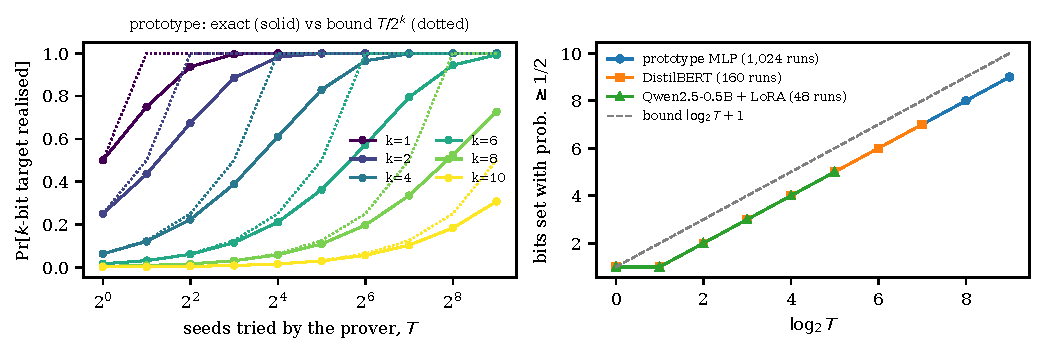
\includegraphics[width=0.8\textwidth]{fig/e3_grinding.pdf}
\caption{Seed grinding through a seed-accepting binding check. Left: prototype
(\EthreeN{} runs), exact probability of realising a random $k$-bit target (solid) and the
bound $T/2^k$ of Theorem~\ref{thm:grind} (dotted). Right: bits set with probability $\ge1/2$
for the prototype, DistilBERT (G1, \GOneN{} runs) and Qwen2.5-0.5B~+~LoRA (G4, \GFourN{}
runs); the three curves coincide where they overlap.}\label{fig:e3}
\end{figure*}

\subsection{Language-model scale (GPU)}

The prototype model is small. To check that binding by replay, grinding and detector
recall behave the same way for language models, we ran four experiments (G1--G4) on one consumer
GPU (NVIDIA \GPUname, 8\,GB; PyTorch \GPUtorch, CUDA \GPUcuda, Transformers \GPUtf) using
SST-2~\cite{socher2013sst}. The models were DistilBERT (\texttt{distilbert-base-uncased},
full fine-tuning) and Qwen2.5-0.5B with LoRA~\cite{hu2022lora} (rank 8 on the query and
value projections, sequence-classification head). Training ran in bf16 autocast, one
epoch, maximum length 64. A fifth experiment (G5) ran on a second machine, described below.

\paragraph{G2: exact replay}
Each configuration was trained three times from the same seed on 1,000 examples, both with
PyTorch's deterministic-algorithms mode and with default kernels (Table~\ref{tab:g2}). In
all four configurations the three runs produced bit-identical weights. Re-execution is
therefore a valid \textsf{BindFix}/\textsf{BindGrind} realisation for fine-tuning at this
scale on fixed hardware and software. Across machines it is not: G5 below re-executed nine
G3 runs on a second GPU with newer software, and none reproduced.

\begin{table}[t]
\centering\scriptsize
\caption{G2: replay of fine-tuning on one GPU (3 runs per row, same seed and data).}\label{tab:g2}
\resizebox{\columnwidth}{!}{\begin{tabular}{@{}llrcrr@{}}
\toprule
Model & kernels & trainable params & distinct hashes & max $|\Delta w|$ & train s\\
\midrule
\csname @@input\endcsname gen/tab_g2_rows.tex
\bottomrule
\end{tabular}}
\end{table}

\paragraph{G3: authorised-source poison at LLM scale}
An authorised source contributes $n$ dirty-label backdoor examples (negative sentences with
the trigger ``cf'' inserted, relabelled positive) to an 8,000-example committed set. Every
example carries a valid content-addressed Ed25519 receipt, so every provenance check
passes. We then measure the backdoor's attack success on triggered negative validation
sentences, and the recall of spectral signatures on DistilBERT's final-layer
\texttt{[CLS]} representation, flagging $1.5\varepsilon n_c$ items per class with
$\varepsilon=0.05$ (Table~\ref{tab:g3}).

\paragraph{Statistical treatment}
The replication unit is the training run (seed). Validation sentences within one run are not
independent replications of the model, so we report run-level values. For each run we give a
Wilson 95\% interval for its proportions, over $n=428$ triggered negative validation sentences
(attack success) and $n$ poisoned items (recall). We also give the attack success minus that of
the clean model with the same seed (\emph{baseline-adjusted}). With three seeds per condition
we report descriptive statistics only. A significance test over three runs would carry little
information (Table~\ref{tab:g3stats}).

The two curves cross. At 0.25--1\% poison, the detector finds 68--83\% of poisoned items on
average, but the backdoor has not taken hold after one epoch: mean baseline-adjusted attack
success stays between $-1$ and $+4$ points, with one run reaching $+9$ points at 1\%. At 2\%, the backdoor is effective in all three
runs, but unequally: baseline-adjusted attack success is $+\GthreeAdjHigh$ points on average,
ranging from $+\GthreeAdjHighMin$ to $+\GthreeAdjHighMax$. Mean recall falls to 25\%, with
wide per-run intervals.

Precision is the practical problem. The flag budget ($1.5\varepsilon n_c$ per class) sends
about \GthreeFPHigh{} clean examples per run to review at 2\% poison
(\GthreeFPRHigh\% of clean items). Only \GthreePrecHigh\% of flagged items are poisoned at 2\%,
and \GthreePrecLow\% at 0.25\%. A reviewer who inspects every flag therefore reads hundreds of
clean sentences per run, and still misses most of the poison where it matters. These are
results for one detector, one model and one trigger. They do not characterise poisoning
detection in general.

An auditor who holds a valid provenance record for this model holds no evidence about the
backdoor. This is Theorem~\ref{thm:content} measured on a pretrained transformer.
G5 below adds two detectors, a clean-data baseline and a higher poison level at GPU scale.

\begin{table}[t]
\centering\scriptsize
\caption{G3 summary: authorised-source backdoor poison, DistilBERT on SST-2 (3 seeds; mean
and range). Attack success over $n=428$ triggered negative sentences per run; clean accuracy
over $n=872$.}\label{tab:g3}
\resizebox{\columnwidth}{!}{\begin{tabular}{@{}rrclllr@{}}
\toprule
$n$ & rate & receipts & attack succ. & clean acc. & recall\phantom{x} & flagged\\
\midrule
\csname @@input\endcsname gen/tab_g3_rows.tex
\bottomrule
\end{tabular}}
\end{table}

\begin{table*}[t]
\centering\scriptsize
\caption{G3 per run (seeds 1, 2, 3). Attack success and recall in \% with Wilson 95\%
intervals; attack success over $n=428$ triggered negative sentences, recall over the $n$ poisoned
items. ``Adj.'': mean attack success minus the clean model's with the same seed, in percentage
points. FP: clean items flagged, mean over runs (rate over 8,000 clean items).}\label{tab:g3stats}
\begin{tabular}{@{}rp{6.2cm}rp{5.2cm}r@{}}
\toprule
$n$ & attack success per run [95\% CI] & adj. & recall per run [95\% CI] & FP (rate)\\
\midrule
\csname @@input\endcsname gen/tab_g3_stats_rows.tex
\bottomrule
\end{tabular}
\end{table*}

\paragraph{G5: three detectors and a second machine}
We added G5 in revision. It repeats the G3 protocol unchanged (same code, data, trigger,
seeds and training settings) at 0, 80, 160 and 320 poisoned items (0--3.8\%), and scores every
committed item with the three detectors of E2d, using the E2d flagging rules fixed before
the run. Unlike E2d, the detectors are applied to the trained model itself, as in G3. Because
the RTX~3070 machine was not available, G5 ran on a second machine: an NVIDIA \GFiveGPU{}
(\GFiveMem\,GB; PyTorch \GFiveTorch, CUDA \GFiveCuda, Python \GFivePy, Transformers \GFiveTf),
with deterministic kernels throughout, \GFiveTrainS\,s of training per run and at most
\GFivePeakGB\,GB of GPU memory. All \GFiveRuns{} runs completed, and \GFiveChecksOK{} of
\GFiveChecks{} automatic validity checks passed. The two that failed are the expected device
and the exact replay of G3, discussed next. Table~\ref{tab:g5} gives pooled recall and the
threshold-free AUROC within the target class, computed from the saved per-item scores.

\emph{Replay across machines.} Nine G5 runs (0, 80 and 160 poisoned items, seeds 1--3) are
exact re-executions of G3 runs. None reproduced G3's attack success, and \GFiveReplayAccEq{}
of \GFiveReplayN{} reproduced its clean accuracy. Below 2\% poison, attack success differed
by at most \GFiveReplayLowMaxDiff{} points; at 2\% it differed by up to \GFiveReplayMaxDiff{}
points for the same seed. GPU architecture and library versions changed together, so we
cannot attribute the difference to either. The practical consequence is clear: an auditor who
re-executes on a different stack does not obtain the trainer's model, so re-execution binding
needs a pinned hardware and software stack or a tolerance, and a tolerance enlarges
$\mathcal A_C$ (Theorem~\ref{thm:grind}).

\emph{Detection.} The qualitative results of G3 recur on the second machine. At 1\% poison
the backdoor has not taken hold, and the poison is easy to separate: AUROC
\GFiveSpecAucLow{} (spectral) and \GFiveLossAucLow{} (loss), with \GFiveSpecRecLow\% and
\GFiveLossRecLow\% recall within the flag budget, but only \GFiveSpecPrecLow\% precision. At
3.8\% the backdoor succeeds in every run (attack success at least \GFiveAsrHighMin\%), and
both detectors flag \GFiveRecHighTP{} of \GFiveHighN{} poisoned items; their AUROC
(\GFiveSpecAucHigh{} and \GFiveLossAucHigh) is at or below chance, so the poison looks
\emph{more} typical than clean data. Over the nine poisoned runs, recall falls as attack
success rises (Spearman $\rho=\GFiveRhoSpec$ for both; descriptive, since poison level drives
both; Fig.~\ref{fig:g5}). Activation clustering flagged a cluster in every run, including all three clean runs,
where it flagged \GFiveACCleanMin--\GFiveACCleanMax\% of clean items; its precision never
exceeded \GFiveACPrecMax\%. With this configuration it is not a usable detector here. These
results extend G3 to more detectors, a clean baseline and a higher poison rate; they use the
same model, data and trigger, so they say nothing about other models or attacks.

\begin{figure}[t]
\centering
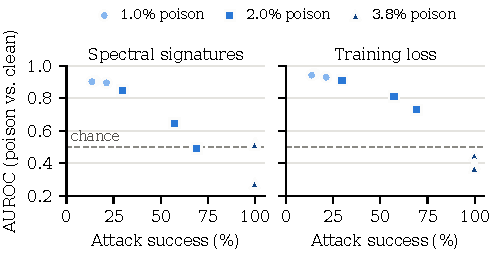
\includegraphics[width=\columnwidth]{fig/g5_detection.pdf}
\caption{G5: separability of poisoned from clean items (AUROC within the target class) against
the backdoor's attack success, one point per run. Detection is good only while the attack
fails; once the backdoor works in every run (3.8\% poison), both detectors are at or below
chance.}\label{fig:g5}
\end{figure}

\begin{table*}[t]
\centering\scriptsize
\caption{G5: three detectors on DistilBERT/SST-2 with authorised-source poison, run on a
second machine (\GFiveGPU; 3 seeds per row). Attack success: mean (range) over $n=428$
triggered negative sentences per run; clean accuracy over $n=872$. Recall: poisoned items
flagged out of all poisoned items over the 3 runs, flag budget $1.5\varepsilon n_c$ per class
($\varepsilon=0.05$, about 7.5\% of clean items by construction). AUROC: within the target
class, mean (range) over runs. Activation clustering: mean share of clean items flagged
(runs that flagged anything).}\label{tab:g5}
\begin{tabular}{@{}rrllllllr@{}}
\toprule
& & & & \multicolumn{2}{c}{spectral signatures} & \multicolumn{2}{c}{training loss} & act.\ clustering\\
$n$ & rate & attack succ.\ \% & clean acc.\ \% & recall & AUROC & recall & AUROC & clean FP\\
\midrule
\csname @@input\endcsname gen/tab_g5_rows.tex
\bottomrule
\end{tabular}
\end{table*}

\paragraph{G1 and G4: grinding at LLM scale}
We repeated E3 with \GOneN{} DistilBERT fine-tuning runs on a fixed 8,000-example committed set
(G1; \GOneTrainS\,s each; held-out accuracy $\GOneAcc\%\pm\GOneAccSd$; all \GOneDistinct{}
weight hashes distinct), and with \GFourN{} Qwen2.5-0.5B~+~LoRA runs on 2,000 examples
(G4; \GFourTrainS\,s each; accuracy $\GFourAcc\%\pm\GFourAccSd$). The probes, the disjoint
selection and evaluation seeds, and the exact analysis are the same as in E3. On the
selection seeds, \GOneSens\% (DistilBERT) and \GFourSens\% (Qwen~+~LoRA) of the 872 SST-2
validation sentences changed label across seeds.

The bits set with probability at least $1/2$ were exactly $\log_2T$ at every
$T\ge2$ for both models: \GOneBits{} bits at $T=\GOneTmax$ for DistilBERT and \GFourBits{}
bits at $T=\GFourTmax$ for Qwen~+~LoRA (Fig.~\ref{fig:e3}, right). This is the same curve as the
small prototype. In this setting, the channel's capacity is set by the number of training runs
the prover can afford, not by the model. Again the ground models were of ordinary quality:
\GOneChosenAcc\% against \GOneAllAcc\% for DistilBERT ($k=\GOneStK$, $T=\GOneStT$), and
\GFourChosenAcc\% against \GFourAllAcc\% for Qwen~+~LoRA ($k=\GFourStK$, $T=\GFourStT$).
At the measured training times, setting 7 chosen bits of a DistilBERT fine-tune takes under an hour
on a laptop GPU.

\subsection{Cost of record-level mechanisms (E4)}

\begin{table}[t]
\centering\scriptsize
\caption{Cost of record-level mechanisms on one CPU core (1\,KiB items). Per-item costs in
$\mu$s. Merkle root over all items in ms.}\label{tab:e4}
\setlength{\tabcolsep}{4.5pt}\begin{tabular}{@{}rrrrrrr@{}}
\toprule
items & hash & sign rcpt & verify rcpt & root (ms) & proof len & receipts (MB)\\
\midrule
\csname @@input\endcsname gen/tab_e4_rows.tex 
\bottomrule
\end{tabular}
\end{table}

Table~\ref{tab:e4} shows that hashing, receipts and commitments cost microseconds per item
and scale linearly. At the measured rate, verifying receipts for a corpus of $10^9$ documents would take about
\EfourVerifyHours{} core-hours, and the work is trivially parallel. The dominant cost of any
configuration that includes binding is binding itself. Exact re-execution doubles training,
and proof systems cost much more~\cite{abbaszadeh2024zkpot,liao2026verilora}.

\subsection{Published systems through the model (E1)}

Table~\ref{tab:e1} maps published systems to the model and reads off the goals they support.
The mapping uses each paper's own description of its mechanisms and trust assumptions. For
Atlas and VAMP we read the threat-model sections. For the others the mapping is from the
abstract and is marked as such.

\begin{table*}[t]
\centering\scriptsize
\caption{Published systems mapped to the model. ``Profile'' is the closest adversary profile
implied by the paper's threat model. Mechanisms marked $\tau$ are realised by trusted
hardware and are lost under \textsf{AdvTEE}.}\label{tab:e1}
\begin{tabular}{@{}p{2.3cm}p{3.6cm}p{2.1cm}p{4.6cm}p{3.6cm}@{}}
\toprule
System & Mechanisms (as described) & Profile & Goals supported per the model & Remark\\
\midrule
Atlas~\cite{spoczynski2025atlas} (threat model read) & TEE attestation of every transformation and its inputs; transparency log & MLaaS provider, hubs, producers untrusted $\approx$ full & With CPU-only TEEs and GPU training outside them (the paper's own limitation): $G_{\mathrm{compl}}$ only. With attested training (Bind under $\tau$): $G_{\mathrm{bind}}$, $G_{\mathrm{auth}}$ via AC+AT+$\beta$ & Dataset benignity out of scope, consistent with Thm.~\ref{thm:content}\\
Laminator~\cite{duddu2025laminator} (abstract) & Hardware-attested property cards for data, training, inference & full & Attested claims only under $\tau$; under full+tee none remain & No content claim beyond attested properties\\
VAMP~\cite{stokes2021prevent} (threat model read) & Signed manifests over datasets, software, models (WitSrc) & Infrastructure trusted $\approx$ trans-only & $G_{\mathrm{auth}}$ for filter-only pipelines; no $G_{\mathrm{zero}}$ & Title claims poisoning \emph{prevention}; holds for unauthorised modification only (Thm.~\ref{thm:content}.1)\\
PoL~\cite{jia2021pol} & Spot-check re-execution with tolerance, prover-chosen randomness & exec-only & $G_{\mathrm{bind}}$ up to spoofing~\cite{fang2023pol}; not $G_{\mathrm{noinf}}$ (BindGrind) & Tolerance enlarges the grinding set (Thm.~\ref{thm:grind})\\
VeriLoRA~\cite{liao2026verilora} (protocol sections read) & ZK proof of every LoRA step (forward, backward, update); initial weights committed as part of the witness & exec-only & $G_{\mathrm{bind}}$ as \textsf{BindGrind}: the paper does not fix mini-batch sampling or initialisation randomness by the verifier, so not $G_{\mathrm{noinf}}$; no dataset commitment is described, so binding to a record needs one; no lineage without WitSrc or attestation & Combine with a beacon-derived seed and data commitment to obtain \textsf{BindFix}\\
Kaizen zkPoT~\cite{abbaszadeh2024zkpot} (protocol sections read) & ZK proof of every training iteration over a Merkle-committed dataset; prover commits the initial weights; batch order from a public pseudorandom permutation key & exec-only & $G_{\mathrm{bind}}$ as \textsf{BindGrind}: the prover commits its own initial weights, the protocol does not require the permutation key to be fixed by the verifier after the data commitment, and the number of proved iterations need not be fixed in advance, so not $G_{\mathrm{noinf}}$; no lineage without WitSrc or attestation & Seed rejection sampling against zkPoTs demonstrated by~\cite{tan2025zkpot}\\
Optimum-vicinity zkPoT~\cite{tan2025zkpot} (full text read) & ZK proof that the released model is within $\epsilon$ of the optimum of an $L_2$-regularised convex loss on the committed data & exec-only & $G_{\mathrm{bind}}$ with $\mathcal A_C$ an $\epsilon$-ball, independent of training randomness; influence bounded geometrically rather than by $T$ & Logistic regression and SVMs; no lineage or content claim\\
AuditableLLM~\cite{li2025auditablellm} (abstract) & Hash-chained audit trail of updates & exec-only & Store integrity ($P_1$) only; no pipeline goal & ``Verifiable integrity'' is of the log, not of the training\\
Mehammed et al.~\cite{mehammed2025fl} (abstract) & Permissioned ledger, update audit, zk-SNARK of client summaries & full (clients untrusted) & $P_1,P_2,P_8$; no binding of client training, so no pipeline goal & Ledger contributes $P_8$ (Prop.~\ref{prop:ledger})\\
\bottomrule
\end{tabular}
\end{table*}

The pattern is consistent. Systems that state a narrow threat model (Atlas and VAMP, which
trust the verification or training infrastructure) make claims that the model supports
within that model. The model's value is that it says what changes when the trust assumption
does not hold. Claims phrased as preventing poisoning, or as verifiable integrity of
training, hold only for the narrower properties the model identifies.

% ---------------------------------------------------------------
\section{Literature Search Method}\label{sec:lit}
% ---------------------------------------------------------------

The systematisation in Section~\ref{sec:sok} rests on a structured search. We report it
in PRISMA~2020 terms~\cite{page2021prisma} and state plainly which stages are incomplete.

\paragraph{Search}
On 25~October~2026 we ran 12 query strings against OpenAlex. The strings cover provenance
and lineage capture, ledgers, transparency logs, trusted execution, proofs of learning,
zero-knowledge training proofs, data-use auditing and poisoning defences. We retrieved
the first 25--100 results per string (24 result pages in total, depth by string as
recorded in the artefact). This produced 594 records. A version-aware deduplication kept
the peer-reviewed version of each work and recorded all its DOIs, which removed 43
duplicates.

\paragraph{Eligibility}
Inclusion required (I1) an ML or AI training pipeline, (I2) a mechanism for provenance,
integrity or verification of training data or training computation, and (I3) peer review.
Exclusion codes covered: no ML context (E1); inference-output provenance only (E2);
document types outside the protocol (E3); poisoning work without a provenance or
verification component (E5); and preprint-only works (E7). E7 works were kept in a
separate positioning list and are not cited as evidence.

\paragraph{Screening}
A rule-based pre-screen excluded 248 of 551 records: 135 preprint-only, 90 without ML or
provenance terms, and 23 by document type. An audit of 92 rule exclusions by title found
2 false exclusions, which were restored. Title-and-abstract screening of the remaining 303
records was carried out by an AI assistant (Claude) applying the written protocol. Every
decision is logged with a reason code and labelled as an AI decision requiring human
verification. It excluded 154 records and passed 149 (55 marked \emph{unsure}). Nine further
records came from citation chasing. That leaves 158 records for full-text assessment.

\paragraph{Status and limits}
\pending{Full-text screening of the 158 records, a human second screener with reported
agreement ($\kappa$) on at least a 20\% sample, and searches of Scopus, Web of Science,
IEEE~Xplore and the ACM Digital Library are not yet complete. Until they are, the search
is a structured mapping, not a systematic review.} A known-item check found 8 of 17 seed
papers that the authors had identified beforehand. The misses include Atlas and Sigstore,
which is why the database searches above are required before submission. The screening log,
queries and raw result pages are part of the artefact.

% ---------------------------------------------------------------
\section{Discussion}\label{sec:discussion}
% ---------------------------------------------------------------

\subsection{What an auditor may conclude}

\begin{figure}[t]
\centering
\resizebox{\columnwidth}{!}{\input{fig/fig_auditor}}
\caption{Four questions an auditor should answer before accepting a claim about a released
model, and what the theorems and experiments say for each answer.}
\label{fig:auditor}
\end{figure}

Table~\ref{tab:minimal} can be read as a checklist, and Fig.~\ref{fig:auditor} condenses it
into four questions. Before accepting a claim about a
released model, an auditor should establish three things:
\begin{enumerate}
\item Who is trusted: which profile applies.
\item Which mechanisms were actually deployed and verified.
\item Which goal the claim corresponds to.
\end{enumerate}
Two examples show how this works.

A cloud provider's attested data pipeline without binding (\textsf{AttCap}, \textsf{AttTrans}
under the full adversary) supports no claim about the released model. It does support the
record-level claim $G_{\mathrm{compl}}$.

A signed-manifest scheme with a trusted training infrastructure (the trans-only or cap-only
profiles) does support lineage for filter-only pipelines, but not the absence of poison.

\subsection{Answers to five design questions}

\paragraph{Binding}
Binding is required whenever the trainer is not trusted, and no amount of witnessing or
attestation of earlier stages substitutes for it (Theorem~\ref{thm:bind}). If binding is
used, its randomness must be fixed after commitment (Theorems~\ref{thm:noinf}
and~\ref{thm:grind}). Exact re-execution is a valid binding only where training is
bit-reproducible. Section~\ref{sec:eval} measures when it is.

\paragraph{Witnessing}
Source receipts must be content-addressed (split view, Section~\ref{sec:eval}). Source
witnessing and input witnessing answer different questions, lineage and completeness. Each
fails under collusion, so witnesses should be organisationally independent of the operator
they observe.

\paragraph{Synthetic data}
Generative stages need an attested transform even on the witness route, and stage types
must be declared and authenticated (Corollary~\ref{cor:launder}). Lineage of synthetic data
is recursive: the generator is itself a model whose provenance matters. Our model treats it
as an authorised but possibly poisoned source (\textsf{AdvGen}).

\paragraph{Blockchain versus transparency logs}
For every goal we study, a witnessed transparency log is sufficient as the record store.
A ledger adds inclusion liveness (Proposition~\ref{prop:ledger}). We find no support for
the claim that a blockchain makes training records complete or truthful. Those properties
are decided upstream of the store.

\paragraph{Poisoning}
Provenance cannot certify that a model is poison-free (Theorem~\ref{thm:content}). It can
make a detector's verdict \emph{transfer} to the released model, which is what binding and
completeness contribute. The resulting claim is only as strong as the detector's recall.
In our experiments, recall was weakest exactly where the poison worked. The prototype's detector flagged at most a quarter of the planted items. On DistilBERT, recall fell from 68--83\% at the lower, ineffective poison rates to 25\% at the 2\% rate where the backdoor took hold (Section~\ref{sec:eval}). Any
certification scheme that reports provenance without detector recall overstates its
assurance.

\subsection{Open problems}

\begin{enumerate}
\item \emph{Binding at pre-training scale.} Zero-knowledge binding now reaches LoRA
  fine-tuning~\cite{liao2026verilora}, but not full pre-training. Exact re-execution
  doubles the cost and requires determinism. Spot-check proofs of learning admit spoofing
  under tolerance~\cite{fang2023pol}.
\item \emph{Tolerance as a grinding channel.} Theorem~\ref{thm:grind} bounds influence by the
  number of accepted trajectories. For tolerance-based verifiers that number is not
  characterised. Optimum vicinity~\cite{tan2025zkpot} closes the channel for convex
  objectives; for non-convex LLM training it remains open.
\item \emph{Attested accelerators.} The attestation routes assume that the relevant stages run
  in TEEs. Atlas notes that GPUs lack equivalent protection~\cite{spoczynski2025atlas}.
\item \emph{Detector guarantees.} $G_{\mathrm{content}}$ is parameterised by recall. Certified
  recall bounds for poisoning detectors at LLM scale are lacking.
\item \emph{Confidential verifiability ($P_7$).} All our mechanisms reveal the record to the
  auditor. Combining them with confidentiality of training data is open.
\item \emph{Composition across model generations.} Fine-tuning chains and synthetic data make
  provenance recursive. The model covers one training run.
\end{enumerate}

\subsection{Limitations}

\paragraph{Model}
The model has five abstractions:
\begin{itemize}
\item Items are atomic and content-identified.
\item Each mechanism is all-or-nothing.
\item A single training run is modelled.
\item Detectors are abstracted to an examined set and a miss set, with no budget or base
  rate.
\item Correlated compromise is captured \emph{across} trust anchors (any subset of
  capabilities), but not \emph{within} a mechanism class, such as one corrupt witness among
  several.
\end{itemize}
Table~\ref{tab:scope} lists which training practices fall inside the abstraction. The
model's results are exact for the model only. Their relevance to real systems rests on the
validation in Section~\ref{sec:eval}.

\paragraph{Prototype}
The prototype trains a small bag-of-words network on 2,000 reviews. It simulates trusted
execution with key isolation rather than real enclaves, so it validates the logic of
attestation-based checks, not any hardware. It compares three detectors on one small model. Poisoning at GPU scale was
measured on one model (DistilBERT), one dirty-label trigger and three seeds per condition,
with one detector in G3 and three in G5, so it is reported descriptively. G5 ran on a second,
smaller GPU because the first was unavailable; its qualitative results match G3, but its runs
did not replay G3's bit for bit. Bit-exact replay therefore holds on a fixed stack only, and
we changed GPU and library versions together, so we cannot say which change breaks it. The
GPU experiments cover fine-tuning, not pre-training.
Their seed counts (160 and 48) limit the largest $T$ we could test to 128 and 32.

\paragraph{Literature}
The literature search used one database, title-and-abstract screening was performed by an
AI assistant, and full-text assessment is pending (Section~\ref{sec:lit}). The case-study
mapping relies partly on abstracts.

\paragraph{Proofs}
The proofs are by hand. They are backed by two independent exhaustive decision procedures
for the six profiles, and by a third, vectorised checker over all 128 adversary subsets. They
are not mechanised in a proof assistant. Proposition~\ref{prop:ledger} and the composition
remark of Section~\ref{sec:scope} are argued, not proved.


\section{Artefact, Data, Ethics and AI-Use Statement}\label{sec:artefact}
\paragraph{Artefact}
The artefact contains:
\begin{itemize}
\item the Alloy models, the sweep, the independent checker, the adversary-lattice checker and
  their raw outputs;
\item the prototype and every experiment script with raw and processed results;
\item the GPU kit with its logs;
\item the G5 kit, its logs and per-item detector scores;
\item the literature-search queries, raw result pages and screening log;
\item SHA-256 manifests and a reproducibility guide that regenerates every table and figure.
\end{itemize}
The artefact is archived on Zenodo, version~1.1:
\url{https://doi.org/10.5281/zenodo.24420107} (all versions:
\url{https://doi.org/10.5281/zenodo.24317966}). Code is released under the MIT licence and
results, data and documentation under CC~BY~4.0. A working copy is maintained at
\url{https://github.com/waqas6755/what-can-provenance-prove}. The archive holds a reproducibility
guide that maps each table and figure to the script and raw file that produce it, and SHA-256
checksums of its files.

\paragraph{Data, models and licences}
The prototype uses the polarity dataset v2.0~\cite{pang2004sentimental}, as distributed by
NLTK. The GPU experiments use SST-2~\cite{socher2013sst} from the GLUE distribution, with
\texttt{distilbert-base-uncased} and \texttt{Qwen/Qwen2.5-0.5B} from the Hugging Face Hub. No
personal data is processed. Both models are released under the Apache~2.0 licence. Neither the
polarity dataset nor the Stanford Sentiment Treebank states a licence: the polarity dataset's
distribution page asks users to cite its version number, and the GLUE distribution refers users to
the licence of each source dataset. We use both datasets unmodified, for research only, and do not
redistribute them; the artefact gives download instructions instead.

\paragraph{Dual use and disclosure}
The attacks we implement (split-view delivery, laundering, seed grinding, authorised-source
backdoors) are either already published or follow directly from the model. They are run only
against our own prototype and public models. The grinding result points to a simple
mitigation, a beacon-fixed seed, which we recommend to builders of proof-of-training systems.
No third-party system was attacked.

\paragraph{AI assistance}
An AI assistant (Claude, Anthropic) was used to:
\begin{itemize}
\item write experiment and analysis code;
\item run the model checker and the experiments in the cloud environment;
\item draft and revise text;
\item perform title-and-abstract screening.
\end{itemize}
The AI screening decisions are labelled as such in the released log. They have not been
verified by a human screener, and they are not reported as independent human screening. The
authors are responsible for verifying the code, results and proofs, and for all claims.
\pending{State which verification the authors have personally carried out.} \pending{Check this statement against the journal's current AI-use policy before
submission.}

\section{Conclusion}
We separate the conclusions by the kind of evidence behind them.

\paragraph{Proved within the model}
\begin{itemize}
\item Computation binding is necessary exactly when the trainer is untrusted.
\item Lineage has two routes with disjoint trust anchors.
\item Generative pipelines need authenticated stage types.
\item A seed-accepting binding check leaks at most $\log_2T$ bits for $T$ evaluated accepted
  outputs.
\item No mechanism set certifies the absence of poison; the strongest claim is conditional on
  a detector.
\item Attested capture and input witnessing are interchangeable for record completeness.
\end{itemize}
These statements hold for every subset of adversary capabilities. They are exact for the
abstract single-run model of Section~\ref{sec:model}, within the scope of
Table~\ref{tab:scope}.

\paragraph{Observed in our experiments}
\begin{itemize}
\item A prototype with real cryptography and simulated trusted execution matched the model
  on all 9,216 instances.
\item Seed grinding reached $\log_2T$ bits on a small model, on DistilBERT and on Qwen
  2.5-0.5B~+~LoRA.
\item Fine-tuning replayed bit for bit on one machine, but not on a second machine with a
  different GPU and newer libraries.
\item One spectral-signature detector lost most of its recall exactly where an
  authorised-source backdoor became effective, at low precision.
\item On the prototype, three detectors, including a loss score and activation clustering,
  showed the same pattern or found nothing.
\item At GPU scale, spectral and loss detectors separated poison well at 1\% poison and fell
  to chance at 3.8\%, where the backdoor always worked; activation clustering flagged about a
  quarter of clean data even with no poison.
\end{itemize}

\paragraph{From the literature}
The surveyed systems make claims that hold within their own trust assumptions. Claims of
poisoning prevention, or of verifiable integrity of training, hold only for the narrower
properties identified in Table~\ref{tab:e1}. This conclusion rests on a structured mapping,
not yet a systematic review (Section~\ref{sec:lit}).

\paragraph{Design rules and future work}
\begin{itemize}
\item Bind the computation whenever the trainer is untrusted, with randomness fixed after
  commitment.
\item Use content-addressed receipts and authenticated stage types.
\item Diversify trust anchors.
\item Report detector recall and precision alongside any content claim.
\item Use a ledger only where censorship-resistant inclusion is itself a requirement.
\end{itemize}
Future work includes binding at pre-training scale, replay across hardware stacks (which
failed in our one cross-machine test), multi-stage and
multi-parent model lineages, real enclave deployments, and detectors with guaranteed recall.

\bibliographystyle{IEEEtran}
\bibliography{refs}

\ifproofsinpaper
\appendices
% ---------------------------------------------------------------
\section{Proofs}\label{app:proofs}
% ---------------------------------------------------------------
\input{app_proofs_body}

\fi

\end{document}
"
\newif\ifproofsinpaper\ifdefined\withproofs\proofsinpapertrue\fi
\newcommand{\proofsloc}{\ifproofsinpaper Appendix~\ref{app:proofs}\else Supplementary Section~S10\fi}
\newcommand{\pending}[1]{{\color{red!70!black}[\textbf{PENDING:} #1]}}

\newcommand{\Ehonestfull}{yes}
\newcommand{\Ehonestfullwit}{yes}
\newcommand{\Ehonestfulltee}{yes}
\newcommand{\Ehonestcaponly}{yes}
\newcommand{\Ehonestexeconly}{yes}
\newcommand{\Ehonesttransonly}{yes}
\newcommand{\Etwoinst}{9{,}216}
\newcommand{\Etwoholds}{4{,}776}
\newcommand{\Etwounsound}{0}
\newcommand{\Etwofails}{4{,}440}
\newcommand{\Etworeal}{4{,}440}
\newcommand{\Etworuns}{3{,}498{,}118}
\newcommand{\Etwoacc}{656{,}798}
\newcommand{\SVtrials}{200}
\newcommand{\SVname}{200}
\newcommand{\SVcontent}{0}
\newcommand{\CENheads}{20}
\newcommand{\CENcos}{20}
\newcommand{\EthreeN}{1{,}024}
\newcommand{\EthreeSel}{128}
\newcommand{\EthreeEval}{896}
\newcommand{\EthreeAcc}{79.0}
\newcommand{\EthreeAccSd}{1.4}
\newcommand{\EthreeSens}{24.8}
\newcommand{\EthreeReplay}{yes}
\newcommand{\EthreeBitsMax}{9}
\newcommand{\EthreeTMax}{512}
\newcommand{\EthreeTrainS}{0.22}
\newcommand{\EthreeChosenAcc}{79.0}
\newcommand{\EthreeAllAcc}{79.0}
\newcommand{\EfourVerifyHours}{32}
\newcommand{\MCcompared}{9{,}216}
\newcommand{\MCagree}{9{,}216}
\newcommand{\GPUname}{RTX 3070 Laptop GPU}
\newcommand{\GPUtorch}{2.6.0}
\newcommand{\GPUcuda}{12.4}
\newcommand{\GPUtf}{5.22.1}
\newcommand{\GOneN}{160}
\newcommand{\GOneTmax}{128}
\newcommand{\GOneBits}{7}
\newcommand{\GOneAcc}{87.5}
\newcommand{\GOneAccSd}{0.6}
\newcommand{\GOneSens}{14.8}
\newcommand{\GOneTrainS}{15}
\newcommand{\GOneBitsList}{$T{=}1$: 1, $T{=}2$: 1, $T{=}4$: 2, $T{=}8$: 3, $T{=}16$: 4, $T{=}32$: 5, $T{=}64$: 6, $T{=}128$: 7}
\newcommand{\GOneDistinct}{160}
\newcommand{\GFourN}{48}
\newcommand{\GFourTmax}{32}
\newcommand{\GFourBits}{5}
\newcommand{\GFourAcc}{76.8}
\newcommand{\GFourAccSd}{5.5}
\newcommand{\GFourSens}{74.4}
\newcommand{\GFourTrainS}{27}
\newcommand{\GFourBitsList}{$T{=}1$: 1, $T{=}2$: 1, $T{=}4$: 2, $T{=}8$: 3, $T{=}16$: 4, $T{=}32$: 5}
\newcommand{\GOneChosenAcc}{87.5}
\newcommand{\GOneAllAcc}{87.5}
\newcommand{\GOneStK}{6}
\newcommand{\GOneStT}{64}
\newcommand{\GFourChosenAcc}{77.0}
\newcommand{\GFourAllAcc}{76.8}
\newcommand{\GFourStK}{4}
\newcommand{\GFourStT}{16}

\newcommand{\RevEtwoRuns}{3{,}498{,}118}
\newcommand{\RevEtwoAcc}{656{,}798}
\newcommand{\GthreeAdjHigh}{50.9}
\newcommand{\GthreeAdjHighMin}{20.1}
\newcommand{\GthreeAdjHighMax}{74.5}
\newcommand{\GthreeFPHigh}{574}
\newcommand{\GthreePrecHigh}{6.4}
\newcommand{\GthreePrecLow}{2.7}
\newcommand{\GthreeFPRHigh}{7.2}

\newcommand{\GFiveGPU}{GTX 1650}
\newcommand{\GFiveMem}{4}
\newcommand{\GFiveTorch}{2.11.0}
\newcommand{\GFiveCuda}{12.8}
\newcommand{\GFivePy}{3.14.10}
\newcommand{\GFiveTf}{5.22.1}
\newcommand{\GFiveRuns}{12}
\newcommand{\GFiveTrainS}{104}
\newcommand{\GFivePeakGB}{1.4}
\newcommand{\GFiveChecksOK}{64}
\newcommand{\GFiveChecks}{66}
\newcommand{\GFiveReplayN}{9}
\newcommand{\GFiveReplayAsrEq}{0}
\newcommand{\GFiveReplayAccEq}{1}
\newcommand{\GFiveReplayMaxDiff}{16.6}
\newcommand{\GFiveReplayLowMaxDiff}{1.9}
\newcommand{\GFiveRhoSpec}{-0.97}
\newcommand{\GFiveRhoLoss}{-0.97}
\newcommand{\GFiveACCleanMin}{19}
\newcommand{\GFiveACCleanMax}{32}
\newcommand{\GFiveACPrecMax}{7.1}
\newcommand{\GFiveSpecAucLow}{0.90}
\newcommand{\GFiveLossAucLow}{0.94}
\newcommand{\GFiveSpecAucHigh}{0.44}
\newcommand{\GFiveLossAucHigh}{0.41}
\newcommand{\GFiveSpecRecLow}{71}
\newcommand{\GFiveLossRecLow}{72}
\newcommand{\GFiveSpecPrecLow}{9.3}
\newcommand{\GFiveRecHighTP}{1}
\newcommand{\GFiveLossRecHighTP}{1}
\newcommand{\GFiveHighN}{960}
\newcommand{\GFiveAsrHighMin}{99.8}

\begin{document}
\title{What Can Provenance Prove?\\ A Systematisation of Assurance for\\ Adversarially Exposed LLM Training Pipelines}
\author{Waqas Ahmed, Ammar Hassan, Attiq Ahmed, and Waseem Iqbal%
\thanks{W.~Ahmed, A.~Hassan and A.~Ahmed are the first, second and third authors. W.~Iqbal is the supervisor and corresponding author. W.~Ahmed, A.~Hassan and A.~Ahmed are with the National University of Sciences and Technology (NUST), Islamabad, Pakistan. W.~Iqbal is with Sultan Qaboos University, Muscat, Oman. \pending{Departments, postal addresses and e-mail addresses.}}}
\markboth{Revised draft (major revision), 21 November 2026 --- not submitted}{Ahmed \MakeLowercase{\textit{et al.}}: What Can Provenance Prove?}
\maketitle

\begin{abstract}
Provenance mechanisms for machine learning (signed data manifests, attested pipelines,
transparency logs, ledgers and proofs of training) are widely proposed as defences for the
integrity of training data. What an auditor may conclude when their checks pass is rarely
stated. We give a precise answer for training-data pipelines of large language models.
We abstract deployed techniques into seven mechanism primitives. We model an adversary
that can corrupt any pipeline stage, collude with witnesses or break trusted hardware, and
we define six assurance goals, from binding a model to its record to excluding poisoned
data. A separability lemma makes the model exactly decidable. We decide all 9,216
(adversary, mechanism set, pipeline type, goal) instances, and two independent procedures
agree on every one. Six theorems follow:
\begin{itemize}
\item Computation binding is necessary exactly when the trainer is untrusted.
\item Lineage has two routes that rest on disjoint trust anchors.
\item Generative pipelines need authenticated stage types.
\item A binding check that accepts a prover-chosen seed leaks up to $\log_2T$ bits of
  influence for $T$ training runs.
\item No mechanism set certifies the absence of poison. The strongest available claim is
  conditional on detector recall.
\item Attested capture and input witnessing are interchangeable for completeness and fail
  under disjoint assumptions.
\end{itemize}
All theorems also hold over every one of the 128 subsets of adversary capabilities. A ledger
adds censorship-resistant inclusion to a witnessed log and nothing else that these goals
need. We test the model on a prototype with real cryptography, simulated trusted execution,
exact training re-execution and an exhaustive adaptive adversary. Across 3.5 million
executions, no accepted execution violated a goal that the model guarantees, and the attacks
realised all 4,440 predicted failures. In a 1,024-run grinding experiment, a prover set
$\log_2T$ chosen bits of model behaviour while passing re-execution, within one bit of our
bound. The same curve holds for DistilBERT and Qwen2.5-0.5B~+~LoRA fine-tuning on a consumer
GPU, where fine-tuning replayed bit for bit on one machine but not on a second one. In the same setting, an
authorised-source backdoor at 2\% poison passed every provenance check and raised attack
success by 20--75 points, while spectral-signature recall averaged 25\% at 6\% precision. With
three detectors, detection fell to chance once the backdoor succeeded in every run. The
results are exact for an abstract single-run model. The experiments cover fine-tuning with one
model family per experiment, not pre-training.
\end{abstract}

\begin{IEEEkeywords}
Data provenance, machine learning security, large language models, data poisoning,
proof of learning, transparency logs, trusted execution, formal methods.
\end{IEEEkeywords}

% ---------------------------------------------------------------
\section{Introduction}\label{sec:intro}
% ---------------------------------------------------------------

Every large language model is the output of a data pipeline. Web crawls, licensed corpora,
human annotations and, more and more, synthetic data from other models are filtered, mixed,
recorded and fed to a training job. Each of these stages is a point where an adversary can
act. Poisoning web-scale training sets is practical~\cite{carlini2024poisoning}. Small
poisoned fractions persist through pre-training into aligned models~\cite{zhang2025persistent}.
Outsourced training can quietly skip or alter steps~\cite{jia2021pol,spoczynski2025atlas}.
In response, a large body of work proposes \emph{provenance} for machine learning: signed
data manifests~\cite{stokes2021prevent}, attested pipelines and transparency
logs~\cite{spoczynski2025atlas,duddu2025laminator}, hash-chained audit
trails~\cite{li2025auditablellm}, blockchain-anchored records~\cite{geren2025blockchain,mehammed2025fl},
and proofs of training~\cite{jia2021pol,abbaszadeh2024zkpot,liao2026verilora}.

These proposals rarely state what an auditor may conclude when the checks pass. Some
claims are too strong. Provenance is said to \emph{prevent} poisoning~\cite{stokes2021prevent},
but an authorised source that supplies poison passes every provenance check. Other claims
are left implicit. A tamper-evident log of a training run says nothing about whether the
released model came from that run unless the computation is bound to the record. Surveys
catalogue the techniques~\cite{geren2025blockchain,lyu2026survey,peng2026zkp}, but none
answers the auditor's question: \emph{given which mechanisms, against which adversary, does
an accepted record prove what?}

Three kinds of assurance are often conflated in this literature, and we keep them apart:
\begin{itemize}
\item \emph{Provenance}: who supplied an item, and what happened to it before training.
\item \emph{Computation verification}: whether the released model was produced from a stated
  record by a stated procedure.
\item \emph{Content assurance}: whether the data is free of poison.
\end{itemize}
The first two are properties of records and computations. The third is a property of data.

\paragraph{Research questions}
\begin{itemize}
\item[\textbf{RQ1}] Which combinations of provenance mechanisms are sufficient, and which are
  minimal, for each assurance goal against each adversary?
\item[\textbf{RQ2}] Which goals can no combination of mechanisms achieve, and what is the
  strongest claim that remains?
\item[\textbf{RQ3}] Do implementations of the mechanisms behave as the model predicts? How
  large are the quantities the model leaves free, such as grinding influence and detector
  recall, in practice?
\end{itemize}

\paragraph{This paper}
We answer these questions for training-data pipelines. Our approach has three parts.

\emph{(1) An assurance model.} We abstract the deployed techniques into seven mechanism
primitives: two kinds of computation binding, source witnessing, input witnessing,
attested capture, attested transform, and an attested content detector. We define seven
adversary capabilities, one per point of trust, including corrupt witnesses and broken
trusted hardware. We define six assurance goals, from ``the record explains the model's
inputs'' to ``no poison was used''.

\emph{(2) An exact characterisation.} A separability lemma shows that every instance of the
model can be decided by reasoning about a single item. We therefore decide all 9,216
(adversary, mechanism set, pipeline type, goal) instances for six named adversary profiles
exactly, with two independent procedures that agree on every one. We then extend the
analysis to all $2^7=128$ subsets of adversary capabilities (196,608 decisions); every
theorem holds over this full lattice. The minimal sufficient mechanism sets
(Table~\ref{tab:minimal}) yield six theorems:
\begin{itemize}
\item Computation binding is necessary exactly when the training executor is untrusted.
\item Lineage has two routes, source witnessing or attested capture-plus-transform, which
  rest on disjoint trust anchors.
\item Generative pipelines need declared and authenticated stage types, or injected data can
  be \emph{laundered} as synthetic.
\item A binding check that accepts a prover-chosen seed leaks influence. We bound it at
  $\log_2T$ bits for $T$ training runs.
\item No mechanism set certifies the absence of poison. The strongest available claim is
  conditional on a detector's recall.
\item Record completeness can be achieved by attestation or by witnessing, which fail under
  disjoint assumptions. This is a formal argument for trust diversity.
\end{itemize}
A ledger adds censorship-resistant inclusion to a witnessed transparency log, and nothing
else that the goals depend on.

\emph{(3) Empirical validation.} The theorems concern a model, so we test whether the model
is faithful. We built a prototype pipeline with real cryptography (Ed25519 receipts, Merkle
commitments, a witnessed transparency log), trusted execution \emph{simulated} by key
isolation, real training on a public sentiment corpus with
exact re-execution, a published backdoor detector~\cite{tran2018spectral}, and an adaptive
adversary that tries every combination of its available attacks. Across all six adversary
profiles and 128 mechanism sets, no execution that the model says is safe violated a goal,
and the attack library realised the model's predicted failures (Section~\ref{sec:eval}). A
grinding experiment with 1,024 training runs shows that a prover can set
$\lfloor\log_2T\rfloor$ chosen bits of model behaviour while passing a re-execution check,
which matches Theorem~\ref{thm:grind} to within one bit. On a single consumer GPU, the same experiments with DistilBERT and Qwen2.5-0.5B~+~LoRA give
three results. Fine-tuning replays bit for bit on fixed hardware, but not on a second GPU
with newer libraries. The grinding curve is
identical: 7 chosen bits for 128 DistilBERT runs. A backdoor delivered at 2\% by an authorised source passes every provenance check.
Across three seeds, it raised attack success by 20 to 75 points over the clean model, while
spectral-signature recall averaged 25\%. On a second machine, three detectors showed the
same pattern: they separate poison well at 1\%, before the backdoor works, and not at all at
3.8\%, where it always works. These GPU results cover fine-tuning with one model family for
poisoning; they do not cover pre-training.

\begin{figure*}[t]
\centering
\resizebox{\textwidth}{!}{% Fig.: method overview (intro), full width
\begin{tikzpicture}[font=\sffamily\scriptsize, >={Stealth[length=1.8mm]},
  bx/.style={draw=black!50, rounded corners=3pt, fill=black!4, text width=28mm, align=flush left,
               minimum height=19mm, execute at begin node={\hyphenpenalty=10000\exhyphenpenalty=10000}, inner sep=2.2pt, anchor=north},
  num/.style={circle, fill=mechblue, text=white, font=\sffamily\tiny\bfseries, inner sep=0.8pt, minimum size=3.6mm},
  fl/.style={->, black!65, line width=0.8pt}]
\def\gap{32.5mm}
\node[bx] (s1) at (0,0) {{\bfseries Systematise}\\[1pt] 594 search records; published mechanisms reduced to \textbf{7 mechanism primitives} (Sec.~II, VI)};
\node[bx] (s2) at (\gap,0) {{\bfseries Model}\\[1pt] pipeline, \textbf{7 adversary capabilities}, \textbf{6 assurance goals}; separability lemma (Sec.~III)};
\node[bx] (s3) at (2*\gap,0) {{\bfseries Decide}\\[1pt] Alloy + independent checker: \textbf{9,216 instances}; all \textbf{128 adversary subsets} (Sec.~IV)};
\node[bx, fill=mechblue!8, draw=mechblue] (s4) at (3*\gap,0) {{\bfseries Prove}\\[1pt] \textbf{6 theorems}: binding, lineage, stage types, grinding ($\log_2T$), content, completeness};
\node[bx] (s5) at (4*\gap,0) {{\bfseries Validate}\\[1pt] prototype (E2--E4, 3.5\,M runs); GPU fine-tuning (G1--G5); published systems mapped (E1) (Sec.~V)};
\node[bx, fill=okgreen!8, draw=okgreen] (s6) at (5*\gap,0) {{\bfseries Advise}\\[1pt] auditor checklist, design rules, open problems (Sec.~VII)};
\foreach \i [count=\j from 2] in {1,...,5} \draw[fl] (s\i.east) -- (s\j.west);
\foreach \i in {1,...,6} \node[num] at (s\i.north west) {\i};
\draw[fl, dashed, mechblue] (s5.south) to[out=-160,in=-20, looseness=0.45] node[below, font=\sffamily\tiny, text=mechblue!80!black]{counterexamples and mismatches refine the model} (s2.south);
\end{tikzpicture}
}
\caption{How the paper answers the auditor's question. Mechanisms from the literature become
primitives of a formal model; the model is decided exactly and yields six theorems; a prototype
and GPU experiments test whether real executions behave as the model predicts. Mismatches found
during validation were used to correct the model (Corollary~\ref{cor:launder}).}
\label{fig:overview}
\end{figure*}

\paragraph{Contributions}
Figure~\ref{fig:overview} summarises the approach.
\begin{itemize}
\item A systematisation of training-data provenance mechanisms as seven primitives, with a
  mapping of published systems to them (Section~\ref{sec:sok}).
\item A formal assurance model with six goals and seven adversary capabilities, together with
  a separability lemma that makes it exactly decidable (Sections~\ref{sec:model}
  and~\ref{sec:results}).
\item A complete characterisation of minimal sufficient mechanism sets for six named
  adversary profiles; six theorems with proofs; and a check of every theorem over all 128
  adversary capability subsets (Section~\ref{sec:results}; proofs in \proofsloc).
\item A prototype and evaluation that test the model's soundness and tightness on real
  executions, a measurement of seed grinding against the bound, and overhead figures
  (Section~\ref{sec:eval}).
\item Design guidance and open problems for auditors, system builders and regulators
  (Section~\ref{sec:discussion}).
\end{itemize}
All models, scripts, raw results and screening logs are archived as an artefact
(Section~\ref{sec:artefact}).

% ---------------------------------------------------------------
\section{Systematisation: Provenance Mechanisms as Primitives}\label{sec:sok}
% ---------------------------------------------------------------

\begin{figure}[t]
\centering
\resizebox{\columnwidth}{!}{% Fig. 1: pipeline stages (grey), mechanism primitives (blue, above), adversary capabilities (orange, below)
\begin{tikzpicture}[font=\sffamily\scriptsize, >={Stealth[length=1.7mm]},
  st/.style={draw=black!55, rounded corners=2pt, fill=black!5, minimum width=15mm,
             minimum height=8.5mm, align=center, inner sep=1pt, font=\sffamily\footnotesize},
  outb/.style={st, fill=white},
  mech/.style={draw=mechblue, fill=mechblue!9, text=mechblue!75!black, rounded corners=2.5pt, minimum height=3.6mm,
               inner sep=1.4pt, font=\sffamily\scriptsize\bfseries},
  adv/.style={draw=advorange, fill=advorange!9, text=advorange!80!black, rounded corners=1pt, minimum height=3.6mm,
              inner sep=1.4pt, font=\sffamily\scriptsize},
  fl/.style={->, black!70, line width=0.65pt}, tie/.style={black!35, line width=0.4pt}]
% stages
\node[st, minimum height=7mm] (src) at (0, 0.55) {Sources \ \textit{D}};
\node[st, minimum height=7mm] (gen) at (0,-0.55) {Generator \ \textit{S}};
\node[st] (tr)  at (2.35,0) {Transform\\\textit{F}};
\node[st] (cap) at (4.45,0) {Capture\\\textit{C}};
\node[st] (ex)  at (6.55,0) {Executor\\\textit{U}};
\node[outb, minimum width=12mm] (mdl) at (8.45,0) {Released\\model};
\node[outb, minimum width=22mm] (store) at (4.45,-2.15) {Record store\\\tiny (log or ledger)};
\node[outb, minimum width=15mm] (aud) at (7.5,-2.15) {Auditor};
% data flow
\draw[fl] (src.east) -- ++(0.3,0) |- (tr.west);
\draw[fl] (gen.east) -- ++(0.3,0) |- (tr.west);
\draw[fl] (tr) -- (cap); \draw[fl] (cap) -- (ex); \draw[fl] (ex) -- (mdl);
\draw[fl, dashed] (cap) -- node[right, font=\sffamily\tiny, text=black!60, pos=0.62]{record} (store);
\draw[fl, dashed] (store) -- (aud);
\draw[fl, dashed] (mdl.south) |- (aud.east);
% mechanisms
\node[mech] (m1) at (0,1.45) {WitSrc};          \draw[tie] (m1) -- (src);
\node[mech] (m2) at (2.35,1.05) {AttTrans};     \draw[tie] (m2) -- (tr);
\node[mech] (m3) at (4.45,1.05) {AttCap};       \draw[tie] (m3) -- (cap);
\node[mech, align=center] (m4) at (6.55,1.1) {BindFix /\\BindGrind}; \draw[tie] (m4) -- (ex);
\draw[mechblue, dashed, ->, line width=0.55pt] (m2.north) to[out=35,in=145] node[mech, solid, pos=0.5, fill=white] {WitIn} (m4.north);
\node[mech] (m5) at (2.35,-2.15) {Detector};    \draw[tie, ->] (m5) -- (store);
% adversary
\node[adv] (a1) at (0,-1.45) {AdvSource, AdvGen}; \draw[tie] (a1) -- (gen);
\node[adv] (a2) at (2.35,-1.0) {AdvTrans}; \draw[tie] (a2) -- (tr);
\node[adv] (a3) at (3.85,-1.0) {AdvCap};   \draw[tie] (a3) -- (cap);
\node[adv] (a4) at (6.55,-1.0) {AdvExec};  \draw[tie] (a4) -- (ex);
\node[adv] (a5) at (6.1,-2.95) {AdvWit, AdvTEE: trust base broken};
% legend
\node[mech, minimum width=3mm] (l1) at (-0.35,-2.95) {};
\node[right=0.4mm of l1, font=\sffamily\scriptsize] (t1) {mechanism};
\node[adv, minimum width=3mm, right=1.5mm of t1] (l2) {};
\node[right=0.4mm of l2, font=\sffamily\scriptsize] {adversary};
\end{tikzpicture}
}
\caption{The pipeline model. Grey: pipeline stages and the item sets of the model. Blue: where each mechanism primitive acts. Orange: what each adversary capability corrupts. Dashed: the record and the released model reach the auditor.}
\label{fig:pipeline}
\end{figure}

We group the published mechanisms by \emph{what they let an auditor check} rather than by
technology. Each group becomes one primitive of the model (Table~\ref{tab:sok}).

\paragraph{Computation binding}
Binding mechanisms let a verifier confirm that a model was produced by running a stated
training procedure on a stated dataset. Proof-of-learning~\cite{jia2021pol} has the prover
publish training checkpoints and the verifier re-execute selected segments. Its attacks
show that tolerance-based verification admits spoofed trajectories~\cite{fang2023pol}.
Zero-knowledge proofs of training give cryptographic soundness at substantial
cost~\cite{abbaszadeh2024zkpot,tan2025zkpot}. VeriLoRA extends them to LoRA fine-tuning of
LLMs with up to 13 billion parameters~\cite{liao2026verilora}. Exact re-execution is the
simplest binding. It is available whenever training is deterministic and affordable to
repeat, and we measure when it is (Section~\ref{sec:eval}). We separate binding that fixes
the training randomness in advance (\textsf{BindFix}) from binding that accepts the
prover's randomness (\textsf{BindGrind}), because the two differ in what they prove
(Theorems~\ref{thm:noinf} and~\ref{thm:grind}).

\paragraph{Source witnessing}
Signed manifests and receipts bind data to its supplier. VAMP signs dataset manifests with
the creator's key~\cite{stokes2021prevent}. Software supply-chain frameworks sign the steps
and artefacts of a build~\cite{torresarias2019intoto,newman2022sigstore}. The auditor's
check is that every recorded item is covered by a receipt (\textsf{WitSrc}). Receipts must
bind \emph{content}, not names: Carlini et al.\ show that web-scale datasets distributed
as URLs can be poisoned by changing what a URL serves between curation and
download (\emph{split-view} poisoning)~\cite{carlini2024poisoning}.

\paragraph{Input witnessing}
An observer at the training input, for example an attested data loader or the
external-input attestation of an enclave~\cite{huang2026exia}, reports what the executor
received. The auditor rejects a record that omits a reported input (\textsf{WitIn}).

\paragraph{Attested stages}
Trusted execution environments sign measurements that bind a stage's code, inputs and
outputs. Atlas runs attestation clients in TEEs and records every transformation in a
transparency log~\cite{spoczynski2025atlas}. Laminator issues hardware-attested property
cards for datasets, training and inference~\cite{duddu2025laminator}. We separate
attestation of the capture stage (\textsf{AttCap}) from attestation of transforms
(\textsf{AttTrans}), because they protect different relations.

\paragraph{Content detection}
Poisoning and backdoor detectors~\cite{goldblum2023dataset,tran2018spectral} inspect data
or trained models. PoisonSpot uses fine-grained training provenance to locate clean-label
backdoor samples~\cite{hailemariam2025poisonspot}. Data-use auditing tests whether given
data was used in training~\cite{huang2024datause,chen2025anonymity}. In the model a
detector is attested and examines the committed record (\textsf{Detector}). Its recall is
the free parameter $M$.

\paragraph{Record stores}
Certificate Transparency-style logs with co-signing witnesses give tamper evidence and
non-equivocation~\cite{rfc6962}. Hash chains give tamper evidence alone~\cite{li2025auditablellm}.
Blockchains add replicated, censorship-resistant inclusion~\cite{geren2025blockchain,mehammed2025fl}.
The model abstracts the store into properties $P_1$ (integrity), $P_2$ (non-equivocation)
and $P_8$ (inclusion liveness), and treats $P_1$ and $P_2$ as given
(Proposition~\ref{prop:ledger}).

\begin{table}[t]
\centering\scriptsize
\caption{Mechanism primitives, what the auditor checks, the trust they rest on, and
representative peer-reviewed work.}\label{tab:sok}
\begin{tabular}{@{}p{1.2cm}p{2.4cm}p{1.6cm}p{2.1cm}@{}}
\toprule
Primitive & Auditor's check & Rests on & Examples\\
\midrule
Bind & released model = Train(record) & re-execution or proof soundness & \cite{jia2021pol,abbaszadeh2024zkpot,tan2025zkpot,liao2026verilora}\\
WitSrc & every recorded item has a content receipt & sources' keys, non-collusion & \cite{stokes2021prevent,newman2022sigstore,torresarias2019intoto}\\
WitIn & record contains every observed training input & complete mediation, non-collusion & \cite{huang2026exia}\\
AttCap & record = capture input & TEE & \cite{spoczynski2025atlas,duddu2025laminator}\\
AttTrans & transform output $\subseteq$ inputs; synthetic report true & TEE & \cite{spoczynski2025atlas,duddu2025laminator}\\
Detector & no flagged poison in record & detector recall, TEE & \cite{tran2018spectral,hailemariam2025poisonspot,goldblum2023dataset}\\
Store & same unaltered record for all & witnesses or consensus & \cite{rfc6962,li2025auditablellm,mehammed2025fl}\\
\bottomrule
\end{tabular}
\end{table}

\paragraph{The base survey and what it leaves open}
Our starting point is the survey of Geren et al.~\cite{geren2025blockchain}, the most
complete peer-reviewed treatment of blockchain for LLM security and safety. It maps four
blockchain components (consensus, decentralised network, layer-2 zero-knowledge proofs and
smart contracts, and the verifiable Merkle-tree ledger~\cite{merkle1988signature}) onto a
taxonomy of LLM threats in training, prompting, data and supply chain. Its threat
categorisation follows Yao et al.~\cite{yao2024llmsecurity}. It builds on earlier
blockchain-for-AI reviews~\cite{salah2019blockchain,dinh2018ai} and on blockchain-enabled
federated learning~\cite{qu2023bcfl}. For the training phase, the survey collects systems that
use blockchain against poisoning and backdoors:
\begin{itemize}
\item a hash-chain-plus-proof-of-work framework presented as preventing data poisoning in
  smart power networks~\cite{keshk2020privacy};
\item a blockchain-based federated-learning framework that resists backdoors through robust
  aggregation~\cite{li2023dbfl};
\item DeepChain, which makes collaborative training auditable through a blockchain incentive
  mechanism~\cite{weng2021deepchain}.
\end{itemize}
The survey itself concludes that blockchain-based defences for LLMs still need comprehensive
integration and empirical validation. It also names data provenance as a direction in which
simple data-tracking solutions have remained absent, citing calls for provenance in
responsible AI~\cite{werder2022provenance}.

This paper takes up exactly those two open points. It does not catalogue further systems.
Instead, it asks what any combination of these mechanisms can \emph{prove}, and tests the
answer empirically. The model gives a precise reading of the survey's training-phase entries.
Hash chains and ledgers contribute record-store properties ($P_1$, $P_2$, $P_8$). They do not
prevent poison delivered by an authorised party (Theorem~\ref{thm:content}). Robust
aggregation is a content detector in our terms, so its guarantee is conditional on recall.
Auditability supports model-level claims only when the computation is bound to the record
(Theorem~\ref{thm:bind}). These readings rest on the survey's descriptions and the original
abstracts, not on re-implementations.

\begin{table*}[t]
\centering\scriptsize
\caption{Comparison with the closest prior work. ``Assurance claims'' and ``Adversary
assumptions'' follow each work's own description. ``Limitation'' is relative to the auditor's
question of this paper, not a judgement of the work's own aims.}\label{tab:compare}
\begin{tabular}{@{}p{2.1cm}p{2.2cm}p{2.4cm}p{2.3cm}p{3.1cm}p{3.4cm}@{}}
\toprule
Prior work & Mechanisms addressed & Assurance claims & Adversary assumptions & Limitation for the auditor's question & What this paper adds\\
\midrule
Geren et al.~\cite{geren2025blockchain} (survey) & Blockchain components (consensus, ledger, ZKP, smart contracts) & Taxonomy of how blockchain may help LLM security and safety & Threat categories, not a formal adversary & No sufficiency or minimality results; calls for empirical validation & Exact sufficiency and minimality per adversary; ledger's role reduced to $P_8$ (Prop.~\ref{prop:ledger}); empirical test\\
Lyu et al.~\cite{lyu2026survey}, Peng et al.~\cite{peng2026zkp} (surveys) & Verifiable / ZK ML techniques & Taxonomy of objectives, techniques and architectures; per-technique trust assumptions; Lyu: informal guidance on combining techniques & Per technique family, not a formal adversary & Combinations recommended informally, not decided against adversaries; Lyu leaves dataset completeness, label correctness and verifiable data poisoning open & Combinations decided exactly against six goals and 128 adversaries; $G_{\mathrm{compl}}$; content boundary (Thm.~\ref{thm:content})\\
PoL~\cite{jia2021pol}, attacks~\cite{fang2023pol} & Binding by spot-check replay & Model came from stated training, up to tolerance & Untrusted trainer & Tolerance admits spoofing; randomness chosen by prover & Grinding bound in terms of accepted outputs (Thm.~\ref{thm:grind}); measured on LLMs\\
zkPoT~\cite{abbaszadeh2024zkpot,tan2025zkpot}, VeriLoRA~\cite{liao2026verilora} & Cryptographic binding & Sound proof of training & Untrusted trainer & Lineage and content outside scope; Kaizen and VeriLoRA accept prover-chosen initialisation and randomness; Tan et al.\ show seed rejection sampling and remove randomness by optimum vicinity, for convex objectives only & Shows what binding needs beside it (Thms.~\ref{thm:auth},~\ref{thm:content}); BindFix vs BindGrind; influence bound for non-convex training (Thm.~\ref{thm:grind})\\
Atlas~\cite{spoczynski2025atlas}, Laminator~\cite{duddu2025laminator} & TEE attestation, transparency logs & Tamper detection, attested lineage and properties & MLaaS providers untrusted; TEEs and verifiers trusted & Training on GPUs outside TEE (Atlas); content out of scope & Which goals survive without attested training or under TEE compromise\\
VAMP~\cite{stokes2021prevent}, Sigstore~\cite{newman2022sigstore}, in-toto~\cite{torresarias2019intoto} & Signed manifests and supply-chain attestations & Authenticity and integrity of artefacts; VAMP: poisoning prevention & Infrastructure trusted; signers authorised & Authorised poison passes & Formal and empirical counterexample (Thm.~\ref{thm:content}, G3)\\
CT logs~\cite{rfc6962}, ledgers~\cite{mehammed2025fl,li2025auditablellm} & Record stores & Integrity, non-equivocation, inclusion & Log operator untrusted, witnesses honest & Say nothing about what enters the record & Store properties separated from pipeline goals\\
Detectors~\cite{tran2018spectral,hailemariam2025poisonspot}, data-use audit~\cite{huang2024datause} & Content inspection & Detect poisoned or used items & Varies & No transfer to the released model without binding & Conditional content claim (Thm.~\ref{thm:content}); recall and precision measured\\
\bottomrule
\end{tabular}
\end{table*}

\paragraph{Worked example}
VAMP~\cite{stokes2021prevent} binds datasets, training software and models to signed
manifests, and its title presents this as \emph{preventing} poisoning. In our model its
deployment corresponds to \textsf{WitSrc} under a trusted training infrastructure: the
trans-only profile, filter-only pipeline. Table~\ref{tab:minimal} then gives lineage
($G_{\mathrm{auth}}$), and the scheme is sound for that claim. The same table shows that no
mechanism set achieves $G_{\mathrm{zero}}$. The proof of Theorem~\ref{thm:content} gives the
counterexample in one line: a dataset creator holding a valid signing key signs a poisoned
item. The taxonomies we reviewed record that VAMP uses signatures and provenance; they do not
make this boundary explicit. Our experiment G3 (Section~\ref{sec:eval}) realises it on
DistilBERT. Every poisoned example carried a valid receipt, and the backdoor raised attack
success by 20 to 75 points.

\paragraph{Other surveys}
Lyu et al.~\cite{lyu2026survey} and Peng et al.~\cite{peng2026zkp} survey verifiable ML and
zero-knowledge ML. Together with the base survey, these works classify techniques and their
trust assumptions. Lyu et al.\ go further than a list of techniques: they tabulate the trust
assumptions of each technique family and give practitioners informal guidance on which
techniques to combine for a use case. They also state three gaps that bear on our question.
No surveyed system gives model binding, update integrity and supply-chain provenance in one
proof, and the cost of combining them is open. Label correctness, sampling fidelity and
dataset completeness lie outside the data-integrity guarantees they survey. Verifiable data
poisoning is listed as an open challenge. Our model addresses these gaps directly: combinations
are decided against a formal adversary (Table~\ref{tab:minimal}), completeness is a goal of its
own ($G_{\mathrm{compl}}$), and Theorem~\ref{thm:content} states what can and cannot be
verified about poisoning. Our contribution is complementary: a model in which combinations of those
techniques are compared against stated adversaries and goals, with exact sufficiency and
minimality results, and an experimental test of the model. The structured search behind this
section is described in Section~\ref{sec:lit}.

% ---------------------------------------------------------------
\section{An Assurance Model for Training-Data Pipelines}\label{sec:model}
% ---------------------------------------------------------------

This section turns the informal question ``what does a provenance record prove?''
into a decision problem. We fix a pipeline shape, an adversary, a set of mechanisms and
an auditor's acceptance rule, and ask for which combinations an \emph{accepted}
execution is guaranteed to satisfy a goal.

\subsection{Pipeline and ground truth}

A training run passes data through five stages (Fig.~\ref{fig:pipeline}):
\emph{authorised sources} deliver items; an optional \emph{generator} produces synthetic
items; a \emph{transform} (filtering, deduplication, mixing) produces the training input;
a \emph{capture} stage commits a record of that input; and an \emph{executor} trains and
releases a model. Items are atomic and content-identified: two different contents are two
different items.

Let $\mathcal{I}$ be a finite universe of items. An execution fixes eleven subsets of
$\mathcal{I}$, which describe what actually happened (ground truth) and what the auditor
is told (reports):
\begin{center}
\begin{tabular}{@{}ll@{}}
\toprule
$D$ & items delivered by authorised sources\\
$S$ & items produced by the declared generator\\
$F$ & transform output = items delivered to the executor\\
$C$ & items committed in the record\\
$U$ & items that determine the released model\\
$B$ & poisoned items\\
$M\subseteq B$ & poisoned items a detector would miss\\
$X$ & items an attested detector examined\\
$\hat S$ & synthetic set as reported to the auditor\\
$\hat D$ & deliveries as reported by source witnesses\\
$\hat F$ & training inputs as reported by an input witness\\
\bottomrule
\end{tabular}
\end{center}
Two global Booleans complete an execution: $\mathit{gen}$ (a generative stage is declared)
and $\mathit{gs}$ (the training seed was chosen by the prover after seeing the data).

\subsection{Adversary}

The adversary is a set $\alpha$ of capabilities, one per point of trust:
\textsf{AdvSource} (an authorised source delivers poisoned data),
\textsf{AdvGen} (the generator emits poisoned data),
\textsf{AdvTrans} (the transform operator is corrupt),
\textsf{AdvCap} (the capture operator is corrupt),
\textsf{AdvExec} (the training executor is corrupt),
\textsf{AdvWit} (witnesses collude) and
\textsf{AdvTEE} (attestation keys are extracted or the enclave is broken).
We study six profiles (Table~\ref{tab:profiles}). The \emph{full} adversary controls every
pipeline stage but not the trust base; \emph{full+wit} and \emph{full+tee} additionally break
one trust anchor each; the three single-stage profiles model deployments in which only one
operator is untrusted. Every profile includes \textsf{AdvSource}: an authorised source can
always be wrong, because authorisation is a statement about \emph{who} supplied data, not
about \emph{what} the data contains.

The six profiles are \emph{illustrative}, chosen to match common deployments. They are not
exhaustive. Section~\ref{sec:results} therefore also decides the model for all $2^7=128$
subsets of capabilities. A subset that combines capabilities models \emph{correlated
compromise}. For example, \textsf{AdvWit} together with \textsf{AdvTEE} is a single
administrator who controls both the witness service and the attestation keys. The model
does not separate failures \emph{within} a mechanism class: \textsf{AdvWit} corrupts source
and input witnesses together, and \textsf{AdvTEE} breaks every enclave. Finer correlation
structures, such as one compromised enclave among several, are outside the model.

\paragraph{Trusted parties}
The auditor, its verification code, the public randomness beacon used by
\textsf{BindFix}, and the cryptographic primitives are trusted. The record store is assumed
to provide integrity and non-equivocation ($P_1$, $P_2$; Proposition~\ref{prop:ledger}).
Everything else may be corrupted according to $\alpha$.

\begin{table}[t]
\centering\small
\caption{Adversary profiles.}\label{tab:profiles}
\begin{tabular}{@{}lccccccc@{}}
\toprule
Profile & Src & Gen & Trans & Cap & Exec & Wit & TEE\\
\midrule
full        & \checkmark & \checkmark & \checkmark & \checkmark & \checkmark & & \\
full+wit    & \checkmark & \checkmark & \checkmark & \checkmark & \checkmark & \checkmark & \\
full+tee    & \checkmark & \checkmark & \checkmark & \checkmark & \checkmark & & \checkmark\\
cap-only    & \checkmark & & & \checkmark & & & \\
exec-only   & \checkmark & & & & \checkmark & & \\
trans-only  & \checkmark & \checkmark & \checkmark & & & & \\
\bottomrule
\end{tabular}
\end{table}

\subsection{Mechanisms}

The mechanism set $\mu$ is a subset of seven primitives, each an abstraction of a family
of deployed techniques (Section~\ref{sec:sok}):
\begin{itemize}
\item \textsf{BindFix}, \textsf{BindGrind}: \emph{computation binding}, i.e.\ the auditor
  can confirm that the released model was produced from the committed record (re-execution,
  proof of learning, zero-knowledge proof of training). \textsf{BindFix} fixes the
  randomness independently of the prover (e.g.\ from a public beacon released after
  commitment); \textsf{BindGrind} accepts a prover-chosen seed.
\item \textsf{WitSrc}: \emph{source witnessing}, i.e.\ authorised sources sign
  content-addressed delivery receipts, and the auditor rejects committed items covered
  neither by a receipt nor by the synthetic report.
\item \textsf{WitIn}: \emph{input witnessing}, i.e.\ an independent observer under complete
  mediation reports the items delivered to the executor, and the auditor rejects a record
  that omits one.
\item \textsf{AttCap}, \textsf{AttTrans}: \emph{attested capture} and \emph{attested
  transform}, i.e.\ the stage runs in a trusted execution environment whose signed
  attestation binds its input to its output.
\item \textsf{Detector}: an attested content detector is run over the committed record.
\end{itemize}
Write $\beta\equiv \textsf{BindFix}\in\mu\vee\textsf{BindGrind}\in\mu$ and
$\tau\equiv\textsf{AdvTEE}\notin\alpha$.

\subsection{Semantics}

An execution is \emph{admissible} for $(\alpha,\mu,\mathit{gen})$ if it satisfies the
constraints $\Phi$ below. Each constraint states what a stage does when it is honest, or
when a mechanism forces it to behave honestly.
{\small
\begin{align*}
&(\Phi_1)\ D\cap S=\emptyset;\quad \neg\mathit{gen}\Rightarrow S=\hat S=\emptyset;\quad M\subseteq B\\
&(\Phi_2)\ \textsf{AdvSource}\notin\alpha\Rightarrow B\cap D=\emptyset\\
&\phantom{(\Phi_2)}\ \textsf{AdvGen}\notin\alpha\Rightarrow B\cap S=\emptyset\\
&(\Phi_3)\ \textsf{AdvTrans}\notin\alpha \vee (\textsf{AttTrans}\in\mu\wedge\tau)\Rightarrow F\subseteq D\cup S\\
&(\Phi_4)\ (\textsf{AttTrans}\in\mu\wedge\tau)\vee(\textsf{AdvTrans},\textsf{AdvCap}\notin\alpha)\\
&\phantom{(\Phi_4)}\ \Rightarrow \hat S=S\\
&(\Phi_5)\ \textsf{AdvCap}\notin\alpha\vee(\textsf{AttCap}\in\mu\wedge\tau)\Rightarrow C=F\\
&(\Phi_6)\ \textsf{AdvExec}\notin\alpha\Rightarrow U=F\\
&\phantom{(\Phi_6)}\ \mathit{gs}\Rightarrow\textsf{AdvExec}\in\alpha\wedge\textsf{BindFix}\notin\mu\\
&(\Phi_7)\ \textsf{AdvWit}\notin\alpha\Rightarrow\hat D=D\wedge \hat F=F\\
&(\Phi_8)\ \textsf{Detector}\in\mu\wedge\tau\Rightarrow X=C;\ \text{otherwise } X=\emptyset
\end{align*}}
The second clause of $\Phi_1$ encodes \emph{declared stage types}: if no generator is
declared, nothing can be reported as synthetic. Section~\ref{sec:results} shows that this is
a necessary design requirement, not a modelling convenience.

The auditor \emph{accepts} an execution if
{\small
\begin{align*}
&(\mathrm{A}_1)\ \beta\Rightarrow U=C\\
&(\mathrm{A}_2)\ \textsf{WitSrc}\in\mu\Rightarrow C\subseteq \hat D\cup\hat S\\
&(\mathrm{A}_3)\ \textsf{WitIn}\in\mu\Rightarrow \hat F\subseteq C\\
&(\mathrm{A}_4)\ \textsf{Detector}\in\mu\wedge\tau\Rightarrow C\cap B\subseteq M
\end{align*}}
$(\mathrm{A}_4)$ says that a detected poisoned item causes rejection; $M$ is the set the
detector fails to flag, so an imperfect detector is any $M\neq\emptyset$.

\subsection{Assurance goals}

\begin{center}\small
\begin{tabular}{@{}llp{3.3cm}@{}}
\toprule
Goal & Condition & Reading\\
\midrule
$G_{\mathrm{bind}}$ & $U=C$ & the record explains the model's inputs\\
$G_{\mathrm{auth}}$ & $U\subseteq D\cup S$ & no unauthorised lineage\\
$G_{\mathrm{noinf}}$ & $U=C\wedge\neg\mathit{gs}$ & nothing outside the record shaped the model\\
$G_{\mathrm{content}}$ & $U\cap B\subseteq M\cap X$ & residual poison was examined and missed\\
$G_{\mathrm{zero}}$ & $U\cap B=\emptyset$ & no poison was used\\
$G_{\mathrm{compl}}$ & $F\subseteq C$ & the record omits no training input\\
\bottomrule
\end{tabular}
\end{center}

\begin{definition}[Assurance]
Mechanism set $\mu$ \emph{achieves} goal $G$ against $\alpha$ for pipeline type
$\mathit{gen}$, written $\mu\models_{\alpha,\mathit{gen}}G$, if every admissible and accepted
execution, over every finite universe $\mathcal{I}$, satisfies $G$.
\end{definition}

The definition quantifies over all universes, so it is not a bounded statement. The next
section shows that it can nevertheless be decided exactly.

\subsection{Scope of the abstraction}\label{sec:scope}

The model treats items as atomic, content-identified units. Each mechanism either is present
and enforced, or absent. A single training run is modelled. These choices make the results
exact, and they also bound what is proved. Table~\ref{tab:scope} states how common LLM
training practices relate to the abstraction.

\begin{table}[t]
\centering\scriptsize
\caption{How LLM training practices relate to the model's abstraction.}\label{tab:scope}
\begin{tabular}{@{}p{2.2cm}p{5.8cm}@{}}
\toprule
Practice & Status in the model\\
\midrule
Tokenisation, document segmentation, sequence packing & Covered if the \emph{item} is the
unit that is committed and receipted (e.g.\ a document or a packed sequence). The results apply
at that granularity. Claims at finer granularity need receipts and commitments at that
granularity.\\
Partial inclusion (truncation, sampling) & A transform. Covered when the truncated or sampled
item is itself the committed item; the original is then a different item.\\
Data mixing, deduplication, filtering & The transform stage ($F$).\\
Synthetic data generation & The generator stage ($S$), with \textsf{AdvGen} and declared stage
types.\\
Distributed or data-parallel training & One executor stage. Binding must cover all workers;
partial binding of some workers is not modelled.\\
Checkpoint selection & A prover choice among accepted outputs, i.e.\ grinding
(Theorem~\ref{thm:grind}) unless the selection rule is fixed in advance.\\
Successive fine-tuning, distillation, model merging & Outside the single-run model. A chain
of runs is covered only if each run is modelled separately and the previous model is
treated as an input item (see the remark below).\\
Intermediate representations, gradients & Not modelled.\\
\bottomrule
\end{tabular}
\end{table}

\paragraph{Remark (multi-stage composition, argued)}
Consider a chain of runs in which run $j$ trains on record $C_j$ and the released model
$M_{j-1}$ of run $j-1$. Treat $M_{j-1}$ as one item of $C_j$, authorised only if run $j-1$
achieved the same goal. Then a goal holds for the final model if it holds for every run.
For $G_{\mathrm{bind}}$, $G_{\mathrm{auth}}$ and $G_{\mathrm{noinf}}$ this is immediate by
induction. For $G_{\mathrm{content}}$ it is not: a detector applied to $C_j$ does not
examine the data that shaped $M_{j-1}$. So content claims do not compose without a detector
at every stage. We state this composition as an argued remark, not as a theorem. Model
merging and distillation from several parents fall outside it.

% ---------------------------------------------------------------
\section{What Provenance Can and Cannot Prove}\label{sec:results}
% ---------------------------------------------------------------

\subsection{Exact decidability}

The definition of assurance quantifies over every finite universe. The following lemma,
proved in \proofsloc, removes that quantifier.

\begin{lemma}[Separability]\label{lem:sep}
Every constraint in $\Phi$, every acceptance condition and every goal is either a
condition on the global Booleans alone, or of the form
$\forall i\in\mathcal I.\ \varphi(v_i,g)$, where $v_i\in\{0,1\}^{11}$ is the membership
vector of item $i$ and $g$ the global Booleans. The all-zero vector satisfies every
per-item constraint. Consequently $\mu\models_{\alpha,\mathit{gen}}G$ holds if and only if
it holds over a universe of one item.
\end{lemma}

A single-item universe has $2^{11}$ membership vectors and at most two values of
$\mathit{gs}$, so each instance $(\alpha,\mu,\mathit{gen},G)$ is decided by exhaustive
enumeration. We decided all $6\times 128\times 2\times 6 = 9{,}216$ instances twice:
(i) with the Alloy~6.2.0 analyser~\cite{jackson2019alloy} at scope~5, which includes all
universes of one to five items; and (ii) with an independent enumeration written from the
prose definitions above rather than from the Alloy source. The two agree on all
9,216 instances. An earlier run at scope~1 agreed with scope~5 on all 7,680 instances of
the five original goals, as Lemma~\ref{lem:sep} predicts. The results below are therefore
theorems about the model, not bounded observations. Whether the model is faithful to real
systems is a separate question, which Section~\ref{sec:eval} addresses empirically.

\begin{proposition}[Monotonicity]\label{prop:mono}
If $\mu\models_{\alpha,\mathit{gen}}G$ and $\mu\subseteq\mu'$, then
$\mu'\models_{\alpha,\mathit{gen}}G$.
\end{proposition}

Proposition~\ref{prop:mono} lets every result be stated by its \emph{minimal sufficient}
mechanism sets. Table~\ref{tab:minimal} lists them. In every one of the 72
(profile, pipeline, goal) cases, the set of mechanism sets that achieve the goal is exactly
the upward closure of the listed minimal sets.

\paragraph{Beyond the six profiles}
The six profiles are illustrative. To check that the theorems below do not depend on that
choice, we decided the model for every subset of the seven adversary capabilities:
$128\times128\times2\times6=196{,}608$ decisions. We used a vectorised re-implementation of
the independent checker, validated first against all 9,216 Alloy results. Achievability is
monotone in the mechanisms and anti-monotone in the adversary capabilities. Every theorem
statement below was checked against every instance in its scope, with no mismatch
(artefact: \texttt{theorem\_lattice\_check.json}). The theorems therefore hold for
correlated compromises as well, such as one party that holds both the witness service and
the attestation keys.

\begin{table*}[t]
\centering\small
\caption{Minimal sufficient mechanism sets (exact for the model; $\beta$ = either binding
variant, F = \textsf{BindFix}, WS = \textsf{WitSrc}, WI = \textsf{WitIn}, AC = \textsf{AttCap},
AT = \textsf{AttTrans}, Det = \textsf{Detector}). ``---'' means no mechanism set achieves the goal;
$\emptyset$ means the goal holds with no mechanism. Each cell gives filter-only / generative
pipelines when they differ.}\label{tab:minimal}
\begin{tabular}{@{}lllllll@{}}
\toprule
Profile & $G_{\mathrm{bind}}$ & $G_{\mathrm{auth}}$ & $G_{\mathrm{noinf}}$ & $G_{\mathrm{content}}$ & $G_{\mathrm{zero}}$ & $G_{\mathrm{compl}}$\\
\midrule
full & $\beta$ & $\beta{+}$WS, $\beta{+}$AC${+}$AT \;/\; $\beta{+}$WS${+}$AT, $\beta{+}$AC${+}$AT & F & $\beta{+}$Det & --- & AC, WI\\
full+wit & $\beta$ & $\beta{+}$AC${+}$AT & F & $\beta{+}$Det & --- & AC\\
full+tee & $\beta$ & $\beta{+}$WS \;/\; --- & F & --- & --- & WI\\
cap-only & AC, $\beta$ & $\emptyset$ & AC, $\beta$ & Det${+}$AC, Det${+}\beta$, Det${+}$WI & --- & AC, $\beta$, WI\\
exec-only & $\beta$ & $\beta$ & F & $\beta{+}$Det & --- & $\emptyset$\\
trans-only & $\emptyset$ & AT, WS \;/\; AT & $\emptyset$ & Det & --- & $\emptyset$\\
\bottomrule
\end{tabular}
\end{table*}

The table packs six findings. We state them as theorems; the proofs (\proofsloc)
are short, because Lemma~\ref{lem:sep} reduces each one to reasoning about a single item.

\subsection{Binding is necessary exactly when the executor is untrusted}

\begin{theorem}[Binding]\label{thm:bind}
If $\textsf{AdvExec}\in\alpha$, then $\mu\models G_{\mathrm{bind}}$ iff
$\beta$. If $\textsf{AdvExec}\notin\alpha$, then $G_{\mathrm{bind}}$ holds iff
$\textsf{AdvCap}\notin\alpha$, or $\textsf{AttCap}\in\mu$ and $\tau$, or $\beta$.
\end{theorem}

No combination of witnesses, attestation of earlier stages or detectors replaces binding
against a corrupt executor, because none of them observes what the executor actually
consumed. The converse matters as much in practice. When training runs in-house on a
trusted executor (the cap-only profile), attested capture alone gives $G_{\mathrm{bind}}$.
In that case the expensive part of the stack, proofs of training, is not needed.

\subsection{Lineage requires binding and an authenticated route}

\begin{theorem}[Lineage under the full adversary]\label{thm:auth}
Against the full adversary,
\begin{align*}
\mu\models G_{\mathrm{auth}}\iff{}& \beta\wedge\big[(\textsf{WitSrc}\wedge(\neg\mathit{gen}\vee\textsf{AttTrans}))\\
&\qquad\vee(\textsf{AttCap}\wedge\textsf{AttTrans})\big].
\end{align*}
If witnesses may collude (full+wit), only $\beta\wedge\textsf{AttCap}\wedge\textsf{AttTrans}$
remains. If attestation is broken (full+tee), only $\beta\wedge\textsf{WitSrc}$ remains, and
only for filter-only pipelines: no mechanism set gives lineage for a generative pipeline.
\end{theorem}

There are two routes to lineage, and they rest on disjoint trust anchors: source
witnesses, or trusted execution of capture and transform. Each fails when its own anchor
fails. Generative pipelines need the transform attested even on the witness route, because
a corrupt transform can otherwise declare an injected item to be synthetic.

\begin{corollary}[Label laundering and declared stage types]\label{cor:launder}
Suppose the auditor accepts synthetic-item claims from a pipeline that declares no
generator, i.e.\ the constraint $\neg\mathit{gen}\Rightarrow\hat S=\emptyset$ is dropped. Then
$\beta\wedge\textsf{WitSrc}$ no longer achieves $G_{\mathrm{auth}}$ for filter-only
pipelines under the full adversary.
\end{corollary}

Corollary~\ref{cor:launder} turns a modelling detail into a design requirement. Stage
types (filter, generator, mixer) must be declared and authenticated, and claims inconsistent
with the declared types must be rejected. We found this requirement because the first
version of the model omitted the constraint. The resulting counterexample has a direct
real-world reading: label poisoned web text ``synthetic'' and the source witnesses never
ask about it.

\subsection{Grinding: binding without fixed randomness leaks influence}

\begin{theorem}[Influence]\label{thm:noinf}
If $\textsf{AdvExec}\in\alpha$, then $\mu\models G_{\mathrm{noinf}}$ iff
$\textsf{BindFix}\in\mu$.
\end{theorem}

The model treats the seed as a single bit of ``prover influence''. The channel itself is
known. Tan et al.~\cite{tan2025zkpot} showed that every existing zero-knowledge proof of
training admits a rejection-sampling attack: the prover trains with many seeds and proves
the run whose model behaves as it wants. With 1,000 seeds, up to 13.4\% of a logistic
regression model's confident predictions could be moved toward the opposite class. Their remedy
removes randomness from the statement: the prover shows that the released model lies within
$\epsilon$ of the optimum of an $L_2$-regularised strongly convex loss, which bounds how far any
accepted model can shift a prediction. That route needs a unique optimum, which LLM training
does not have. The next theorem bounds the influence for any binding check, convex or not, in
terms of how many accepted outputs the prover evaluates.

Fix the committed record $C$. Let $\mathcal A_C$ be the set of outputs that the binding
check would accept for $C$. A \emph{candidate} is any element of $\mathcal A_C$ that the
prover actually produces and evaluates, for example $\mathrm{Train}(C,s)$ for a seed $s$
under deterministic training. Let $\Sigma\subseteq\mathcal A_C$ be the set of candidates,
and $T=|\Sigma|$, bounded by the prover's compute. The candidates are generated independently
of the goal $K$, for example from fresh seeds. Only the \emph{choice} among them may depend
on $K$. The goal $K$ is a random variable, for example a pattern of
predictions the prover wants on chosen inputs. The prover releases some $M\in\Sigma$ that
may depend on $K$ and on all candidates. The verifier accepts because $M\in\mathcal A_C$.

\begin{theorem}[Grinding bound]\label{thm:grind}
$I(K;M\mid C,\Sigma)\le\log_2 T$. If $K$ is uniform on $2^k$ target patterns of the
model's behaviour, then $\Pr[\text{the released model realises }K]\le T\cdot 2^{-k}$, so
realising $k$ chosen bits with probability $\ge 1/2$ requires $T\ge 2^{k-1}$ training runs.
Under \textsf{BindFix} with the seed fixed after commitment and exact replay, $T=1$ and
the bound is $2^{-k}$, i.e.\ no influence beyond chance.
\end{theorem}

\paragraph{What $T$ counts}
The bound counts \emph{evaluated accepted outputs}, not seeds as such. Four consequences
follow, and they separate the mathematics from its implementation.
\begin{enumerate}
\item Every free choice that the check accepts enlarges $\mathcal A_C$: initialisation, data
  order~\cite{shumailov2021ordering}, dropout masks, checkpoint selection. Kaizen, for
  example, has the prover commit its own initial weights and does not fix the number of
  proved iterations in advance~\cite{abbaszadeh2024zkpot}. An optimum-vicinity check~\cite{tan2025zkpot} makes
  $\mathcal A_C$ the $\epsilon$-ball around the optimum; the theorem then still holds, and
  their geometric bound limits what each element of the ball can change.
\item \emph{Numerical tolerance.} A proof-of-learning verifier that accepts every trajectory
  within distance $\delta$ of a replay~\cite{jia2021pol,fang2023pol} accepts many outputs
  per seed. The prover can then search inside the tolerance region, for example by
  perturbing an update. $T$ is the number of such accepted outputs it evaluates, which can
  far exceed the number of seeds. The theorem still applies, but $\mathcal A_C$ is no longer
  small.
\item \emph{Hardware nondeterminism.} If replay is not bit-exact, the verifier must use a
  tolerance, and item 2 applies. If replay is bit-exact, as we measured for fine-tuning on
  one machine (Section~\ref{sec:eval}), each seed yields exactly one accepted output. On a
  second machine with a different GPU and newer libraries, the same runs did not replay
  (G5), so exactness holds only for a pinned stack.
\item \emph{\textsf{BindFix}.} The verifier fixes the seed and replays exactly, so
  $|\mathcal A_C|=1$. Its strength depends on the commitment it follows: a prover who can
  commit several records and pick one after seeing the beacon grinds over records instead of
  seeds. Non-equivocation of the record store ($P_2$) closes that door. Tan et al.\ make the
same point for Fiat--Shamir seeds derived from a data commitment, whose own randomness can be
resampled~\cite{tan2025zkpot}.
\end{enumerate}

\subsection{Content: provenance cannot certify the absence of poison}

\begin{theorem}[Content]\label{thm:content}
Let $\textsf{AdvSource}\in\alpha$ and $\tau$ hold.
\begin{enumerate}
\item No mechanism set achieves $G_{\mathrm{zero}}$ unless the detector is assumed perfect
  ($M=\emptyset$); with a perfect detector, $\beta\wedge\textsf{Detector}$ achieves it.
\item If $\textsf{AdvExec}\in\alpha$: $\mu\models G_{\mathrm{content}}$ iff $\beta\wedge\textsf{Detector}$.
\item If $\textsf{AdvExec},\textsf{AdvWit}\notin\alpha$: $\mu\models G_{\mathrm{content}}$ iff
  $\textsf{Detector}\in\mu$ and $\mu\models G_{\mathrm{compl}}$.
\end{enumerate}
If $\tau$ fails, no mechanism set achieves $G_{\mathrm{content}}$.
\end{theorem}

Part~1 is the formal version of a claim that is often made informally and is sometimes
denied~\cite{stokes2021prevent}. Provenance establishes \emph{who} supplied an item and
\emph{that} the model was trained on it. An authorised source that supplies poison passes
every provenance check. The strongest claim available is Part~2's conditional one: every
poisoned item that was used was examined by the detector and missed by it. That claim is
worth exactly the detector's recall. Part~3 is a design result for deployments with a
trusted executor: a training-input witness that makes the record complete can stand in for
binding, so the detector's verdict carries over to the model.

\subsection{Completeness, and why trust anchors should differ}

\begin{theorem}[Completeness]\label{thm:compl}
Let $\textsf{AdvCap}\in\alpha$. Then $\mu\models G_{\mathrm{compl}}$ iff
$(\textsf{AttCap}\in\mu\wedge\tau)$, or $(\textsf{WitIn}\in\mu\wedge\textsf{AdvWit}\notin\alpha)$,
or $(\beta\wedge\textsf{AdvExec}\notin\alpha)$.
\end{theorem}

Attested capture and input witnessing are substitutes for completeness, and they fail
under disjoint assumptions. In Table~\ref{tab:minimal} the full+wit row keeps only
\textsf{AttCap} and the full+tee row keeps only \textsf{WitIn}. A deployment that uses both
survives the loss of either anchor, though not of both. This is the formal argument for
\emph{trust diversity}: build the record from mechanisms whose failure modes are independent.

\subsection{Where a ledger fits}

\begin{proposition}[Ledger]\label{prop:ledger}
The six goals are statements about \emph{accepted} executions. A record store that provides
integrity ($P_1$) and non-equivocation ($P_2$) suffices for every result above. A
transparency log with independent co-signing witnesses provides both, under the assumption
that the witnesses do not collude. A replicated ledger additionally provides inclusion
liveness ($P_8$): an honest party's entry is eventually included despite a censoring
operator. $P_8$ affects availability, not any of the six goals.
\end{proposition}

Proposition~\ref{prop:ledger} is argued, not model-checked (the store model in our
artefact is a bounded check only). It is consistent with the targeted experiment in
Section~\ref{sec:eval}: witnesses expose equivocation but cannot see censorship.
The practical consequence is sharp. A blockchain contributes to training-data assurance
only where censorship-resistant inclusion is a requirement, for example when data
contributors must be able to prove that a deletion request was logged. It does not make
records truthful, complete or poison-free. Those properties come from what is attested,
witnessed and bound \emph{before} anything is written to the store.

% ---------------------------------------------------------------
\section{Does the Model Match Real Executions?}\label{sec:eval}
% ---------------------------------------------------------------

The theorems are exact for the model. This section asks whether the model is
\emph{faithful}: whether real implementations of the mechanisms, attacked by an adaptive
adversary, behave as the model predicts. It also measures the two quantities the model
leaves free, grinding influence and detector recall, and the cost of the record-level
mechanisms.

\subsection{Prototype}

We implemented the five-stage pipeline in Python with real cryptography and real training:
\begin{itemize}
\item \emph{Sources} are four authorised suppliers, each with an Ed25519 key, delivering
  1,500 reviews from the polarity dataset v2.0~\cite{pang2004sentimental}. Each delivery
  carries a signed, content-addressed receipt (the signature is over
  $\mathrm{SHA\text{-}256}$ of the item).
\item The \emph{generator} produces 150 synthetic reviews by recombining delivered ones.
\item The \emph{transform} drops reviews shorter than 150 tokens and duplicates.
\item \emph{Capture} commits the training set as a Merkle root~\cite{merkle1988signature} over sorted item hashes, and
  appends it to a transparency log with signed tree heads and co-signing witnesses that
  check prefix consistency.
\item The \emph{executor} trains a bag-of-words network (4,096 hashed features, one hidden
  layer) with fully deterministic PyTorch on CPU. Item order is canonicalised before a
  seeded shuffle, so the trained weights depend only on the item set and the seed.
\end{itemize}
The mechanisms are implemented as follows:
\begin{itemize}
\item \emph{Binding}: the auditor re-executes training on the committed set and compares
  SHA-256 hashes of the weights. \textsf{BindFix} derives the seed from the committed root
  and a beacon value published after commitment.
\item \textsf{WitSrc}: the auditor verifies a receipt signature for every committed item not
  covered by the synthetic report.
\item \textsf{WitIn}: an observer logs the items handed to the executor.
\item \textsf{AttTrans} and \textsf{AttCap}: these stages run in a \emph{simulated} enclave: a code path whose signing key the operator cannot use. No trusted hardware or hardware attestation is involved, so the prototype tests the \emph{logic} of attestation-based checks, not the security of any real TEE.
  The enclave holds a signing key that the operator cannot use, unless the adversary has
  \textsf{AdvTEE}, in which case the key is extracted.
\item \textsf{Detector}: spectral signatures~\cite{tran2018spectral} on hidden activations.
  Flagged items go to a reviewer who recognises true poison, and the auditor rejects if any
  committed poison is flagged.
\end{itemize}
Poisoned items are dirty-label backdoors~\cite{gu2019badnets}: a negative review with a
two-token trigger inserted, relabelled positive.

The adversary has an action for each capability. Each action is realisable in a deployed
pipeline:
\begin{itemize}
\item an authorised source delivers poison with genuine receipts;
\item the generator emits poison;
\item the transform injects items;
\item a corrupt transform or capture operator reports injected items as synthetic
  (\emph{laundering});
\item capture adds, omits, reinstates filtered-out items, or hides poisoned inputs from the
  record;
\item the executor trains on the record instead of its inputs, adds or omits items, or
  grinds its seed over four candidates;
\item colluding witnesses vouch for anything;
\item with \textsf{AdvTEE}, enclave keys sign whatever the adversary wants.
\end{itemize}
For every profile, pipeline type and mechanism set, the adversary runs \emph{every subset}
of its available actions, with poisoning budgets of 1 and 8 items. The auditor's checks are
then applied, and the six goals are evaluated on the recorded ground-truth sets. A goal is
\emph{empirically violated} if some accepted execution violates it.

\subsection{Soundness and tightness (E2)}

\begin{table}[t]
\centering\scriptsize
\caption{Prototype versus model. ``Holds'': model guarantees the goal; ``viol.'': accepted
executions that violated a guaranteed goal (soundness failures); ``fails'': model predicts a
counterexample; ``realised'': an accepted violating execution was found.}\label{tab:e2}
\begin{tabular}{@{}lrrrrrr@{}}
\toprule
Profile & inst. & holds & viol. & fails & realised & executions\\
\midrule
\csname @@input\endcsname gen/tab_e2_rows.tex 
\bottomrule
\end{tabular}
\end{table}

Table~\ref{tab:e2} compares the prototype with the model on all
\Etwoinst{} (profile, pipeline, mechanism set, goal) instances. We ran \Etworuns{} executions, of
which \Etwoacc{} were accepted. There were \Etwounsound{} soundness failures: no accepted
execution violated a goal that the model guarantees. Of the
\Etwofails{} instances where the model predicts a failure, \Etworeal{} were realised by a
concrete accepted attack. Honest executions were accepted in every configuration.

The first sweep was not tight. With only injection and omission at capture, 20 predicted
failures in the cap-only profile went unrealised. The model's counterexamples showed what
was missing. One gap was a capture operator that reinstates an item the filter removed:
the item carries a genuine receipt, so source witnessing passes, and the input witness only
checks for omissions. The other was a capture operator that hides poisoned inputs from the
record, so that the detector never examines them. Adding these two realistic attacks closed
every gap. In this sense the model worked as a design tool: it predicted two attacks we had
not implemented.

\paragraph{Record-level attacks (E2b)}
\emph{Split view.} A source signs a receipt for a clean review, then serves a poisoned
version under the same name. Name-only receipts accepted \SVname{} of \SVtrials{} such
deliveries; content-addressed receipts accepted \SVcontent{}.

\emph{Equivocation.} A log operator signed two tree heads of equal size with different roots.
The witness co-signed the first and refused the second, and the two signed heads together
are publicly verifiable evidence of equivocation.

\emph{Censorship.} A log operator silently dropped one entry. The witness co-signed all
\CENcos{} of \CENheads{} heads, because every head was consistent. Witnessing does not
reveal censorship, which matches the role we assign to a ledger
(Proposition~\ref{prop:ledger}).

\paragraph{Detector recall (E2c)}
Table~\ref{tab:e2c} varies the number of authorised-source poisoned items. Every item
carries a valid receipt, so every provenance check passes. The backdoor's success rate
rises with the poison count, while the detector flags few or none of the poisoned items. This
is the residual risk that Theorem~\ref{thm:content} leaves to detector recall, shown here
for one detector on one small model. It is not a general claim about spectral signatures.

\begin{table}[t]
\centering\scriptsize
\caption{Authorised-source poison in the prototype (means over 3 seeds). Attack success:
fraction of held-out negative reviews classified positive once the trigger is inserted
(the clean-model baseline is about 25\%), over $n=100$ triggered reviews per run; clean
accuracy over $n=300$ held-out reviews. Per-run values with Wilson intervals are in the
supplement.}\label{tab:e2c}
\begin{tabular}{@{}rrcrrl@{}}
\toprule
Poisoned & rate & receipts valid & attack succ. & clean acc. & detector recall\\
\midrule
\csname @@input\endcsname gen/tab_e2c_rows.tex 
\bottomrule
\end{tabular}
\end{table}

\paragraph{Three detectors and a clean-data baseline (E2d)}
We added this experiment in revision, separately from E2c. It uses the same corpus, model,
trigger and seeds, so its attack-success values reproduce E2c's. We compare three detectors,
each applied to a reference model trained on the committed set:
\begin{itemize}
\item spectral signatures, as in E2c;
\item activation clustering~\cite{chen2019activation}: per class, PCA to 10 dimensions and
  2-means; the smaller cluster is flagged if it holds under 35\% of the class;
\item a training-loss score: the items with the highest loss under the reference model, with
  the same flag budget as spectral signatures.
\end{itemize}
Including 0 poisoned items gives the clean-data false-positive baseline (Table~\ref{tab:e2d}).

The budget-based detectors flag about 7.5\% of clean data by construction, poisoned or not.
Activation clustering never found a sufficiently small cluster and flagged nothing at any
poison level. The loss score was the best of the three here: it caught 15 of 24 poisoned
items at 8 per run, but only 48 of 300 at 100 per run, as attack success rose from 26\% to
54\%. All three detectors are therefore weakest where the poison is strongest. This repeats
the pattern of G3 with different detectors, on a small model.

\begin{table}[t]
\centering\scriptsize
\caption{E2d: three detectors on the prototype, authorised-source poison (3 seeds per row).
Recall as poisoned items flagged out of all poisoned items over the 3 runs; FP: clean items
flagged, mean per run (rate over 1,500 clean items). Attack success: mean, $n=100$ triggered
reviews per run.}\label{tab:e2d}
\resizebox{\columnwidth}{!}{\begin{tabular}{@{}rrrrrrrr@{}}
\toprule
& & \multicolumn{2}{c}{spectral} & \multicolumn{2}{c}{act.\ clustering} & \multicolumn{2}{c}{loss}\\
$n$ & attack & recall & FP & recall & FP & recall & FP\\
\midrule
\csname @@input\endcsname gen/tab_e2d_rows.tex
\bottomrule
\end{tabular}}
\end{table}

\subsection{Grinding (E3)}

We trained the prototype model \EthreeN{} times on one fixed committed set, varying only the
seed. Re-executing a seed reproduced the weights bit for bit (checked for the first eight
seeds: \EthreeReplay{}). Held-out accuracy was $\EthreeAcc\%\pm\EthreeAccSd$. Yet
\EthreeSens\% of held-out reviews changed predicted label across seeds.

The adversary's target is a uniformly random $k$-bit pattern of predictions on the $k$ most
seed-sensitive reviews. These probes are chosen on \EthreeSel{} selection seeds, disjoint from
the \EthreeEval{} evaluation seeds. For each $(k,T)$ we compute the success probability
\emph{exactly}: with $c_t$ evaluation seeds realising pattern $t$, a random $T$-subset of $N$
evaluation seeds realises $t$ with probability $1-\binom{N-c_t}{T}/\binom{N}{T}$, and we average
over all $2^k$ targets. (An earlier Monte-Carlo estimate over 64 sampled targets could exceed
the bound by sampling noise; the exact computation cannot.)

Fig.~\ref{fig:e3} shows the result. Success never exceeds the bound $T/2^k$ of
Theorem~\ref{thm:grind}. For every $T\ge2$, the number of bits set with probability at least
$1/2$ is exactly $\log_2T$, one below the bound's $\log_2T+1$. At $T=\EthreeTMax$ it reaches
\EthreeBitsMax{} bits. At $T=1$, one bit is set with probability exactly $1/2$, which is chance.

The ground models are not distinguishable by quality. For $k=8$, $T=256$, the released models
averaged \EthreeChosenAcc\% accuracy, against \EthreeAllAcc\% for all models. A
\textsf{BindGrind} verifier therefore accepts a model whose behaviour on chosen inputs was set
by the prover, at a cost of $T$ training runs. \textsf{BindFix} removes the channel.

\begin{figure*}[t]
\centering
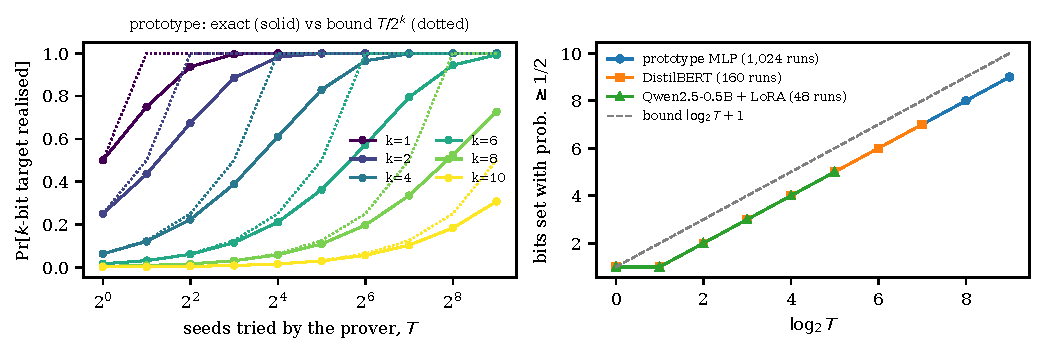
\includegraphics[width=0.8\textwidth]{fig/e3_grinding.pdf}
\caption{Seed grinding through a seed-accepting binding check. Left: prototype
(\EthreeN{} runs), exact probability of realising a random $k$-bit target (solid) and the
bound $T/2^k$ of Theorem~\ref{thm:grind} (dotted). Right: bits set with probability $\ge1/2$
for the prototype, DistilBERT (G1, \GOneN{} runs) and Qwen2.5-0.5B~+~LoRA (G4, \GFourN{}
runs); the three curves coincide where they overlap.}\label{fig:e3}
\end{figure*}

\subsection{Language-model scale (GPU)}

The prototype model is small. To check that binding by replay, grinding and detector
recall behave the same way for language models, we ran four experiments (G1--G4) on one consumer
GPU (NVIDIA \GPUname, 8\,GB; PyTorch \GPUtorch, CUDA \GPUcuda, Transformers \GPUtf) using
SST-2~\cite{socher2013sst}. The models were DistilBERT (\texttt{distilbert-base-uncased},
full fine-tuning) and Qwen2.5-0.5B with LoRA~\cite{hu2022lora} (rank 8 on the query and
value projections, sequence-classification head). Training ran in bf16 autocast, one
epoch, maximum length 64. A fifth experiment (G5) ran on a second machine, described below.

\paragraph{G2: exact replay}
Each configuration was trained three times from the same seed on 1,000 examples, both with
PyTorch's deterministic-algorithms mode and with default kernels (Table~\ref{tab:g2}). In
all four configurations the three runs produced bit-identical weights. Re-execution is
therefore a valid \textsf{BindFix}/\textsf{BindGrind} realisation for fine-tuning at this
scale on fixed hardware and software. Across machines it is not: G5 below re-executed nine
G3 runs on a second GPU with newer software, and none reproduced.

\begin{table}[t]
\centering\scriptsize
\caption{G2: replay of fine-tuning on one GPU (3 runs per row, same seed and data).}\label{tab:g2}
\resizebox{\columnwidth}{!}{\begin{tabular}{@{}llrcrr@{}}
\toprule
Model & kernels & trainable params & distinct hashes & max $|\Delta w|$ & train s\\
\midrule
\csname @@input\endcsname gen/tab_g2_rows.tex
\bottomrule
\end{tabular}}
\end{table}

\paragraph{G3: authorised-source poison at LLM scale}
An authorised source contributes $n$ dirty-label backdoor examples (negative sentences with
the trigger ``cf'' inserted, relabelled positive) to an 8,000-example committed set. Every
example carries a valid content-addressed Ed25519 receipt, so every provenance check
passes. We then measure the backdoor's attack success on triggered negative validation
sentences, and the recall of spectral signatures on DistilBERT's final-layer
\texttt{[CLS]} representation, flagging $1.5\varepsilon n_c$ items per class with
$\varepsilon=0.05$ (Table~\ref{tab:g3}).

\paragraph{Statistical treatment}
The replication unit is the training run (seed). Validation sentences within one run are not
independent replications of the model, so we report run-level values. For each run we give a
Wilson 95\% interval for its proportions, over $n=428$ triggered negative validation sentences
(attack success) and $n$ poisoned items (recall). We also give the attack success minus that of
the clean model with the same seed (\emph{baseline-adjusted}). With three seeds per condition
we report descriptive statistics only. A significance test over three runs would carry little
information (Table~\ref{tab:g3stats}).

The two curves cross. At 0.25--1\% poison, the detector finds 68--83\% of poisoned items on
average, but the backdoor has not taken hold after one epoch: mean baseline-adjusted attack
success stays between $-1$ and $+4$ points, with one run reaching $+9$ points at 1\%. At 2\%, the backdoor is effective in all three
runs, but unequally: baseline-adjusted attack success is $+\GthreeAdjHigh$ points on average,
ranging from $+\GthreeAdjHighMin$ to $+\GthreeAdjHighMax$. Mean recall falls to 25\%, with
wide per-run intervals.

Precision is the practical problem. The flag budget ($1.5\varepsilon n_c$ per class) sends
about \GthreeFPHigh{} clean examples per run to review at 2\% poison
(\GthreeFPRHigh\% of clean items). Only \GthreePrecHigh\% of flagged items are poisoned at 2\%,
and \GthreePrecLow\% at 0.25\%. A reviewer who inspects every flag therefore reads hundreds of
clean sentences per run, and still misses most of the poison where it matters. These are
results for one detector, one model and one trigger. They do not characterise poisoning
detection in general.

An auditor who holds a valid provenance record for this model holds no evidence about the
backdoor. This is Theorem~\ref{thm:content} measured on a pretrained transformer.
G5 below adds two detectors, a clean-data baseline and a higher poison level at GPU scale.

\begin{table}[t]
\centering\scriptsize
\caption{G3 summary: authorised-source backdoor poison, DistilBERT on SST-2 (3 seeds; mean
and range). Attack success over $n=428$ triggered negative sentences per run; clean accuracy
over $n=872$.}\label{tab:g3}
\resizebox{\columnwidth}{!}{\begin{tabular}{@{}rrclllr@{}}
\toprule
$n$ & rate & receipts & attack succ. & clean acc. & recall\phantom{x} & flagged\\
\midrule
\csname @@input\endcsname gen/tab_g3_rows.tex
\bottomrule
\end{tabular}}
\end{table}

\begin{table*}[t]
\centering\scriptsize
\caption{G3 per run (seeds 1, 2, 3). Attack success and recall in \% with Wilson 95\%
intervals; attack success over $n=428$ triggered negative sentences, recall over the $n$ poisoned
items. ``Adj.'': mean attack success minus the clean model's with the same seed, in percentage
points. FP: clean items flagged, mean over runs (rate over 8,000 clean items).}\label{tab:g3stats}
\begin{tabular}{@{}rp{6.2cm}rp{5.2cm}r@{}}
\toprule
$n$ & attack success per run [95\% CI] & adj. & recall per run [95\% CI] & FP (rate)\\
\midrule
\csname @@input\endcsname gen/tab_g3_stats_rows.tex
\bottomrule
\end{tabular}
\end{table*}

\paragraph{G5: three detectors and a second machine}
We added G5 in revision. It repeats the G3 protocol unchanged (same code, data, trigger,
seeds and training settings) at 0, 80, 160 and 320 poisoned items (0--3.8\%), and scores every
committed item with the three detectors of E2d, using the E2d flagging rules fixed before
the run. Unlike E2d, the detectors are applied to the trained model itself, as in G3. Because
the RTX~3070 machine was not available, G5 ran on a second machine: an NVIDIA \GFiveGPU{}
(\GFiveMem\,GB; PyTorch \GFiveTorch, CUDA \GFiveCuda, Python \GFivePy, Transformers \GFiveTf),
with deterministic kernels throughout, \GFiveTrainS\,s of training per run and at most
\GFivePeakGB\,GB of GPU memory. All \GFiveRuns{} runs completed, and \GFiveChecksOK{} of
\GFiveChecks{} automatic validity checks passed. The two that failed are the expected device
and the exact replay of G3, discussed next. Table~\ref{tab:g5} gives pooled recall and the
threshold-free AUROC within the target class, computed from the saved per-item scores.

\emph{Replay across machines.} Nine G5 runs (0, 80 and 160 poisoned items, seeds 1--3) are
exact re-executions of G3 runs. None reproduced G3's attack success, and \GFiveReplayAccEq{}
of \GFiveReplayN{} reproduced its clean accuracy. Below 2\% poison, attack success differed
by at most \GFiveReplayLowMaxDiff{} points; at 2\% it differed by up to \GFiveReplayMaxDiff{}
points for the same seed. GPU architecture and library versions changed together, so we
cannot attribute the difference to either. The practical consequence is clear: an auditor who
re-executes on a different stack does not obtain the trainer's model, so re-execution binding
needs a pinned hardware and software stack or a tolerance, and a tolerance enlarges
$\mathcal A_C$ (Theorem~\ref{thm:grind}).

\emph{Detection.} The qualitative results of G3 recur on the second machine. At 1\% poison
the backdoor has not taken hold, and the poison is easy to separate: AUROC
\GFiveSpecAucLow{} (spectral) and \GFiveLossAucLow{} (loss), with \GFiveSpecRecLow\% and
\GFiveLossRecLow\% recall within the flag budget, but only \GFiveSpecPrecLow\% precision. At
3.8\% the backdoor succeeds in every run (attack success at least \GFiveAsrHighMin\%), and
both detectors flag \GFiveRecHighTP{} of \GFiveHighN{} poisoned items; their AUROC
(\GFiveSpecAucHigh{} and \GFiveLossAucHigh) is at or below chance, so the poison looks
\emph{more} typical than clean data. Over the nine poisoned runs, recall falls as attack
success rises (Spearman $\rho=\GFiveRhoSpec$ for both; descriptive, since poison level drives
both; Fig.~\ref{fig:g5}). Activation clustering flagged a cluster in every run, including all three clean runs,
where it flagged \GFiveACCleanMin--\GFiveACCleanMax\% of clean items; its precision never
exceeded \GFiveACPrecMax\%. With this configuration it is not a usable detector here. These
results extend G3 to more detectors, a clean baseline and a higher poison rate; they use the
same model, data and trigger, so they say nothing about other models or attacks.

\begin{figure}[t]
\centering
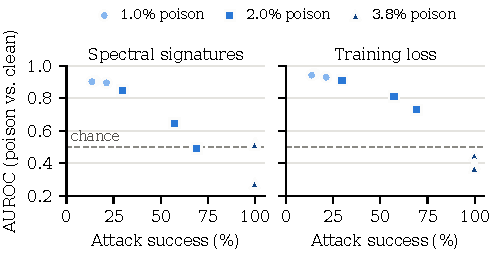
\includegraphics[width=\columnwidth]{fig/g5_detection.pdf}
\caption{G5: separability of poisoned from clean items (AUROC within the target class) against
the backdoor's attack success, one point per run. Detection is good only while the attack
fails; once the backdoor works in every run (3.8\% poison), both detectors are at or below
chance.}\label{fig:g5}
\end{figure}

\begin{table*}[t]
\centering\scriptsize
\caption{G5: three detectors on DistilBERT/SST-2 with authorised-source poison, run on a
second machine (\GFiveGPU; 3 seeds per row). Attack success: mean (range) over $n=428$
triggered negative sentences per run; clean accuracy over $n=872$. Recall: poisoned items
flagged out of all poisoned items over the 3 runs, flag budget $1.5\varepsilon n_c$ per class
($\varepsilon=0.05$, about 7.5\% of clean items by construction). AUROC: within the target
class, mean (range) over runs. Activation clustering: mean share of clean items flagged
(runs that flagged anything).}\label{tab:g5}
\begin{tabular}{@{}rrllllllr@{}}
\toprule
& & & & \multicolumn{2}{c}{spectral signatures} & \multicolumn{2}{c}{training loss} & act.\ clustering\\
$n$ & rate & attack succ.\ \% & clean acc.\ \% & recall & AUROC & recall & AUROC & clean FP\\
\midrule
\csname @@input\endcsname gen/tab_g5_rows.tex
\bottomrule
\end{tabular}
\end{table*}

\paragraph{G1 and G4: grinding at LLM scale}
We repeated E3 with \GOneN{} DistilBERT fine-tuning runs on a fixed 8,000-example committed set
(G1; \GOneTrainS\,s each; held-out accuracy $\GOneAcc\%\pm\GOneAccSd$; all \GOneDistinct{}
weight hashes distinct), and with \GFourN{} Qwen2.5-0.5B~+~LoRA runs on 2,000 examples
(G4; \GFourTrainS\,s each; accuracy $\GFourAcc\%\pm\GFourAccSd$). The probes, the disjoint
selection and evaluation seeds, and the exact analysis are the same as in E3. On the
selection seeds, \GOneSens\% (DistilBERT) and \GFourSens\% (Qwen~+~LoRA) of the 872 SST-2
validation sentences changed label across seeds.

The bits set with probability at least $1/2$ were exactly $\log_2T$ at every
$T\ge2$ for both models: \GOneBits{} bits at $T=\GOneTmax$ for DistilBERT and \GFourBits{}
bits at $T=\GFourTmax$ for Qwen~+~LoRA (Fig.~\ref{fig:e3}, right). This is the same curve as the
small prototype. In this setting, the channel's capacity is set by the number of training runs
the prover can afford, not by the model. Again the ground models were of ordinary quality:
\GOneChosenAcc\% against \GOneAllAcc\% for DistilBERT ($k=\GOneStK$, $T=\GOneStT$), and
\GFourChosenAcc\% against \GFourAllAcc\% for Qwen~+~LoRA ($k=\GFourStK$, $T=\GFourStT$).
At the measured training times, setting 7 chosen bits of a DistilBERT fine-tune takes under an hour
on a laptop GPU.

\subsection{Cost of record-level mechanisms (E4)}

\begin{table}[t]
\centering\scriptsize
\caption{Cost of record-level mechanisms on one CPU core (1\,KiB items). Per-item costs in
$\mu$s. Merkle root over all items in ms.}\label{tab:e4}
\setlength{\tabcolsep}{4.5pt}\begin{tabular}{@{}rrrrrrr@{}}
\toprule
items & hash & sign rcpt & verify rcpt & root (ms) & proof len & receipts (MB)\\
\midrule
\csname @@input\endcsname gen/tab_e4_rows.tex 
\bottomrule
\end{tabular}
\end{table}

Table~\ref{tab:e4} shows that hashing, receipts and commitments cost microseconds per item
and scale linearly. At the measured rate, verifying receipts for a corpus of $10^9$ documents would take about
\EfourVerifyHours{} core-hours, and the work is trivially parallel. The dominant cost of any
configuration that includes binding is binding itself. Exact re-execution doubles training,
and proof systems cost much more~\cite{abbaszadeh2024zkpot,liao2026verilora}.

\subsection{Published systems through the model (E1)}

Table~\ref{tab:e1} maps published systems to the model and reads off the goals they support.
The mapping uses each paper's own description of its mechanisms and trust assumptions. For
Atlas and VAMP we read the threat-model sections. For the others the mapping is from the
abstract and is marked as such.

\begin{table*}[t]
\centering\scriptsize
\caption{Published systems mapped to the model. ``Profile'' is the closest adversary profile
implied by the paper's threat model. Mechanisms marked $\tau$ are realised by trusted
hardware and are lost under \textsf{AdvTEE}.}\label{tab:e1}
\begin{tabular}{@{}p{2.3cm}p{3.6cm}p{2.1cm}p{4.6cm}p{3.6cm}@{}}
\toprule
System & Mechanisms (as described) & Profile & Goals supported per the model & Remark\\
\midrule
Atlas~\cite{spoczynski2025atlas} (threat model read) & TEE attestation of every transformation and its inputs; transparency log & MLaaS provider, hubs, producers untrusted $\approx$ full & With CPU-only TEEs and GPU training outside them (the paper's own limitation): $G_{\mathrm{compl}}$ only. With attested training (Bind under $\tau$): $G_{\mathrm{bind}}$, $G_{\mathrm{auth}}$ via AC+AT+$\beta$ & Dataset benignity out of scope, consistent with Thm.~\ref{thm:content}\\
Laminator~\cite{duddu2025laminator} (abstract) & Hardware-attested property cards for data, training, inference & full & Attested claims only under $\tau$; under full+tee none remain & No content claim beyond attested properties\\
VAMP~\cite{stokes2021prevent} (threat model read) & Signed manifests over datasets, software, models (WitSrc) & Infrastructure trusted $\approx$ trans-only & $G_{\mathrm{auth}}$ for filter-only pipelines; no $G_{\mathrm{zero}}$ & Title claims poisoning \emph{prevention}; holds for unauthorised modification only (Thm.~\ref{thm:content}.1)\\
PoL~\cite{jia2021pol} & Spot-check re-execution with tolerance, prover-chosen randomness & exec-only & $G_{\mathrm{bind}}$ up to spoofing~\cite{fang2023pol}; not $G_{\mathrm{noinf}}$ (BindGrind) & Tolerance enlarges the grinding set (Thm.~\ref{thm:grind})\\
VeriLoRA~\cite{liao2026verilora} (protocol sections read) & ZK proof of every LoRA step (forward, backward, update); initial weights committed as part of the witness & exec-only & $G_{\mathrm{bind}}$ as \textsf{BindGrind}: the paper does not fix mini-batch sampling or initialisation randomness by the verifier, so not $G_{\mathrm{noinf}}$; no dataset commitment is described, so binding to a record needs one; no lineage without WitSrc or attestation & Combine with a beacon-derived seed and data commitment to obtain \textsf{BindFix}\\
Kaizen zkPoT~\cite{abbaszadeh2024zkpot} (protocol sections read) & ZK proof of every training iteration over a Merkle-committed dataset; prover commits the initial weights; batch order from a public pseudorandom permutation key & exec-only & $G_{\mathrm{bind}}$ as \textsf{BindGrind}: the prover commits its own initial weights, the protocol does not require the permutation key to be fixed by the verifier after the data commitment, and the number of proved iterations need not be fixed in advance, so not $G_{\mathrm{noinf}}$; no lineage without WitSrc or attestation & Seed rejection sampling against zkPoTs demonstrated by~\cite{tan2025zkpot}\\
Optimum-vicinity zkPoT~\cite{tan2025zkpot} (full text read) & ZK proof that the released model is within $\epsilon$ of the optimum of an $L_2$-regularised convex loss on the committed data & exec-only & $G_{\mathrm{bind}}$ with $\mathcal A_C$ an $\epsilon$-ball, independent of training randomness; influence bounded geometrically rather than by $T$ & Logistic regression and SVMs; no lineage or content claim\\
AuditableLLM~\cite{li2025auditablellm} (abstract) & Hash-chained audit trail of updates & exec-only & Store integrity ($P_1$) only; no pipeline goal & ``Verifiable integrity'' is of the log, not of the training\\
Mehammed et al.~\cite{mehammed2025fl} (abstract) & Permissioned ledger, update audit, zk-SNARK of client summaries & full (clients untrusted) & $P_1,P_2,P_8$; no binding of client training, so no pipeline goal & Ledger contributes $P_8$ (Prop.~\ref{prop:ledger})\\
\bottomrule
\end{tabular}
\end{table*}

The pattern is consistent. Systems that state a narrow threat model (Atlas and VAMP, which
trust the verification or training infrastructure) make claims that the model supports
within that model. The model's value is that it says what changes when the trust assumption
does not hold. Claims phrased as preventing poisoning, or as verifiable integrity of
training, hold only for the narrower properties the model identifies.

% ---------------------------------------------------------------
\section{Literature Search Method}\label{sec:lit}
% ---------------------------------------------------------------

The systematisation in Section~\ref{sec:sok} rests on a structured search. We report it
in PRISMA~2020 terms~\cite{page2021prisma} and state plainly which stages are incomplete.

\paragraph{Search}
On 25~October~2026 we ran 12 query strings against OpenAlex. The strings cover provenance
and lineage capture, ledgers, transparency logs, trusted execution, proofs of learning,
zero-knowledge training proofs, data-use auditing and poisoning defences. We retrieved
the first 25--100 results per string (24 result pages in total, depth by string as
recorded in the artefact). This produced 594 records. A version-aware deduplication kept
the peer-reviewed version of each work and recorded all its DOIs, which removed 43
duplicates.

\paragraph{Eligibility}
Inclusion required (I1) an ML or AI training pipeline, (I2) a mechanism for provenance,
integrity or verification of training data or training computation, and (I3) peer review.
Exclusion codes covered: no ML context (E1); inference-output provenance only (E2);
document types outside the protocol (E3); poisoning work without a provenance or
verification component (E5); and preprint-only works (E7). E7 works were kept in a
separate positioning list and are not cited as evidence.

\paragraph{Screening}
A rule-based pre-screen excluded 248 of 551 records: 135 preprint-only, 90 without ML or
provenance terms, and 23 by document type. An audit of 92 rule exclusions by title found
2 false exclusions, which were restored. Title-and-abstract screening of the remaining 303
records was carried out by an AI assistant (Claude) applying the written protocol. Every
decision is logged with a reason code and labelled as an AI decision requiring human
verification. It excluded 154 records and passed 149 (55 marked \emph{unsure}). Nine further
records came from citation chasing. That leaves 158 records for full-text assessment.

\paragraph{Status and limits}
\pending{Full-text screening of the 158 records, a human second screener with reported
agreement ($\kappa$) on at least a 20\% sample, and searches of Scopus, Web of Science,
IEEE~Xplore and the ACM Digital Library are not yet complete. Until they are, the search
is a structured mapping, not a systematic review.} A known-item check found 8 of 17 seed
papers that the authors had identified beforehand. The misses include Atlas and Sigstore,
which is why the database searches above are required before submission. The screening log,
queries and raw result pages are part of the artefact.

% ---------------------------------------------------------------
\section{Discussion}\label{sec:discussion}
% ---------------------------------------------------------------

\subsection{What an auditor may conclude}

\begin{figure}[t]
\centering
\resizebox{\columnwidth}{!}{% Fig.: what an auditor may conclude (Discussion), column width
\begin{tikzpicture}[font=\sffamily\scriptsize, >={Stealth[length=1.6mm]},
  q/.style={draw=black!55, fill=black!4, rounded corners=2pt, text width=24mm, align=center,
            inner sep=2pt, minimum height=13mm,
            execute at begin node={\hyphenpenalty=10000\exhyphenpenalty=10000}},
  a/.style={draw=black!30, fill=white, rounded corners=2pt, text width=47mm, align=flush left,
            inner sep=2.5pt, minimum height=13mm,
            execute at begin node={\hyphenpenalty=10000\exhyphenpenalty=10000}},
  fl/.style={->, black!65, line width=0.6pt}]
\newcommand{\Y}{\textcolor{okgreen}{\textbf{yes}}}
\newcommand{\N}{\textcolor{advorange}{\textbf{no}}}
\def\dy{1.65}
\node[q] (q1) at (0,0)      {\textbf{1} Is the trainer trusted?};
\node[q] (q2) at (0,-\dy)   {\textbf{2} Does the verifier fix the seed after the data commitment?};
\node[q] (q3) at (0,-2*\dy) {\textbf{3} Is there an authenticated route from sources to training?};
\node[q] (q4) at (0,-3*\dy) {\textbf{4} Is the model free of poison?};
\node[a, right=3mm of q1] (a1) {\Y: attested capture binds the model to its record; no proof of training needed.\\
  \N: binding (exact replay or a proof of training) is required. \hfill\textcolor{black!55}{Thm.~\ref{thm:bind}}};
\node[a, right=3mm of q2] (a2) {\Y: no prover influence, if replay is exact on a pinned stack.\\
  \N: up to $\log_2 T$ chosen bits for $T$ runs. \hfill\textcolor{black!55}{Thms.~\ref{thm:noinf},~\ref{thm:grind}; G2, G5}};
\node[a, right=3mm of q3] (a3) {\Y, with binding: lineage holds via source witnesses or attested capture and transform; stage types must be declared. \N: no lineage claim. \hfill\textcolor{black!55}{Thm.~\ref{thm:auth}, Cor.~\ref{cor:launder}}};
\node[a, right=3mm of q4, draw=advorange, fill=advorange!7] (a4) {Never certified. At best: every poisoned item used was missed by the detector, worth its recall, which collapsed once the backdoor worked. \hfill\textcolor{black!55}{Thm.~\ref{thm:content}; G3, G5}};
\foreach \i [count=\j from 2] in {1,2,3} \draw[fl] (q\i) -- (q\j);
\foreach \i in {1,...,4} \draw[fl] (q\i) -- (a\i);
\end{tikzpicture}
}
\caption{Four questions an auditor should answer before accepting a claim about a released
model, and what the theorems and experiments say for each answer.}
\label{fig:auditor}
\end{figure}

Table~\ref{tab:minimal} can be read as a checklist, and Fig.~\ref{fig:auditor} condenses it
into four questions. Before accepting a claim about a
released model, an auditor should establish three things:
\begin{enumerate}
\item Who is trusted: which profile applies.
\item Which mechanisms were actually deployed and verified.
\item Which goal the claim corresponds to.
\end{enumerate}
Two examples show how this works.

A cloud provider's attested data pipeline without binding (\textsf{AttCap}, \textsf{AttTrans}
under the full adversary) supports no claim about the released model. It does support the
record-level claim $G_{\mathrm{compl}}$.

A signed-manifest scheme with a trusted training infrastructure (the trans-only or cap-only
profiles) does support lineage for filter-only pipelines, but not the absence of poison.

\subsection{Answers to five design questions}

\paragraph{Binding}
Binding is required whenever the trainer is not trusted, and no amount of witnessing or
attestation of earlier stages substitutes for it (Theorem~\ref{thm:bind}). If binding is
used, its randomness must be fixed after commitment (Theorems~\ref{thm:noinf}
and~\ref{thm:grind}). Exact re-execution is a valid binding only where training is
bit-reproducible. Section~\ref{sec:eval} measures when it is.

\paragraph{Witnessing}
Source receipts must be content-addressed (split view, Section~\ref{sec:eval}). Source
witnessing and input witnessing answer different questions, lineage and completeness. Each
fails under collusion, so witnesses should be organisationally independent of the operator
they observe.

\paragraph{Synthetic data}
Generative stages need an attested transform even on the witness route, and stage types
must be declared and authenticated (Corollary~\ref{cor:launder}). Lineage of synthetic data
is recursive: the generator is itself a model whose provenance matters. Our model treats it
as an authorised but possibly poisoned source (\textsf{AdvGen}).

\paragraph{Blockchain versus transparency logs}
For every goal we study, a witnessed transparency log is sufficient as the record store.
A ledger adds inclusion liveness (Proposition~\ref{prop:ledger}). We find no support for
the claim that a blockchain makes training records complete or truthful. Those properties
are decided upstream of the store.

\paragraph{Poisoning}
Provenance cannot certify that a model is poison-free (Theorem~\ref{thm:content}). It can
make a detector's verdict \emph{transfer} to the released model, which is what binding and
completeness contribute. The resulting claim is only as strong as the detector's recall.
In our experiments, recall was weakest exactly where the poison worked. The prototype's detector flagged at most a quarter of the planted items. On DistilBERT, recall fell from 68--83\% at the lower, ineffective poison rates to 25\% at the 2\% rate where the backdoor took hold (Section~\ref{sec:eval}). Any
certification scheme that reports provenance without detector recall overstates its
assurance.

\subsection{Open problems}

\begin{enumerate}
\item \emph{Binding at pre-training scale.} Zero-knowledge binding now reaches LoRA
  fine-tuning~\cite{liao2026verilora}, but not full pre-training. Exact re-execution
  doubles the cost and requires determinism. Spot-check proofs of learning admit spoofing
  under tolerance~\cite{fang2023pol}.
\item \emph{Tolerance as a grinding channel.} Theorem~\ref{thm:grind} bounds influence by the
  number of accepted trajectories. For tolerance-based verifiers that number is not
  characterised. Optimum vicinity~\cite{tan2025zkpot} closes the channel for convex
  objectives; for non-convex LLM training it remains open.
\item \emph{Attested accelerators.} The attestation routes assume that the relevant stages run
  in TEEs. Atlas notes that GPUs lack equivalent protection~\cite{spoczynski2025atlas}.
\item \emph{Detector guarantees.} $G_{\mathrm{content}}$ is parameterised by recall. Certified
  recall bounds for poisoning detectors at LLM scale are lacking.
\item \emph{Confidential verifiability ($P_7$).} All our mechanisms reveal the record to the
  auditor. Combining them with confidentiality of training data is open.
\item \emph{Composition across model generations.} Fine-tuning chains and synthetic data make
  provenance recursive. The model covers one training run.
\end{enumerate}

\subsection{Limitations}

\paragraph{Model}
The model has five abstractions:
\begin{itemize}
\item Items are atomic and content-identified.
\item Each mechanism is all-or-nothing.
\item A single training run is modelled.
\item Detectors are abstracted to an examined set and a miss set, with no budget or base
  rate.
\item Correlated compromise is captured \emph{across} trust anchors (any subset of
  capabilities), but not \emph{within} a mechanism class, such as one corrupt witness among
  several.
\end{itemize}
Table~\ref{tab:scope} lists which training practices fall inside the abstraction. The
model's results are exact for the model only. Their relevance to real systems rests on the
validation in Section~\ref{sec:eval}.

\paragraph{Prototype}
The prototype trains a small bag-of-words network on 2,000 reviews. It simulates trusted
execution with key isolation rather than real enclaves, so it validates the logic of
attestation-based checks, not any hardware. It compares three detectors on one small model. Poisoning at GPU scale was
measured on one model (DistilBERT), one dirty-label trigger and three seeds per condition,
with one detector in G3 and three in G5, so it is reported descriptively. G5 ran on a second,
smaller GPU because the first was unavailable; its qualitative results match G3, but its runs
did not replay G3's bit for bit. Bit-exact replay therefore holds on a fixed stack only, and
we changed GPU and library versions together, so we cannot say which change breaks it. The
GPU experiments cover fine-tuning, not pre-training.
Their seed counts (160 and 48) limit the largest $T$ we could test to 128 and 32.

\paragraph{Literature}
The literature search used one database, title-and-abstract screening was performed by an
AI assistant, and full-text assessment is pending (Section~\ref{sec:lit}). The case-study
mapping relies partly on abstracts.

\paragraph{Proofs}
The proofs are by hand. They are backed by two independent exhaustive decision procedures
for the six profiles, and by a third, vectorised checker over all 128 adversary subsets. They
are not mechanised in a proof assistant. Proposition~\ref{prop:ledger} and the composition
remark of Section~\ref{sec:scope} are argued, not proved.


\section{Artefact, Data, Ethics and AI-Use Statement}\label{sec:artefact}
\paragraph{Artefact}
The artefact contains:
\begin{itemize}
\item the Alloy models, the sweep, the independent checker, the adversary-lattice checker and
  their raw outputs;
\item the prototype and every experiment script with raw and processed results;
\item the GPU kit with its logs;
\item the G5 kit, its logs and per-item detector scores;
\item the literature-search queries, raw result pages and screening log;
\item SHA-256 manifests and a reproducibility guide that regenerates every table and figure.
\end{itemize}
The artefact is archived on Zenodo, version~1.1:
\url{https://doi.org/10.5281/zenodo.24420107} (all versions:
\url{https://doi.org/10.5281/zenodo.24317966}). Code is released under the MIT licence and
results, data and documentation under CC~BY~4.0. A working copy is maintained at
\url{https://github.com/waqas6755/what-can-provenance-prove}. The archive holds a reproducibility
guide that maps each table and figure to the script and raw file that produce it, and SHA-256
checksums of its files.

\paragraph{Data, models and licences}
The prototype uses the polarity dataset v2.0~\cite{pang2004sentimental}, as distributed by
NLTK. The GPU experiments use SST-2~\cite{socher2013sst} from the GLUE distribution, with
\texttt{distilbert-base-uncased} and \texttt{Qwen/Qwen2.5-0.5B} from the Hugging Face Hub. No
personal data is processed. Both models are released under the Apache~2.0 licence. Neither the
polarity dataset nor the Stanford Sentiment Treebank states a licence: the polarity dataset's
distribution page asks users to cite its version number, and the GLUE distribution refers users to
the licence of each source dataset. We use both datasets unmodified, for research only, and do not
redistribute them; the artefact gives download instructions instead.

\paragraph{Dual use and disclosure}
The attacks we implement (split-view delivery, laundering, seed grinding, authorised-source
backdoors) are either already published or follow directly from the model. They are run only
against our own prototype and public models. The grinding result points to a simple
mitigation, a beacon-fixed seed, which we recommend to builders of proof-of-training systems.
No third-party system was attacked.

\paragraph{AI assistance}
An AI assistant (Claude, Anthropic) was used to:
\begin{itemize}
\item write experiment and analysis code;
\item run the model checker and the experiments in the cloud environment;
\item draft and revise text;
\item perform title-and-abstract screening.
\end{itemize}
The AI screening decisions are labelled as such in the released log. They have not been
verified by a human screener, and they are not reported as independent human screening. The
authors are responsible for verifying the code, results and proofs, and for all claims.
\pending{State which verification the authors have personally carried out.} \pending{Check this statement against the journal's current AI-use policy before
submission.}

\section{Conclusion}
We separate the conclusions by the kind of evidence behind them.

\paragraph{Proved within the model}
\begin{itemize}
\item Computation binding is necessary exactly when the trainer is untrusted.
\item Lineage has two routes with disjoint trust anchors.
\item Generative pipelines need authenticated stage types.
\item A seed-accepting binding check leaks at most $\log_2T$ bits for $T$ evaluated accepted
  outputs.
\item No mechanism set certifies the absence of poison; the strongest claim is conditional on
  a detector.
\item Attested capture and input witnessing are interchangeable for record completeness.
\end{itemize}
These statements hold for every subset of adversary capabilities. They are exact for the
abstract single-run model of Section~\ref{sec:model}, within the scope of
Table~\ref{tab:scope}.

\paragraph{Observed in our experiments}
\begin{itemize}
\item A prototype with real cryptography and simulated trusted execution matched the model
  on all 9,216 instances.
\item Seed grinding reached $\log_2T$ bits on a small model, on DistilBERT and on Qwen
  2.5-0.5B~+~LoRA.
\item Fine-tuning replayed bit for bit on one machine, but not on a second machine with a
  different GPU and newer libraries.
\item One spectral-signature detector lost most of its recall exactly where an
  authorised-source backdoor became effective, at low precision.
\item On the prototype, three detectors, including a loss score and activation clustering,
  showed the same pattern or found nothing.
\item At GPU scale, spectral and loss detectors separated poison well at 1\% poison and fell
  to chance at 3.8\%, where the backdoor always worked; activation clustering flagged about a
  quarter of clean data even with no poison.
\end{itemize}

\paragraph{From the literature}
The surveyed systems make claims that hold within their own trust assumptions. Claims of
poisoning prevention, or of verifiable integrity of training, hold only for the narrower
properties identified in Table~\ref{tab:e1}. This conclusion rests on a structured mapping,
not yet a systematic review (Section~\ref{sec:lit}).

\paragraph{Design rules and future work}
\begin{itemize}
\item Bind the computation whenever the trainer is untrusted, with randomness fixed after
  commitment.
\item Use content-addressed receipts and authenticated stage types.
\item Diversify trust anchors.
\item Report detector recall and precision alongside any content claim.
\item Use a ledger only where censorship-resistant inclusion is itself a requirement.
\end{itemize}
Future work includes binding at pre-training scale, replay across hardware stacks (which
failed in our one cross-machine test), multi-stage and
multi-parent model lineages, real enclave deployments, and detectors with guaranteed recall.

\bibliographystyle{IEEEtran}
\bibliography{refs}

\ifproofsinpaper
\appendices
% ---------------------------------------------------------------
\section{Proofs}\label{app:proofs}
% ---------------------------------------------------------------

Throughout, an execution is written $E=(\mathcal I,\{v_i\}_{i\in\mathcal I},g)$. Here
$v_i\in\{0,1\}^{11}$ records the membership of item $i$ in
$D,S,F,C,U,\hat S,\hat D,\hat F,B,M,X$, and $g$ collects the global Booleans: $\alpha$,
$\mu$, $\mathit{gen}$, $\mathit{gs}$, and whether the detector is perfect. We write
$i\in D$ for $v_i[D]=1$. A \emph{counterexample} to $\mu\models_{\alpha,\mathit{gen}}G$ is an
admissible, accepted execution that violates $G$. In every construction below, $X$ is set
equal to $C$ whenever $\textsf{Detector}\in\mu$ and $\tau$ hold, as $\Phi_8$ requires, and
the listed items are not in $B$ unless stated. We leave $X$ out of the listed vectors.

\subsection*{Proof of Lemma~\ref{lem:sep} (Separability)}

\emph{Form of the constraints.}
Each set equation or inclusion between sets in $\Phi$, $\mathrm A$ and the goals is a
universally quantified per-item statement. For example, $C\subseteq\hat D\cup\hat S$ is
$\forall i.\ i\in C\Rightarrow(i\in\hat D\vee i\in\hat S)$, and $U=C$ is
$\forall i.\ i\in U\Leftrightarrow i\in C$. Emptiness ($S=\emptyset$) and disjointness
($D\cap S=\emptyset$) are also per-item. Each premise of an implication in $\Phi$ or
$\mathrm A$ (``$\textsf{AdvTrans}\notin\alpha$'', ``$\beta$'', ``$\mathit{gen}$'') mentions
only global Booleans. Hence each constraint has the form
$\psi(g)\Rightarrow\forall i.\ \varphi(v_i,g)$, which equals
$\forall i.\ (\psi(g)\Rightarrow\varphi(v_i,g))$ whenever $\mathcal I\neq\emptyset$.
Two constraints mention only $g$:
$\mathit{gs}\Rightarrow(\textsf{AdvExec}\in\alpha\wedge\textsf{BindFix}\notin\mu)$ in
$\Phi_6$, and the conjunct $\neg\mathit{gs}$ of $G_{\mathrm{noinf}}$. Write the admissible,
accepted executions as those satisfying
$\chi_\Phi(g)\wedge\forall i.\ \varphi_\Phi(v_i,g)$, and each goal as
$\chi_G(g)\wedge\forall i.\ \varphi_G(v_i,g)$.

\emph{The zero vector.}
Let $\mathbf 0$ be the vector with every membership $0$. Every per-item constraint holds
at $\mathbf 0$. Every inclusion $P\subseteq Q$ holds because $i\notin P$. Every equation
$P=Q$ holds because both sides are false. Every emptiness and disjointness condition holds
trivially. Each $\varphi_G$ holds at $\mathbf 0$ for the same reasons. (This side condition
is also asserted mechanically by our independent checker.)

\emph{Reduction.}
($\Leftarrow$) Let $E$ be a counterexample over $\mathcal I$. Then $\chi_\Phi(g)$ holds,
$\varphi_\Phi(v_i,g)$ holds for every $i$, and either $\chi_G(g)$ fails or
$\varphi_G(v_{i_0},g)$ fails for some $i_0$. In the first case, the one-item execution
$(\{j\},v_j{=}\mathbf 0,g)$ is admissible, accepted and violates $\chi_G$. In the second,
the restriction $(\{i_0\},v_{i_0},g)$ is admissible and accepted (its only item satisfied
every per-item constraint in $E$), and it violates $\varphi_G$. Either way there is a
one-item counterexample.
($\Rightarrow$) Given a one-item counterexample $(\{i_0\},v_{i_0},g)$ and any universe
$\mathcal I\ni i_0$, assign $\mathbf 0$ to every other item. The new items satisfy every
per-item constraint and goal, so the extended execution is admissible, accepted and still
violating. Hence a counterexample exists over some universe iff one exists over a single
item. \qed

\emph{The empty universe.} If $\mathcal I=\emptyset$, only the global conditions $\chi$
remain. Any counterexample there violates some $\chi_G$. It is then reproduced by the
one-item execution with the zero vector, which is admissible and accepted. So restricting
the check to one item loses nothing.

\emph{When the lemma fails.} The lemma uses two facts: every constraint is a per-item
universal statement or a global condition, and the zero vector satisfies every per-item
constraint. A constraint that relates different items breaks the first fact. Examples are a
cardinality bound (``at most $n$ items are flagged'', a detector \emph{budget}), a ratio (``at
most $\varepsilon$ of $C$ is poisoned''), or a relation between runs (``$C_j$ contains
$M_{j-1}$''). Extensions with such constraints need bounded model checking, or a new argument.
This is why detector budgets and poison rates appear in our experiments and not in the
model.

\subsection*{Proof of Proposition~\ref{prop:mono} (Monotonicity)}

Let $\mu\subseteq\mu'$, and let $E'$ be a counterexample for $\mu'$. We build a
counterexample for $\mu$. Adding a mechanism has three effects. It adds acceptance
conditions ($\mathrm A_1$--$\mathrm A_4$). It strengthens admissibility constraints
($\Phi_3$--$\Phi_5$ only gain premises that make them apply). And it can enlarge $X$ from
$\emptyset$ to $C$ ($\Phi_8$). Take $E$ equal to $E'$ except that $X$ is recomputed by
$\Phi_8$ for $\mu$, and $\mathit{gs}$ is unchanged. Every constraint that applies under
$\mu$ also applies under $\mu'$, so $E$ is admissible and accepted. The one exception is
$\Phi_6$'s $\mathit{gs}$ clause, which is weaker under $\mu$ because $\mu$ has no more
\textsf{BindFix} than $\mu'$. $X$ occurs in the goals only on the right of an inclusion
($G_{\mathrm{content}}$), and $X_E\subseteq X_{E'}$. So any goal violated by $E'$ is
violated by $E$. \qed

\subsection*{Proof of Theorem~\ref{thm:bind} (Binding)}

\emph{Sufficiency.} $\beta$ with $(\mathrm A_1)$ gives $U=C$. If
$\textsf{AdvExec}\notin\alpha$, then $U=F$ by $\Phi_6$. Then $\textsf{AdvCap}\notin\alpha$
or $(\textsf{AttCap}\in\mu\wedge\tau)$ gives $C=F=U$ by $\Phi_5$.

\emph{Necessity.} Let $\textsf{AdvExec}\in\alpha$ and $\neg\beta$. Take one item with
$v=\{U\}$ (only $U$ set). No constraint of $\Phi$ mentions $U$ except $\Phi_6$, whose
premise fails. $(\mathrm A_1)$ is vacuous; $(\mathrm A_2)$ and $(\mathrm A_4)$ concern
$C=\emptyset$; $(\mathrm A_3)$ holds because $\hat F=F=\emptyset$. So the execution is
accepted, and $U\neq C$. Now let $\textsf{AdvExec}\notin\alpha$, $\textsf{AdvCap}\in\alpha$,
$\neg\beta$, and $\textsf{AttCap}\notin\mu$ or $\neg\tau$. Take $v=\{D,\hat D,C\}$. The item
is delivered and witnessed, but filtered out by an honest transform and re-added by a
corrupt capture. $F=U=\emptyset$, $C=\{i\}$; $(\mathrm A_2)$ holds because $i\in\hat D$, and
$(\mathrm A_3)$ holds because $\hat F=\emptyset$. Hence $U\neq C$. \qed

\subsection*{Proof of Theorem~\ref{thm:auth} (Lineage)}

Fix the full adversary, so $\tau$ holds, $\textsf{AdvWit}\notin\alpha$ and
$\hat D=D,\hat F=F$.

\emph{Sufficiency.} By $(\mathrm A_1)$, $U=C$.
(a) $\textsf{WitSrc}$, $\neg\mathit{gen}$: $(\mathrm A_2)$ gives $C\subseteq D\cup\hat S$,
and $\hat S=\emptyset$ by $\Phi_1$. Hence $U\subseteq D$.
(b) $\textsf{WitSrc}\wedge\textsf{AttTrans}$: $\hat S=S$ by $\Phi_4$, so
$U=C\subseteq D\cup S$.
(c) $\textsf{AttCap}\wedge\textsf{AttTrans}$: $C=F$ by $\Phi_5$ and $F\subseteq D\cup S$ by
$\Phi_3$, so $U\subseteq D\cup S$.

\emph{Necessity.} By monotonicity it suffices to refute the maximal mechanism sets outside
the stated condition. Each counterexample below has one item $x$ with $x\notin D\cup S$.
\begin{itemize}
\item $\neg\beta$ (all other mechanisms present): $v=\{U\}$, as in Theorem~\ref{thm:bind}.
\item $\beta$, no \textsf{WitSrc}, no \textsf{AttTrans}: $v=\{F,C,U,\hat F\}$. $\Phi_3$ does not
  apply ($\textsf{AdvTrans}$, no attestation), so $F$ is unconstrained.
  \textsf{AttCap} gives $C=F$, and $(\mathrm A_3)$ holds because $\hat F=F\subseteq C$.
\item $\beta$, no \textsf{WitSrc}, no \textsf{AttCap}: $v=\{C,U\}$. $\Phi_5$ does not apply,
  so $C$ is unconstrained. $F=\emptyset$ satisfies $\Phi_3$, and $(\mathrm A_3)$ is vacuous.
\item $\mathit{gen}$, $\beta$, \textsf{WitSrc}, no \textsf{AttTrans} (\textsf{AttCap},
  \textsf{WitIn}, \textsf{Detector} present): $v=\{F,C,U,\hat F,\hat S\}$. $\Phi_4$ does not
  apply, so $\hat S$ is unconstrained (the transform \emph{launders} $x$ as synthetic).
  $(\mathrm A_2)$ holds because $x\in\hat S$.
\end{itemize}
In every case $x\notin B$, so $(\mathrm A_4)$ holds, and $U\not\subseteq D\cup S$.

\emph{Colluding witnesses (full+wit).} $\Phi_7$ no longer applies, so $\hat D$ and
$\hat F$ are unconstrained. Every mechanism set without both \textsf{AttCap} and
\textsf{AttTrans} then fails. Without \textsf{AttTrans}, use $v=\{F,C,U,\hat D\}$.
Without \textsf{AttCap}, use $v=\{C,U,\hat D\}$. Proof (c) does not use witnesses, so the
attestation route still holds.

\emph{Broken attestation (full+tee).} $\tau$ fails, so $\Phi_3$--$\Phi_5$ never apply
through attestation, and $\hat S$ is unconstrained whenever $\mathit{gen}$ holds. For
filter-only pipelines, (a) still applies. For generative ones, the laundering instance
refutes every mechanism set. \qed

\subsection*{Proof of Corollary~\ref{cor:launder}}

Drop $\neg\mathit{gen}\Rightarrow\hat S=\emptyset$. Then the laundering instance of the last
bullet above is admissible for filter-only pipelines too. So
$\{\textsf{BindFix},\textsf{BindGrind},\textsf{WitSrc},\textsf{WitIn},\textsf{AttCap},\textsf{Detector}\}$
fails $G_{\mathrm{auth}}$. \qed

\subsection*{Proof of Theorem~\ref{thm:noinf} (Influence)}

If $\textsf{BindFix}\in\mu$, then $\Phi_6$ forces $\neg\mathit{gs}$, and $\beta$ gives
$U=C$. If $\textsf{BindFix}\notin\mu$, the execution with every item $\mathbf 0$ and
$\mathit{gs}$ true is admissible ($\textsf{AdvExec}\in\alpha$) and accepted, and it
violates $G_{\mathrm{noinf}}$. \qed

\subsection*{Proof of Theorem~\ref{thm:grind} (Grinding bound)}

Write the candidates as $\Sigma=\{M_1,\dots,M_T\}\subseteq\mathcal A_C$. By assumption
they are generated independently of $K$, so $(C,\Sigma)$ is independent of $K$. Given
$(C,\Sigma)$, the released $M$ is a function of the index $j^\ast$ with $M=M_{j^\ast}$.
Hence $H(M\mid C,\Sigma)\le H(j^\ast)\le\log_2T$. Since $I(K;M\mid C,\Sigma)\le
H(M\mid C,\Sigma)$, this gives $I(K;M\mid C,\Sigma)\le\log_2T$.

For the second claim, let $\pi(M)\in\{0,1\}^k$ be the behaviour pattern the adversary
targets. Given $(C,\Sigma)$, $\pi(M)$ takes values in the set
$P_{C,\Sigma}=\{\pi(M_j)\}_j$, which has at most $T$ elements. For $K$ uniform and
independent of $(C,\Sigma)$,
\[
\Pr[\pi(M)=K]\le\Pr[K\in P_{C,\Sigma}]=\mathbb E\,|P_{C,\Sigma}|/2^k\le T/2^k.
\]
The same bound holds if the prover evaluates the candidates one at a time and stops at the
first match. The patterns it can reach are still those of at most $T$ candidates drawn
independently of $K$. Success probability at least $1/2$ therefore requires $T\ge2^{k-1}$.

Under \textsf{BindFix}, the verifier recomputes the seed from the committed record and a
beacon released after commitment, and replays exactly. Then
$\mathcal A_C=\{\mathrm{Train}(C,s_{\mathrm{fix}})\}$, so $T=1$.

\emph{Scope of the proof.} The bound depends only on $|\Sigma|$. It does not assume that
candidates are distinct seeds, that training is deterministic, or that $\mathcal A_C$ is
small. Nondeterminism and tolerance enter only through the size of $\mathcal A_C$, and so
through how large a $T$ the prover can obtain. \qed

\subsection*{Proof of Theorem~\ref{thm:content} (Content)}

\emph{Part 1.} For any $\mu$, take one item with $v=\{D,\hat D,F,C,U,B,M\}$ and, if
\textsf{Detector} is present and $\tau$ holds, also $X$. This is a poisoned item from an
authorised source, missed by the detector. Admissibility: $B\cap D\neq\emptyset$ is
allowed by \textsf{AdvSource}; $F\subseteq D$, $C=F$, $U=F$; $\hat S=S=\emptyset$. Acceptance:
$U=C$; $C\subseteq\hat D$; $\hat F\subseteq C$; $C\cap B\subseteq M$. The execution violates
$G_{\mathrm{zero}}$. With a perfect detector $M=\emptyset$, $(\mathrm A_4)$ gives
$C\cap B=\emptyset$, and $\beta$ gives $U\cap B=C\cap B=\emptyset$.

\emph{Part 2.} Sufficiency: $\beta$ gives $U=C$. \textsf{Detector} with $\tau$ gives $X=C$
and $C\cap B\subseteq M$. Hence $U\cap B=C\cap B\subseteq M\cap C=M\cap X$. Necessity:
without $\beta$, take $v=\{D,\hat D,U,B\}$. The item is poisoned and delivered; the transform
dropped it, the record does not contain it, and the corrupt executor trains on it anyway.
$C=\emptyset$, so $X=\emptyset$.
Without \textsf{Detector}, take the Part~1 item without $X$; then $X=\emptyset$, so
$U\cap B\not\subseteq X$.

\emph{Part 3.} With $\textsf{AdvExec}\notin\alpha$, $U=F$. Sufficiency: if
$\mu\models G_{\mathrm{compl}}$, then $F\subseteq C$. With \textsf{Detector} and $\tau$,
$U\cap B=F\cap B\subseteq C\cap B\subseteq M$, and $\subseteq C=X$. Necessity: without
\textsf{Detector}, $X=\emptyset$ and the Part~1 item refutes. If
$\mu\not\models G_{\mathrm{compl}}$, take a one-item counterexample to $G_{\mathrm{compl}}$
($i\in F$, $i\notin C$). By Theorem~\ref{thm:compl}'s necessity construction it can be
chosen with $i\in D\cap\hat D$, and setting $i\in B$ affects no constraint. Since
$i\notin C=X$, $U\cap B\not\subseteq X$.

\emph{Broken attestation.} If $\tau$ fails, $X=\emptyset$ by $\Phi_8$, and the Part~1 item
violates $G_{\mathrm{content}}$ for every $\mu$. \qed

\subsection*{Proof of Theorem~\ref{thm:compl} (Completeness)}

\emph{Sufficiency.} $\textsf{AttCap}\wedge\tau$: $C=F$. $\textsf{WitIn}$ with
$\textsf{AdvWit}\notin\alpha$: $\hat F=F$ and $(\mathrm A_3)$ give $F\subseteq C$.
$\beta$ with $\textsf{AdvExec}\notin\alpha$: $C=U=F$.

\emph{Necessity.} Suppose none of the three holds. Take $v=\{D,\hat D,F\}$. Add $U$ unless $\beta$ holds, and add
$\hat F$ unless $\textsf{AdvWit}\in\alpha$. The item was delivered and passed the filter,
but the corrupt capture left it out of the record. $\Phi_5$ does not apply, so
$C=\emptyset$ is admissible. If $\beta$ holds, then $\textsf{AdvExec}\in\alpha$ (otherwise
the third disjunct would hold), so $U=\emptyset=C$ is admissible and $(\mathrm A_1)$
holds. If $\neg\beta$ and $\textsf{AdvExec}\notin\alpha$, then $U=F$ as $\Phi_6$ requires.
$(\mathrm A_3)$ is either absent, or vacuous because the colluding witness reports
$\hat F=\emptyset$. In every case $F\not\subseteq C$. \qed

\subsection*{On Proposition~\ref{prop:ledger}}

The six goals refer to the record $C$ and the reports $\hat S,\hat D,\hat F$ that the
auditor actually reads. If the store gives every auditor the same, unaltered record
($P_1,P_2$), the analysis above applies verbatim. $P_8$ concerns entries that never reach
the store. Their absence causes non-acceptance or non-publication, which is a loss of
availability, not an accepted execution violating a goal. That a witnessed transparency
log provides $P_1$ and $P_2$, and a replicated ledger additionally $P_8$, under their
respective trust assumptions, is standard~\cite{rfc6962}. We argue this proposition rather
than model-check it.


\fi

\end{document}
"
\newif\ifproofsinpaper\ifdefined\withproofs\proofsinpapertrue\fi
\newcommand{\proofsloc}{\ifproofsinpaper Appendix~\ref{app:proofs}\else Supplementary Section~S10\fi}
\newcommand{\pending}[1]{{\color{red!70!black}[\textbf{PENDING:} #1]}}

\newcommand{\Ehonestfull}{yes}
\newcommand{\Ehonestfullwit}{yes}
\newcommand{\Ehonestfulltee}{yes}
\newcommand{\Ehonestcaponly}{yes}
\newcommand{\Ehonestexeconly}{yes}
\newcommand{\Ehonesttransonly}{yes}
\newcommand{\Etwoinst}{9{,}216}
\newcommand{\Etwoholds}{4{,}776}
\newcommand{\Etwounsound}{0}
\newcommand{\Etwofails}{4{,}440}
\newcommand{\Etworeal}{4{,}440}
\newcommand{\Etworuns}{3{,}498{,}118}
\newcommand{\Etwoacc}{656{,}798}
\newcommand{\SVtrials}{200}
\newcommand{\SVname}{200}
\newcommand{\SVcontent}{0}
\newcommand{\CENheads}{20}
\newcommand{\CENcos}{20}
\newcommand{\EthreeN}{1{,}024}
\newcommand{\EthreeSel}{128}
\newcommand{\EthreeEval}{896}
\newcommand{\EthreeAcc}{79.0}
\newcommand{\EthreeAccSd}{1.4}
\newcommand{\EthreeSens}{24.8}
\newcommand{\EthreeReplay}{yes}
\newcommand{\EthreeBitsMax}{9}
\newcommand{\EthreeTMax}{512}
\newcommand{\EthreeTrainS}{0.22}
\newcommand{\EthreeChosenAcc}{79.0}
\newcommand{\EthreeAllAcc}{79.0}
\newcommand{\EfourVerifyHours}{32}
\newcommand{\MCcompared}{9{,}216}
\newcommand{\MCagree}{9{,}216}
\newcommand{\GPUname}{RTX 3070 Laptop GPU}
\newcommand{\GPUtorch}{2.6.0}
\newcommand{\GPUcuda}{12.4}
\newcommand{\GPUtf}{5.22.1}
\newcommand{\GOneN}{160}
\newcommand{\GOneTmax}{128}
\newcommand{\GOneBits}{7}
\newcommand{\GOneAcc}{87.5}
\newcommand{\GOneAccSd}{0.6}
\newcommand{\GOneSens}{14.8}
\newcommand{\GOneTrainS}{15}
\newcommand{\GOneBitsList}{$T{=}1$: 1, $T{=}2$: 1, $T{=}4$: 2, $T{=}8$: 3, $T{=}16$: 4, $T{=}32$: 5, $T{=}64$: 6, $T{=}128$: 7}
\newcommand{\GOneDistinct}{160}
\newcommand{\GFourN}{48}
\newcommand{\GFourTmax}{32}
\newcommand{\GFourBits}{5}
\newcommand{\GFourAcc}{76.8}
\newcommand{\GFourAccSd}{5.5}
\newcommand{\GFourSens}{74.4}
\newcommand{\GFourTrainS}{27}
\newcommand{\GFourBitsList}{$T{=}1$: 1, $T{=}2$: 1, $T{=}4$: 2, $T{=}8$: 3, $T{=}16$: 4, $T{=}32$: 5}
\newcommand{\GOneChosenAcc}{87.5}
\newcommand{\GOneAllAcc}{87.5}
\newcommand{\GOneStK}{6}
\newcommand{\GOneStT}{64}
\newcommand{\GFourChosenAcc}{77.0}
\newcommand{\GFourAllAcc}{76.8}
\newcommand{\GFourStK}{4}
\newcommand{\GFourStT}{16}

\newcommand{\RevEtwoRuns}{3{,}498{,}118}
\newcommand{\RevEtwoAcc}{656{,}798}
\newcommand{\GthreeAdjHigh}{50.9}
\newcommand{\GthreeAdjHighMin}{20.1}
\newcommand{\GthreeAdjHighMax}{74.5}
\newcommand{\GthreeFPHigh}{574}
\newcommand{\GthreePrecHigh}{6.4}
\newcommand{\GthreePrecLow}{2.7}
\newcommand{\GthreeFPRHigh}{7.2}

\newcommand{\GFiveGPU}{GTX 1650}
\newcommand{\GFiveMem}{4}
\newcommand{\GFiveTorch}{2.11.0}
\newcommand{\GFiveCuda}{12.8}
\newcommand{\GFivePy}{3.14.10}
\newcommand{\GFiveTf}{5.22.1}
\newcommand{\GFiveRuns}{12}
\newcommand{\GFiveTrainS}{104}
\newcommand{\GFivePeakGB}{1.4}
\newcommand{\GFiveChecksOK}{64}
\newcommand{\GFiveChecks}{66}
\newcommand{\GFiveReplayN}{9}
\newcommand{\GFiveReplayAsrEq}{0}
\newcommand{\GFiveReplayAccEq}{1}
\newcommand{\GFiveReplayMaxDiff}{16.6}
\newcommand{\GFiveReplayLowMaxDiff}{1.9}
\newcommand{\GFiveRhoSpec}{-0.97}
\newcommand{\GFiveRhoLoss}{-0.97}
\newcommand{\GFiveACCleanMin}{19}
\newcommand{\GFiveACCleanMax}{32}
\newcommand{\GFiveACPrecMax}{7.1}
\newcommand{\GFiveSpecAucLow}{0.90}
\newcommand{\GFiveLossAucLow}{0.94}
\newcommand{\GFiveSpecAucHigh}{0.44}
\newcommand{\GFiveLossAucHigh}{0.41}
\newcommand{\GFiveSpecRecLow}{71}
\newcommand{\GFiveLossRecLow}{72}
\newcommand{\GFiveSpecPrecLow}{9.3}
\newcommand{\GFiveRecHighTP}{1}
\newcommand{\GFiveLossRecHighTP}{1}
\newcommand{\GFiveHighN}{960}
\newcommand{\GFiveAsrHighMin}{99.8}

\begin{document}
\title{What Can Provenance Prove?\\ A Systematisation of Assurance for\\ Adversarially Exposed LLM Training Pipelines}
\author{Waqas Ahmed, Ammar Hassan, Attiq Ahmed, and Waseem Iqbal%
\thanks{W.~Ahmed, A.~Hassan and A.~Ahmed are the first, second and third authors. W.~Iqbal is the supervisor and corresponding author. W.~Ahmed, A.~Hassan and A.~Ahmed are with the National University of Sciences and Technology (NUST), Islamabad, Pakistan. W.~Iqbal is with Sultan Qaboos University, Muscat, Oman. \pending{Departments, postal addresses and e-mail addresses.}}}
\markboth{Revised draft (major revision), 21 November 2026 --- not submitted}{Ahmed \MakeLowercase{\textit{et al.}}: What Can Provenance Prove?}
\maketitle

\begin{abstract}
Provenance mechanisms for machine learning (signed data manifests, attested pipelines,
transparency logs, ledgers and proofs of training) are widely proposed as defences for the
integrity of training data. What an auditor may conclude when their checks pass is rarely
stated. We give a precise answer for training-data pipelines of large language models.
We abstract deployed techniques into seven mechanism primitives. We model an adversary
that can corrupt any pipeline stage, collude with witnesses or break trusted hardware, and
we define six assurance goals, from binding a model to its record to excluding poisoned
data. A separability lemma makes the model exactly decidable. We decide all 9,216
(adversary, mechanism set, pipeline type, goal) instances, and two independent procedures
agree on every one. Six theorems follow:
\begin{itemize}
\item Computation binding is necessary exactly when the trainer is untrusted.
\item Lineage has two routes that rest on disjoint trust anchors.
\item Generative pipelines need authenticated stage types.
\item A binding check that accepts a prover-chosen seed leaks up to $\log_2T$ bits of
  influence for $T$ training runs.
\item No mechanism set certifies the absence of poison. The strongest available claim is
  conditional on detector recall.
\item Attested capture and input witnessing are interchangeable for completeness and fail
  under disjoint assumptions.
\end{itemize}
All theorems also hold over every one of the 128 subsets of adversary capabilities. A ledger
adds censorship-resistant inclusion to a witnessed log and nothing else that these goals
need. We test the model on a prototype with real cryptography, simulated trusted execution,
exact training re-execution and an exhaustive adaptive adversary. Across 3.5 million
executions, no accepted execution violated a goal that the model guarantees, and the attacks
realised all 4,440 predicted failures. In a 1,024-run grinding experiment, a prover set
$\log_2T$ chosen bits of model behaviour while passing re-execution, within one bit of our
bound. The same curve holds for DistilBERT and Qwen2.5-0.5B~+~LoRA fine-tuning on a consumer
GPU, where fine-tuning replayed bit for bit on one machine but not on a second one. In the same setting, an
authorised-source backdoor at 2\% poison passed every provenance check and raised attack
success by 20--75 points, while spectral-signature recall averaged 25\% at 6\% precision. With
three detectors, detection fell to chance once the backdoor succeeded in every run. The
results are exact for an abstract single-run model. The experiments cover fine-tuning with one
model family per experiment, not pre-training.
\end{abstract}

\begin{IEEEkeywords}
Data provenance, machine learning security, large language models, data poisoning,
proof of learning, transparency logs, trusted execution, formal methods.
\end{IEEEkeywords}

% ---------------------------------------------------------------
\section{Introduction}\label{sec:intro}
% ---------------------------------------------------------------

Every large language model is the output of a data pipeline. Web crawls, licensed corpora,
human annotations and, more and more, synthetic data from other models are filtered, mixed,
recorded and fed to a training job. Each of these stages is a point where an adversary can
act. Poisoning web-scale training sets is practical~\cite{carlini2024poisoning}. Small
poisoned fractions persist through pre-training into aligned models~\cite{zhang2025persistent}.
Outsourced training can quietly skip or alter steps~\cite{jia2021pol,spoczynski2025atlas}.
In response, a large body of work proposes \emph{provenance} for machine learning: signed
data manifests~\cite{stokes2021prevent}, attested pipelines and transparency
logs~\cite{spoczynski2025atlas,duddu2025laminator}, hash-chained audit
trails~\cite{li2025auditablellm}, blockchain-anchored records~\cite{geren2025blockchain,mehammed2025fl},
and proofs of training~\cite{jia2021pol,abbaszadeh2024zkpot,liao2026verilora}.

These proposals rarely state what an auditor may conclude when the checks pass. Some
claims are too strong. Provenance is said to \emph{prevent} poisoning~\cite{stokes2021prevent},
but an authorised source that supplies poison passes every provenance check. Other claims
are left implicit. A tamper-evident log of a training run says nothing about whether the
released model came from that run unless the computation is bound to the record. Surveys
catalogue the techniques~\cite{geren2025blockchain,lyu2026survey,peng2026zkp}, but none
answers the auditor's question: \emph{given which mechanisms, against which adversary, does
an accepted record prove what?}

Three kinds of assurance are often conflated in this literature, and we keep them apart:
\begin{itemize}
\item \emph{Provenance}: who supplied an item, and what happened to it before training.
\item \emph{Computation verification}: whether the released model was produced from a stated
  record by a stated procedure.
\item \emph{Content assurance}: whether the data is free of poison.
\end{itemize}
The first two are properties of records and computations. The third is a property of data.

\paragraph{Research questions}
\begin{itemize}
\item[\textbf{RQ1}] Which combinations of provenance mechanisms are sufficient, and which are
  minimal, for each assurance goal against each adversary?
\item[\textbf{RQ2}] Which goals can no combination of mechanisms achieve, and what is the
  strongest claim that remains?
\item[\textbf{RQ3}] Do implementations of the mechanisms behave as the model predicts? How
  large are the quantities the model leaves free, such as grinding influence and detector
  recall, in practice?
\end{itemize}

\paragraph{This paper}
We answer these questions for training-data pipelines. Our approach has three parts.

\emph{(1) An assurance model.} We abstract the deployed techniques into seven mechanism
primitives: two kinds of computation binding, source witnessing, input witnessing,
attested capture, attested transform, and an attested content detector. We define seven
adversary capabilities, one per point of trust, including corrupt witnesses and broken
trusted hardware. We define six assurance goals, from ``the record explains the model's
inputs'' to ``no poison was used''.

\emph{(2) An exact characterisation.} A separability lemma shows that every instance of the
model can be decided by reasoning about a single item. We therefore decide all 9,216
(adversary, mechanism set, pipeline type, goal) instances for six named adversary profiles
exactly, with two independent procedures that agree on every one. We then extend the
analysis to all $2^7=128$ subsets of adversary capabilities (196,608 decisions); every
theorem holds over this full lattice. The minimal sufficient mechanism sets
(Table~\ref{tab:minimal}) yield six theorems:
\begin{itemize}
\item Computation binding is necessary exactly when the training executor is untrusted.
\item Lineage has two routes, source witnessing or attested capture-plus-transform, which
  rest on disjoint trust anchors.
\item Generative pipelines need declared and authenticated stage types, or injected data can
  be \emph{laundered} as synthetic.
\item A binding check that accepts a prover-chosen seed leaks influence. We bound it at
  $\log_2T$ bits for $T$ training runs.
\item No mechanism set certifies the absence of poison. The strongest available claim is
  conditional on a detector's recall.
\item Record completeness can be achieved by attestation or by witnessing, which fail under
  disjoint assumptions. This is a formal argument for trust diversity.
\end{itemize}
A ledger adds censorship-resistant inclusion to a witnessed transparency log, and nothing
else that the goals depend on.

\emph{(3) Empirical validation.} The theorems concern a model, so we test whether the model
is faithful. We built a prototype pipeline with real cryptography (Ed25519 receipts, Merkle
commitments, a witnessed transparency log), trusted execution \emph{simulated} by key
isolation, real training on a public sentiment corpus with
exact re-execution, a published backdoor detector~\cite{tran2018spectral}, and an adaptive
adversary that tries every combination of its available attacks. Across all six adversary
profiles and 128 mechanism sets, no execution that the model says is safe violated a goal,
and the attack library realised the model's predicted failures (Section~\ref{sec:eval}). A
grinding experiment with 1,024 training runs shows that a prover can set
$\lfloor\log_2T\rfloor$ chosen bits of model behaviour while passing a re-execution check,
which matches Theorem~\ref{thm:grind} to within one bit. On a single consumer GPU, the same experiments with DistilBERT and Qwen2.5-0.5B~+~LoRA give
three results. Fine-tuning replays bit for bit on fixed hardware, but not on a second GPU
with newer libraries. The grinding curve is
identical: 7 chosen bits for 128 DistilBERT runs. A backdoor delivered at 2\% by an authorised source passes every provenance check.
Across three seeds, it raised attack success by 20 to 75 points over the clean model, while
spectral-signature recall averaged 25\%. On a second machine, three detectors showed the
same pattern: they separate poison well at 1\%, before the backdoor works, and not at all at
3.8\%, where it always works. These GPU results cover fine-tuning with one model family for
poisoning; they do not cover pre-training.

\begin{figure*}[t]
\centering
\resizebox{\textwidth}{!}{% Fig.: method overview (intro), full width
\begin{tikzpicture}[font=\sffamily\scriptsize, >={Stealth[length=1.8mm]},
  bx/.style={draw=black!50, rounded corners=3pt, fill=black!4, text width=28mm, align=flush left,
               minimum height=19mm, execute at begin node={\hyphenpenalty=10000\exhyphenpenalty=10000}, inner sep=2.2pt, anchor=north},
  num/.style={circle, fill=mechblue, text=white, font=\sffamily\tiny\bfseries, inner sep=0.8pt, minimum size=3.6mm},
  fl/.style={->, black!65, line width=0.8pt}]
\def\gap{32.5mm}
\node[bx] (s1) at (0,0) {{\bfseries Systematise}\\[1pt] 594 search records; published mechanisms reduced to \textbf{7 mechanism primitives} (Sec.~II, VI)};
\node[bx] (s2) at (\gap,0) {{\bfseries Model}\\[1pt] pipeline, \textbf{7 adversary capabilities}, \textbf{6 assurance goals}; separability lemma (Sec.~III)};
\node[bx] (s3) at (2*\gap,0) {{\bfseries Decide}\\[1pt] Alloy + independent checker: \textbf{9,216 instances}; all \textbf{128 adversary subsets} (Sec.~IV)};
\node[bx, fill=mechblue!8, draw=mechblue] (s4) at (3*\gap,0) {{\bfseries Prove}\\[1pt] \textbf{6 theorems}: binding, lineage, stage types, grinding ($\log_2T$), content, completeness};
\node[bx] (s5) at (4*\gap,0) {{\bfseries Validate}\\[1pt] prototype (E2--E4, 3.5\,M runs); GPU fine-tuning (G1--G5); published systems mapped (E1) (Sec.~V)};
\node[bx, fill=okgreen!8, draw=okgreen] (s6) at (5*\gap,0) {{\bfseries Advise}\\[1pt] auditor checklist, design rules, open problems (Sec.~VII)};
\foreach \i [count=\j from 2] in {1,...,5} \draw[fl] (s\i.east) -- (s\j.west);
\foreach \i in {1,...,6} \node[num] at (s\i.north west) {\i};
\draw[fl, dashed, mechblue] (s5.south) to[out=-160,in=-20, looseness=0.45] node[below, font=\sffamily\tiny, text=mechblue!80!black]{counterexamples and mismatches refine the model} (s2.south);
\end{tikzpicture}
}
\caption{How the paper answers the auditor's question. Mechanisms from the literature become
primitives of a formal model; the model is decided exactly and yields six theorems; a prototype
and GPU experiments test whether real executions behave as the model predicts. Mismatches found
during validation were used to correct the model (Corollary~\ref{cor:launder}).}
\label{fig:overview}
\end{figure*}

\paragraph{Contributions}
Figure~\ref{fig:overview} summarises the approach.
\begin{itemize}
\item A systematisation of training-data provenance mechanisms as seven primitives, with a
  mapping of published systems to them (Section~\ref{sec:sok}).
\item A formal assurance model with six goals and seven adversary capabilities, together with
  a separability lemma that makes it exactly decidable (Sections~\ref{sec:model}
  and~\ref{sec:results}).
\item A complete characterisation of minimal sufficient mechanism sets for six named
  adversary profiles; six theorems with proofs; and a check of every theorem over all 128
  adversary capability subsets (Section~\ref{sec:results}; proofs in \proofsloc).
\item A prototype and evaluation that test the model's soundness and tightness on real
  executions, a measurement of seed grinding against the bound, and overhead figures
  (Section~\ref{sec:eval}).
\item Design guidance and open problems for auditors, system builders and regulators
  (Section~\ref{sec:discussion}).
\end{itemize}
All models, scripts, raw results and screening logs are archived as an artefact
(Section~\ref{sec:artefact}).

% ---------------------------------------------------------------
\section{Systematisation: Provenance Mechanisms as Primitives}\label{sec:sok}
% ---------------------------------------------------------------

\begin{figure}[t]
\centering
\resizebox{\columnwidth}{!}{% Fig. 1: pipeline stages (grey), mechanism primitives (blue, above), adversary capabilities (orange, below)
\begin{tikzpicture}[font=\sffamily\scriptsize, >={Stealth[length=1.7mm]},
  st/.style={draw=black!55, rounded corners=2pt, fill=black!5, minimum width=15mm,
             minimum height=8.5mm, align=center, inner sep=1pt, font=\sffamily\footnotesize},
  outb/.style={st, fill=white},
  mech/.style={draw=mechblue, fill=mechblue!9, text=mechblue!75!black, rounded corners=2.5pt, minimum height=3.6mm,
               inner sep=1.4pt, font=\sffamily\scriptsize\bfseries},
  adv/.style={draw=advorange, fill=advorange!9, text=advorange!80!black, rounded corners=1pt, minimum height=3.6mm,
              inner sep=1.4pt, font=\sffamily\scriptsize},
  fl/.style={->, black!70, line width=0.65pt}, tie/.style={black!35, line width=0.4pt}]
% stages
\node[st, minimum height=7mm] (src) at (0, 0.55) {Sources \ \textit{D}};
\node[st, minimum height=7mm] (gen) at (0,-0.55) {Generator \ \textit{S}};
\node[st] (tr)  at (2.35,0) {Transform\\\textit{F}};
\node[st] (cap) at (4.45,0) {Capture\\\textit{C}};
\node[st] (ex)  at (6.55,0) {Executor\\\textit{U}};
\node[outb, minimum width=12mm] (mdl) at (8.45,0) {Released\\model};
\node[outb, minimum width=22mm] (store) at (4.45,-2.15) {Record store\\\tiny (log or ledger)};
\node[outb, minimum width=15mm] (aud) at (7.5,-2.15) {Auditor};
% data flow
\draw[fl] (src.east) -- ++(0.3,0) |- (tr.west);
\draw[fl] (gen.east) -- ++(0.3,0) |- (tr.west);
\draw[fl] (tr) -- (cap); \draw[fl] (cap) -- (ex); \draw[fl] (ex) -- (mdl);
\draw[fl, dashed] (cap) -- node[right, font=\sffamily\tiny, text=black!60, pos=0.62]{record} (store);
\draw[fl, dashed] (store) -- (aud);
\draw[fl, dashed] (mdl.south) |- (aud.east);
% mechanisms
\node[mech] (m1) at (0,1.45) {WitSrc};          \draw[tie] (m1) -- (src);
\node[mech] (m2) at (2.35,1.05) {AttTrans};     \draw[tie] (m2) -- (tr);
\node[mech] (m3) at (4.45,1.05) {AttCap};       \draw[tie] (m3) -- (cap);
\node[mech, align=center] (m4) at (6.55,1.1) {BindFix /\\BindGrind}; \draw[tie] (m4) -- (ex);
\draw[mechblue, dashed, ->, line width=0.55pt] (m2.north) to[out=35,in=145] node[mech, solid, pos=0.5, fill=white] {WitIn} (m4.north);
\node[mech] (m5) at (2.35,-2.15) {Detector};    \draw[tie, ->] (m5) -- (store);
% adversary
\node[adv] (a1) at (0,-1.45) {AdvSource, AdvGen}; \draw[tie] (a1) -- (gen);
\node[adv] (a2) at (2.35,-1.0) {AdvTrans}; \draw[tie] (a2) -- (tr);
\node[adv] (a3) at (3.85,-1.0) {AdvCap};   \draw[tie] (a3) -- (cap);
\node[adv] (a4) at (6.55,-1.0) {AdvExec};  \draw[tie] (a4) -- (ex);
\node[adv] (a5) at (6.1,-2.95) {AdvWit, AdvTEE: trust base broken};
% legend
\node[mech, minimum width=3mm] (l1) at (-0.35,-2.95) {};
\node[right=0.4mm of l1, font=\sffamily\scriptsize] (t1) {mechanism};
\node[adv, minimum width=3mm, right=1.5mm of t1] (l2) {};
\node[right=0.4mm of l2, font=\sffamily\scriptsize] {adversary};
\end{tikzpicture}
}
\caption{The pipeline model. Grey: pipeline stages and the item sets of the model. Blue: where each mechanism primitive acts. Orange: what each adversary capability corrupts. Dashed: the record and the released model reach the auditor.}
\label{fig:pipeline}
\end{figure}

We group the published mechanisms by \emph{what they let an auditor check} rather than by
technology. Each group becomes one primitive of the model (Table~\ref{tab:sok}).

\paragraph{Computation binding}
Binding mechanisms let a verifier confirm that a model was produced by running a stated
training procedure on a stated dataset. Proof-of-learning~\cite{jia2021pol} has the prover
publish training checkpoints and the verifier re-execute selected segments. Its attacks
show that tolerance-based verification admits spoofed trajectories~\cite{fang2023pol}.
Zero-knowledge proofs of training give cryptographic soundness at substantial
cost~\cite{abbaszadeh2024zkpot,tan2025zkpot}. VeriLoRA extends them to LoRA fine-tuning of
LLMs with up to 13 billion parameters~\cite{liao2026verilora}. Exact re-execution is the
simplest binding. It is available whenever training is deterministic and affordable to
repeat, and we measure when it is (Section~\ref{sec:eval}). We separate binding that fixes
the training randomness in advance (\textsf{BindFix}) from binding that accepts the
prover's randomness (\textsf{BindGrind}), because the two differ in what they prove
(Theorems~\ref{thm:noinf} and~\ref{thm:grind}).

\paragraph{Source witnessing}
Signed manifests and receipts bind data to its supplier. VAMP signs dataset manifests with
the creator's key~\cite{stokes2021prevent}. Software supply-chain frameworks sign the steps
and artefacts of a build~\cite{torresarias2019intoto,newman2022sigstore}. The auditor's
check is that every recorded item is covered by a receipt (\textsf{WitSrc}). Receipts must
bind \emph{content}, not names: Carlini et al.\ show that web-scale datasets distributed
as URLs can be poisoned by changing what a URL serves between curation and
download (\emph{split-view} poisoning)~\cite{carlini2024poisoning}.

\paragraph{Input witnessing}
An observer at the training input, for example an attested data loader or the
external-input attestation of an enclave~\cite{huang2026exia}, reports what the executor
received. The auditor rejects a record that omits a reported input (\textsf{WitIn}).

\paragraph{Attested stages}
Trusted execution environments sign measurements that bind a stage's code, inputs and
outputs. Atlas runs attestation clients in TEEs and records every transformation in a
transparency log~\cite{spoczynski2025atlas}. Laminator issues hardware-attested property
cards for datasets, training and inference~\cite{duddu2025laminator}. We separate
attestation of the capture stage (\textsf{AttCap}) from attestation of transforms
(\textsf{AttTrans}), because they protect different relations.

\paragraph{Content detection}
Poisoning and backdoor detectors~\cite{goldblum2023dataset,tran2018spectral} inspect data
or trained models. PoisonSpot uses fine-grained training provenance to locate clean-label
backdoor samples~\cite{hailemariam2025poisonspot}. Data-use auditing tests whether given
data was used in training~\cite{huang2024datause,chen2025anonymity}. In the model a
detector is attested and examines the committed record (\textsf{Detector}). Its recall is
the free parameter $M$.

\paragraph{Record stores}
Certificate Transparency-style logs with co-signing witnesses give tamper evidence and
non-equivocation~\cite{rfc6962}. Hash chains give tamper evidence alone~\cite{li2025auditablellm}.
Blockchains add replicated, censorship-resistant inclusion~\cite{geren2025blockchain,mehammed2025fl}.
The model abstracts the store into properties $P_1$ (integrity), $P_2$ (non-equivocation)
and $P_8$ (inclusion liveness), and treats $P_1$ and $P_2$ as given
(Proposition~\ref{prop:ledger}).

\begin{table}[t]
\centering\scriptsize
\caption{Mechanism primitives, what the auditor checks, the trust they rest on, and
representative peer-reviewed work.}\label{tab:sok}
\begin{tabular}{@{}p{1.2cm}p{2.4cm}p{1.6cm}p{2.1cm}@{}}
\toprule
Primitive & Auditor's check & Rests on & Examples\\
\midrule
Bind & released model = Train(record) & re-execution or proof soundness & \cite{jia2021pol,abbaszadeh2024zkpot,tan2025zkpot,liao2026verilora}\\
WitSrc & every recorded item has a content receipt & sources' keys, non-collusion & \cite{stokes2021prevent,newman2022sigstore,torresarias2019intoto}\\
WitIn & record contains every observed training input & complete mediation, non-collusion & \cite{huang2026exia}\\
AttCap & record = capture input & TEE & \cite{spoczynski2025atlas,duddu2025laminator}\\
AttTrans & transform output $\subseteq$ inputs; synthetic report true & TEE & \cite{spoczynski2025atlas,duddu2025laminator}\\
Detector & no flagged poison in record & detector recall, TEE & \cite{tran2018spectral,hailemariam2025poisonspot,goldblum2023dataset}\\
Store & same unaltered record for all & witnesses or consensus & \cite{rfc6962,li2025auditablellm,mehammed2025fl}\\
\bottomrule
\end{tabular}
\end{table}

\paragraph{The base survey and what it leaves open}
Our starting point is the survey of Geren et al.~\cite{geren2025blockchain}, the most
complete peer-reviewed treatment of blockchain for LLM security and safety. It maps four
blockchain components (consensus, decentralised network, layer-2 zero-knowledge proofs and
smart contracts, and the verifiable Merkle-tree ledger~\cite{merkle1988signature}) onto a
taxonomy of LLM threats in training, prompting, data and supply chain. Its threat
categorisation follows Yao et al.~\cite{yao2024llmsecurity}. It builds on earlier
blockchain-for-AI reviews~\cite{salah2019blockchain,dinh2018ai} and on blockchain-enabled
federated learning~\cite{qu2023bcfl}. For the training phase, the survey collects systems that
use blockchain against poisoning and backdoors:
\begin{itemize}
\item a hash-chain-plus-proof-of-work framework presented as preventing data poisoning in
  smart power networks~\cite{keshk2020privacy};
\item a blockchain-based federated-learning framework that resists backdoors through robust
  aggregation~\cite{li2023dbfl};
\item DeepChain, which makes collaborative training auditable through a blockchain incentive
  mechanism~\cite{weng2021deepchain}.
\end{itemize}
The survey itself concludes that blockchain-based defences for LLMs still need comprehensive
integration and empirical validation. It also names data provenance as a direction in which
simple data-tracking solutions have remained absent, citing calls for provenance in
responsible AI~\cite{werder2022provenance}.

This paper takes up exactly those two open points. It does not catalogue further systems.
Instead, it asks what any combination of these mechanisms can \emph{prove}, and tests the
answer empirically. The model gives a precise reading of the survey's training-phase entries.
Hash chains and ledgers contribute record-store properties ($P_1$, $P_2$, $P_8$). They do not
prevent poison delivered by an authorised party (Theorem~\ref{thm:content}). Robust
aggregation is a content detector in our terms, so its guarantee is conditional on recall.
Auditability supports model-level claims only when the computation is bound to the record
(Theorem~\ref{thm:bind}). These readings rest on the survey's descriptions and the original
abstracts, not on re-implementations.

\begin{table*}[t]
\centering\scriptsize
\caption{Comparison with the closest prior work. ``Assurance claims'' and ``Adversary
assumptions'' follow each work's own description. ``Limitation'' is relative to the auditor's
question of this paper, not a judgement of the work's own aims.}\label{tab:compare}
\begin{tabular}{@{}p{2.1cm}p{2.2cm}p{2.4cm}p{2.3cm}p{3.1cm}p{3.4cm}@{}}
\toprule
Prior work & Mechanisms addressed & Assurance claims & Adversary assumptions & Limitation for the auditor's question & What this paper adds\\
\midrule
Geren et al.~\cite{geren2025blockchain} (survey) & Blockchain components (consensus, ledger, ZKP, smart contracts) & Taxonomy of how blockchain may help LLM security and safety & Threat categories, not a formal adversary & No sufficiency or minimality results; calls for empirical validation & Exact sufficiency and minimality per adversary; ledger's role reduced to $P_8$ (Prop.~\ref{prop:ledger}); empirical test\\
Lyu et al.~\cite{lyu2026survey}, Peng et al.~\cite{peng2026zkp} (surveys) & Verifiable / ZK ML techniques & Taxonomy of objectives, techniques and architectures; per-technique trust assumptions; Lyu: informal guidance on combining techniques & Per technique family, not a formal adversary & Combinations recommended informally, not decided against adversaries; Lyu leaves dataset completeness, label correctness and verifiable data poisoning open & Combinations decided exactly against six goals and 128 adversaries; $G_{\mathrm{compl}}$; content boundary (Thm.~\ref{thm:content})\\
PoL~\cite{jia2021pol}, attacks~\cite{fang2023pol} & Binding by spot-check replay & Model came from stated training, up to tolerance & Untrusted trainer & Tolerance admits spoofing; randomness chosen by prover & Grinding bound in terms of accepted outputs (Thm.~\ref{thm:grind}); measured on LLMs\\
zkPoT~\cite{abbaszadeh2024zkpot,tan2025zkpot}, VeriLoRA~\cite{liao2026verilora} & Cryptographic binding & Sound proof of training & Untrusted trainer & Lineage and content outside scope; Kaizen and VeriLoRA accept prover-chosen initialisation and randomness; Tan et al.\ show seed rejection sampling and remove randomness by optimum vicinity, for convex objectives only & Shows what binding needs beside it (Thms.~\ref{thm:auth},~\ref{thm:content}); BindFix vs BindGrind; influence bound for non-convex training (Thm.~\ref{thm:grind})\\
Atlas~\cite{spoczynski2025atlas}, Laminator~\cite{duddu2025laminator} & TEE attestation, transparency logs & Tamper detection, attested lineage and properties & MLaaS providers untrusted; TEEs and verifiers trusted & Training on GPUs outside TEE (Atlas); content out of scope & Which goals survive without attested training or under TEE compromise\\
VAMP~\cite{stokes2021prevent}, Sigstore~\cite{newman2022sigstore}, in-toto~\cite{torresarias2019intoto} & Signed manifests and supply-chain attestations & Authenticity and integrity of artefacts; VAMP: poisoning prevention & Infrastructure trusted; signers authorised & Authorised poison passes & Formal and empirical counterexample (Thm.~\ref{thm:content}, G3)\\
CT logs~\cite{rfc6962}, ledgers~\cite{mehammed2025fl,li2025auditablellm} & Record stores & Integrity, non-equivocation, inclusion & Log operator untrusted, witnesses honest & Say nothing about what enters the record & Store properties separated from pipeline goals\\
Detectors~\cite{tran2018spectral,hailemariam2025poisonspot}, data-use audit~\cite{huang2024datause} & Content inspection & Detect poisoned or used items & Varies & No transfer to the released model without binding & Conditional content claim (Thm.~\ref{thm:content}); recall and precision measured\\
\bottomrule
\end{tabular}
\end{table*}

\paragraph{Worked example}
VAMP~\cite{stokes2021prevent} binds datasets, training software and models to signed
manifests, and its title presents this as \emph{preventing} poisoning. In our model its
deployment corresponds to \textsf{WitSrc} under a trusted training infrastructure: the
trans-only profile, filter-only pipeline. Table~\ref{tab:minimal} then gives lineage
($G_{\mathrm{auth}}$), and the scheme is sound for that claim. The same table shows that no
mechanism set achieves $G_{\mathrm{zero}}$. The proof of Theorem~\ref{thm:content} gives the
counterexample in one line: a dataset creator holding a valid signing key signs a poisoned
item. The taxonomies we reviewed record that VAMP uses signatures and provenance; they do not
make this boundary explicit. Our experiment G3 (Section~\ref{sec:eval}) realises it on
DistilBERT. Every poisoned example carried a valid receipt, and the backdoor raised attack
success by 20 to 75 points.

\paragraph{Other surveys}
Lyu et al.~\cite{lyu2026survey} and Peng et al.~\cite{peng2026zkp} survey verifiable ML and
zero-knowledge ML. Together with the base survey, these works classify techniques and their
trust assumptions. Lyu et al.\ go further than a list of techniques: they tabulate the trust
assumptions of each technique family and give practitioners informal guidance on which
techniques to combine for a use case. They also state three gaps that bear on our question.
No surveyed system gives model binding, update integrity and supply-chain provenance in one
proof, and the cost of combining them is open. Label correctness, sampling fidelity and
dataset completeness lie outside the data-integrity guarantees they survey. Verifiable data
poisoning is listed as an open challenge. Our model addresses these gaps directly: combinations
are decided against a formal adversary (Table~\ref{tab:minimal}), completeness is a goal of its
own ($G_{\mathrm{compl}}$), and Theorem~\ref{thm:content} states what can and cannot be
verified about poisoning. Our contribution is complementary: a model in which combinations of those
techniques are compared against stated adversaries and goals, with exact sufficiency and
minimality results, and an experimental test of the model. The structured search behind this
section is described in Section~\ref{sec:lit}.

% ---------------------------------------------------------------
\section{An Assurance Model for Training-Data Pipelines}\label{sec:model}
% ---------------------------------------------------------------

This section turns the informal question ``what does a provenance record prove?''
into a decision problem. We fix a pipeline shape, an adversary, a set of mechanisms and
an auditor's acceptance rule, and ask for which combinations an \emph{accepted}
execution is guaranteed to satisfy a goal.

\subsection{Pipeline and ground truth}

A training run passes data through five stages (Fig.~\ref{fig:pipeline}):
\emph{authorised sources} deliver items; an optional \emph{generator} produces synthetic
items; a \emph{transform} (filtering, deduplication, mixing) produces the training input;
a \emph{capture} stage commits a record of that input; and an \emph{executor} trains and
releases a model. Items are atomic and content-identified: two different contents are two
different items.

Let $\mathcal{I}$ be a finite universe of items. An execution fixes eleven subsets of
$\mathcal{I}$, which describe what actually happened (ground truth) and what the auditor
is told (reports):
\begin{center}
\begin{tabular}{@{}ll@{}}
\toprule
$D$ & items delivered by authorised sources\\
$S$ & items produced by the declared generator\\
$F$ & transform output = items delivered to the executor\\
$C$ & items committed in the record\\
$U$ & items that determine the released model\\
$B$ & poisoned items\\
$M\subseteq B$ & poisoned items a detector would miss\\
$X$ & items an attested detector examined\\
$\hat S$ & synthetic set as reported to the auditor\\
$\hat D$ & deliveries as reported by source witnesses\\
$\hat F$ & training inputs as reported by an input witness\\
\bottomrule
\end{tabular}
\end{center}
Two global Booleans complete an execution: $\mathit{gen}$ (a generative stage is declared)
and $\mathit{gs}$ (the training seed was chosen by the prover after seeing the data).

\subsection{Adversary}

The adversary is a set $\alpha$ of capabilities, one per point of trust:
\textsf{AdvSource} (an authorised source delivers poisoned data),
\textsf{AdvGen} (the generator emits poisoned data),
\textsf{AdvTrans} (the transform operator is corrupt),
\textsf{AdvCap} (the capture operator is corrupt),
\textsf{AdvExec} (the training executor is corrupt),
\textsf{AdvWit} (witnesses collude) and
\textsf{AdvTEE} (attestation keys are extracted or the enclave is broken).
We study six profiles (Table~\ref{tab:profiles}). The \emph{full} adversary controls every
pipeline stage but not the trust base; \emph{full+wit} and \emph{full+tee} additionally break
one trust anchor each; the three single-stage profiles model deployments in which only one
operator is untrusted. Every profile includes \textsf{AdvSource}: an authorised source can
always be wrong, because authorisation is a statement about \emph{who} supplied data, not
about \emph{what} the data contains.

The six profiles are \emph{illustrative}, chosen to match common deployments. They are not
exhaustive. Section~\ref{sec:results} therefore also decides the model for all $2^7=128$
subsets of capabilities. A subset that combines capabilities models \emph{correlated
compromise}. For example, \textsf{AdvWit} together with \textsf{AdvTEE} is a single
administrator who controls both the witness service and the attestation keys. The model
does not separate failures \emph{within} a mechanism class: \textsf{AdvWit} corrupts source
and input witnesses together, and \textsf{AdvTEE} breaks every enclave. Finer correlation
structures, such as one compromised enclave among several, are outside the model.

\paragraph{Trusted parties}
The auditor, its verification code, the public randomness beacon used by
\textsf{BindFix}, and the cryptographic primitives are trusted. The record store is assumed
to provide integrity and non-equivocation ($P_1$, $P_2$; Proposition~\ref{prop:ledger}).
Everything else may be corrupted according to $\alpha$.

\begin{table}[t]
\centering\small
\caption{Adversary profiles.}\label{tab:profiles}
\begin{tabular}{@{}lccccccc@{}}
\toprule
Profile & Src & Gen & Trans & Cap & Exec & Wit & TEE\\
\midrule
full        & \checkmark & \checkmark & \checkmark & \checkmark & \checkmark & & \\
full+wit    & \checkmark & \checkmark & \checkmark & \checkmark & \checkmark & \checkmark & \\
full+tee    & \checkmark & \checkmark & \checkmark & \checkmark & \checkmark & & \checkmark\\
cap-only    & \checkmark & & & \checkmark & & & \\
exec-only   & \checkmark & & & & \checkmark & & \\
trans-only  & \checkmark & \checkmark & \checkmark & & & & \\
\bottomrule
\end{tabular}
\end{table}

\subsection{Mechanisms}

The mechanism set $\mu$ is a subset of seven primitives, each an abstraction of a family
of deployed techniques (Section~\ref{sec:sok}):
\begin{itemize}
\item \textsf{BindFix}, \textsf{BindGrind}: \emph{computation binding}, i.e.\ the auditor
  can confirm that the released model was produced from the committed record (re-execution,
  proof of learning, zero-knowledge proof of training). \textsf{BindFix} fixes the
  randomness independently of the prover (e.g.\ from a public beacon released after
  commitment); \textsf{BindGrind} accepts a prover-chosen seed.
\item \textsf{WitSrc}: \emph{source witnessing}, i.e.\ authorised sources sign
  content-addressed delivery receipts, and the auditor rejects committed items covered
  neither by a receipt nor by the synthetic report.
\item \textsf{WitIn}: \emph{input witnessing}, i.e.\ an independent observer under complete
  mediation reports the items delivered to the executor, and the auditor rejects a record
  that omits one.
\item \textsf{AttCap}, \textsf{AttTrans}: \emph{attested capture} and \emph{attested
  transform}, i.e.\ the stage runs in a trusted execution environment whose signed
  attestation binds its input to its output.
\item \textsf{Detector}: an attested content detector is run over the committed record.
\end{itemize}
Write $\beta\equiv \textsf{BindFix}\in\mu\vee\textsf{BindGrind}\in\mu$ and
$\tau\equiv\textsf{AdvTEE}\notin\alpha$.

\subsection{Semantics}

An execution is \emph{admissible} for $(\alpha,\mu,\mathit{gen})$ if it satisfies the
constraints $\Phi$ below. Each constraint states what a stage does when it is honest, or
when a mechanism forces it to behave honestly.
{\small
\begin{align*}
&(\Phi_1)\ D\cap S=\emptyset;\quad \neg\mathit{gen}\Rightarrow S=\hat S=\emptyset;\quad M\subseteq B\\
&(\Phi_2)\ \textsf{AdvSource}\notin\alpha\Rightarrow B\cap D=\emptyset\\
&\phantom{(\Phi_2)}\ \textsf{AdvGen}\notin\alpha\Rightarrow B\cap S=\emptyset\\
&(\Phi_3)\ \textsf{AdvTrans}\notin\alpha \vee (\textsf{AttTrans}\in\mu\wedge\tau)\Rightarrow F\subseteq D\cup S\\
&(\Phi_4)\ (\textsf{AttTrans}\in\mu\wedge\tau)\vee(\textsf{AdvTrans},\textsf{AdvCap}\notin\alpha)\\
&\phantom{(\Phi_4)}\ \Rightarrow \hat S=S\\
&(\Phi_5)\ \textsf{AdvCap}\notin\alpha\vee(\textsf{AttCap}\in\mu\wedge\tau)\Rightarrow C=F\\
&(\Phi_6)\ \textsf{AdvExec}\notin\alpha\Rightarrow U=F\\
&\phantom{(\Phi_6)}\ \mathit{gs}\Rightarrow\textsf{AdvExec}\in\alpha\wedge\textsf{BindFix}\notin\mu\\
&(\Phi_7)\ \textsf{AdvWit}\notin\alpha\Rightarrow\hat D=D\wedge \hat F=F\\
&(\Phi_8)\ \textsf{Detector}\in\mu\wedge\tau\Rightarrow X=C;\ \text{otherwise } X=\emptyset
\end{align*}}
The second clause of $\Phi_1$ encodes \emph{declared stage types}: if no generator is
declared, nothing can be reported as synthetic. Section~\ref{sec:results} shows that this is
a necessary design requirement, not a modelling convenience.

The auditor \emph{accepts} an execution if
{\small
\begin{align*}
&(\mathrm{A}_1)\ \beta\Rightarrow U=C\\
&(\mathrm{A}_2)\ \textsf{WitSrc}\in\mu\Rightarrow C\subseteq \hat D\cup\hat S\\
&(\mathrm{A}_3)\ \textsf{WitIn}\in\mu\Rightarrow \hat F\subseteq C\\
&(\mathrm{A}_4)\ \textsf{Detector}\in\mu\wedge\tau\Rightarrow C\cap B\subseteq M
\end{align*}}
$(\mathrm{A}_4)$ says that a detected poisoned item causes rejection; $M$ is the set the
detector fails to flag, so an imperfect detector is any $M\neq\emptyset$.

\subsection{Assurance goals}

\begin{center}\small
\begin{tabular}{@{}llp{3.3cm}@{}}
\toprule
Goal & Condition & Reading\\
\midrule
$G_{\mathrm{bind}}$ & $U=C$ & the record explains the model's inputs\\
$G_{\mathrm{auth}}$ & $U\subseteq D\cup S$ & no unauthorised lineage\\
$G_{\mathrm{noinf}}$ & $U=C\wedge\neg\mathit{gs}$ & nothing outside the record shaped the model\\
$G_{\mathrm{content}}$ & $U\cap B\subseteq M\cap X$ & residual poison was examined and missed\\
$G_{\mathrm{zero}}$ & $U\cap B=\emptyset$ & no poison was used\\
$G_{\mathrm{compl}}$ & $F\subseteq C$ & the record omits no training input\\
\bottomrule
\end{tabular}
\end{center}

\begin{definition}[Assurance]
Mechanism set $\mu$ \emph{achieves} goal $G$ against $\alpha$ for pipeline type
$\mathit{gen}$, written $\mu\models_{\alpha,\mathit{gen}}G$, if every admissible and accepted
execution, over every finite universe $\mathcal{I}$, satisfies $G$.
\end{definition}

The definition quantifies over all universes, so it is not a bounded statement. The next
section shows that it can nevertheless be decided exactly.

\subsection{Scope of the abstraction}\label{sec:scope}

The model treats items as atomic, content-identified units. Each mechanism either is present
and enforced, or absent. A single training run is modelled. These choices make the results
exact, and they also bound what is proved. Table~\ref{tab:scope} states how common LLM
training practices relate to the abstraction.

\begin{table}[t]
\centering\scriptsize
\caption{How LLM training practices relate to the model's abstraction.}\label{tab:scope}
\begin{tabular}{@{}p{2.2cm}p{5.8cm}@{}}
\toprule
Practice & Status in the model\\
\midrule
Tokenisation, document segmentation, sequence packing & Covered if the \emph{item} is the
unit that is committed and receipted (e.g.\ a document or a packed sequence). The results apply
at that granularity. Claims at finer granularity need receipts and commitments at that
granularity.\\
Partial inclusion (truncation, sampling) & A transform. Covered when the truncated or sampled
item is itself the committed item; the original is then a different item.\\
Data mixing, deduplication, filtering & The transform stage ($F$).\\
Synthetic data generation & The generator stage ($S$), with \textsf{AdvGen} and declared stage
types.\\
Distributed or data-parallel training & One executor stage. Binding must cover all workers;
partial binding of some workers is not modelled.\\
Checkpoint selection & A prover choice among accepted outputs, i.e.\ grinding
(Theorem~\ref{thm:grind}) unless the selection rule is fixed in advance.\\
Successive fine-tuning, distillation, model merging & Outside the single-run model. A chain
of runs is covered only if each run is modelled separately and the previous model is
treated as an input item (see the remark below).\\
Intermediate representations, gradients & Not modelled.\\
\bottomrule
\end{tabular}
\end{table}

\paragraph{Remark (multi-stage composition, argued)}
Consider a chain of runs in which run $j$ trains on record $C_j$ and the released model
$M_{j-1}$ of run $j-1$. Treat $M_{j-1}$ as one item of $C_j$, authorised only if run $j-1$
achieved the same goal. Then a goal holds for the final model if it holds for every run.
For $G_{\mathrm{bind}}$, $G_{\mathrm{auth}}$ and $G_{\mathrm{noinf}}$ this is immediate by
induction. For $G_{\mathrm{content}}$ it is not: a detector applied to $C_j$ does not
examine the data that shaped $M_{j-1}$. So content claims do not compose without a detector
at every stage. We state this composition as an argued remark, not as a theorem. Model
merging and distillation from several parents fall outside it.

% ---------------------------------------------------------------
\section{What Provenance Can and Cannot Prove}\label{sec:results}
% ---------------------------------------------------------------

\subsection{Exact decidability}

The definition of assurance quantifies over every finite universe. The following lemma,
proved in \proofsloc, removes that quantifier.

\begin{lemma}[Separability]\label{lem:sep}
Every constraint in $\Phi$, every acceptance condition and every goal is either a
condition on the global Booleans alone, or of the form
$\forall i\in\mathcal I.\ \varphi(v_i,g)$, where $v_i\in\{0,1\}^{11}$ is the membership
vector of item $i$ and $g$ the global Booleans. The all-zero vector satisfies every
per-item constraint. Consequently $\mu\models_{\alpha,\mathit{gen}}G$ holds if and only if
it holds over a universe of one item.
\end{lemma}

A single-item universe has $2^{11}$ membership vectors and at most two values of
$\mathit{gs}$, so each instance $(\alpha,\mu,\mathit{gen},G)$ is decided by exhaustive
enumeration. We decided all $6\times 128\times 2\times 6 = 9{,}216$ instances twice:
(i) with the Alloy~6.2.0 analyser~\cite{jackson2019alloy} at scope~5, which includes all
universes of one to five items; and (ii) with an independent enumeration written from the
prose definitions above rather than from the Alloy source. The two agree on all
9,216 instances. An earlier run at scope~1 agreed with scope~5 on all 7,680 instances of
the five original goals, as Lemma~\ref{lem:sep} predicts. The results below are therefore
theorems about the model, not bounded observations. Whether the model is faithful to real
systems is a separate question, which Section~\ref{sec:eval} addresses empirically.

\begin{proposition}[Monotonicity]\label{prop:mono}
If $\mu\models_{\alpha,\mathit{gen}}G$ and $\mu\subseteq\mu'$, then
$\mu'\models_{\alpha,\mathit{gen}}G$.
\end{proposition}

Proposition~\ref{prop:mono} lets every result be stated by its \emph{minimal sufficient}
mechanism sets. Table~\ref{tab:minimal} lists them. In every one of the 72
(profile, pipeline, goal) cases, the set of mechanism sets that achieve the goal is exactly
the upward closure of the listed minimal sets.

\paragraph{Beyond the six profiles}
The six profiles are illustrative. To check that the theorems below do not depend on that
choice, we decided the model for every subset of the seven adversary capabilities:
$128\times128\times2\times6=196{,}608$ decisions. We used a vectorised re-implementation of
the independent checker, validated first against all 9,216 Alloy results. Achievability is
monotone in the mechanisms and anti-monotone in the adversary capabilities. Every theorem
statement below was checked against every instance in its scope, with no mismatch
(artefact: \texttt{theorem\_lattice\_check.json}). The theorems therefore hold for
correlated compromises as well, such as one party that holds both the witness service and
the attestation keys.

\begin{table*}[t]
\centering\small
\caption{Minimal sufficient mechanism sets (exact for the model; $\beta$ = either binding
variant, F = \textsf{BindFix}, WS = \textsf{WitSrc}, WI = \textsf{WitIn}, AC = \textsf{AttCap},
AT = \textsf{AttTrans}, Det = \textsf{Detector}). ``---'' means no mechanism set achieves the goal;
$\emptyset$ means the goal holds with no mechanism. Each cell gives filter-only / generative
pipelines when they differ.}\label{tab:minimal}
\begin{tabular}{@{}lllllll@{}}
\toprule
Profile & $G_{\mathrm{bind}}$ & $G_{\mathrm{auth}}$ & $G_{\mathrm{noinf}}$ & $G_{\mathrm{content}}$ & $G_{\mathrm{zero}}$ & $G_{\mathrm{compl}}$\\
\midrule
full & $\beta$ & $\beta{+}$WS, $\beta{+}$AC${+}$AT \;/\; $\beta{+}$WS${+}$AT, $\beta{+}$AC${+}$AT & F & $\beta{+}$Det & --- & AC, WI\\
full+wit & $\beta$ & $\beta{+}$AC${+}$AT & F & $\beta{+}$Det & --- & AC\\
full+tee & $\beta$ & $\beta{+}$WS \;/\; --- & F & --- & --- & WI\\
cap-only & AC, $\beta$ & $\emptyset$ & AC, $\beta$ & Det${+}$AC, Det${+}\beta$, Det${+}$WI & --- & AC, $\beta$, WI\\
exec-only & $\beta$ & $\beta$ & F & $\beta{+}$Det & --- & $\emptyset$\\
trans-only & $\emptyset$ & AT, WS \;/\; AT & $\emptyset$ & Det & --- & $\emptyset$\\
\bottomrule
\end{tabular}
\end{table*}

The table packs six findings. We state them as theorems; the proofs (\proofsloc)
are short, because Lemma~\ref{lem:sep} reduces each one to reasoning about a single item.

\subsection{Binding is necessary exactly when the executor is untrusted}

\begin{theorem}[Binding]\label{thm:bind}
If $\textsf{AdvExec}\in\alpha$, then $\mu\models G_{\mathrm{bind}}$ iff
$\beta$. If $\textsf{AdvExec}\notin\alpha$, then $G_{\mathrm{bind}}$ holds iff
$\textsf{AdvCap}\notin\alpha$, or $\textsf{AttCap}\in\mu$ and $\tau$, or $\beta$.
\end{theorem}

No combination of witnesses, attestation of earlier stages or detectors replaces binding
against a corrupt executor, because none of them observes what the executor actually
consumed. The converse matters as much in practice. When training runs in-house on a
trusted executor (the cap-only profile), attested capture alone gives $G_{\mathrm{bind}}$.
In that case the expensive part of the stack, proofs of training, is not needed.

\subsection{Lineage requires binding and an authenticated route}

\begin{theorem}[Lineage under the full adversary]\label{thm:auth}
Against the full adversary,
\begin{align*}
\mu\models G_{\mathrm{auth}}\iff{}& \beta\wedge\big[(\textsf{WitSrc}\wedge(\neg\mathit{gen}\vee\textsf{AttTrans}))\\
&\qquad\vee(\textsf{AttCap}\wedge\textsf{AttTrans})\big].
\end{align*}
If witnesses may collude (full+wit), only $\beta\wedge\textsf{AttCap}\wedge\textsf{AttTrans}$
remains. If attestation is broken (full+tee), only $\beta\wedge\textsf{WitSrc}$ remains, and
only for filter-only pipelines: no mechanism set gives lineage for a generative pipeline.
\end{theorem}

There are two routes to lineage, and they rest on disjoint trust anchors: source
witnesses, or trusted execution of capture and transform. Each fails when its own anchor
fails. Generative pipelines need the transform attested even on the witness route, because
a corrupt transform can otherwise declare an injected item to be synthetic.

\begin{corollary}[Label laundering and declared stage types]\label{cor:launder}
Suppose the auditor accepts synthetic-item claims from a pipeline that declares no
generator, i.e.\ the constraint $\neg\mathit{gen}\Rightarrow\hat S=\emptyset$ is dropped. Then
$\beta\wedge\textsf{WitSrc}$ no longer achieves $G_{\mathrm{auth}}$ for filter-only
pipelines under the full adversary.
\end{corollary}

Corollary~\ref{cor:launder} turns a modelling detail into a design requirement. Stage
types (filter, generator, mixer) must be declared and authenticated, and claims inconsistent
with the declared types must be rejected. We found this requirement because the first
version of the model omitted the constraint. The resulting counterexample has a direct
real-world reading: label poisoned web text ``synthetic'' and the source witnesses never
ask about it.

\subsection{Grinding: binding without fixed randomness leaks influence}

\begin{theorem}[Influence]\label{thm:noinf}
If $\textsf{AdvExec}\in\alpha$, then $\mu\models G_{\mathrm{noinf}}$ iff
$\textsf{BindFix}\in\mu$.
\end{theorem}

The model treats the seed as a single bit of ``prover influence''. The channel itself is
known. Tan et al.~\cite{tan2025zkpot} showed that every existing zero-knowledge proof of
training admits a rejection-sampling attack: the prover trains with many seeds and proves
the run whose model behaves as it wants. With 1,000 seeds, up to 13.4\% of a logistic
regression model's confident predictions could be moved toward the opposite class. Their remedy
removes randomness from the statement: the prover shows that the released model lies within
$\epsilon$ of the optimum of an $L_2$-regularised strongly convex loss, which bounds how far any
accepted model can shift a prediction. That route needs a unique optimum, which LLM training
does not have. The next theorem bounds the influence for any binding check, convex or not, in
terms of how many accepted outputs the prover evaluates.

Fix the committed record $C$. Let $\mathcal A_C$ be the set of outputs that the binding
check would accept for $C$. A \emph{candidate} is any element of $\mathcal A_C$ that the
prover actually produces and evaluates, for example $\mathrm{Train}(C,s)$ for a seed $s$
under deterministic training. Let $\Sigma\subseteq\mathcal A_C$ be the set of candidates,
and $T=|\Sigma|$, bounded by the prover's compute. The candidates are generated independently
of the goal $K$, for example from fresh seeds. Only the \emph{choice} among them may depend
on $K$. The goal $K$ is a random variable, for example a pattern of
predictions the prover wants on chosen inputs. The prover releases some $M\in\Sigma$ that
may depend on $K$ and on all candidates. The verifier accepts because $M\in\mathcal A_C$.

\begin{theorem}[Grinding bound]\label{thm:grind}
$I(K;M\mid C,\Sigma)\le\log_2 T$. If $K$ is uniform on $2^k$ target patterns of the
model's behaviour, then $\Pr[\text{the released model realises }K]\le T\cdot 2^{-k}$, so
realising $k$ chosen bits with probability $\ge 1/2$ requires $T\ge 2^{k-1}$ training runs.
Under \textsf{BindFix} with the seed fixed after commitment and exact replay, $T=1$ and
the bound is $2^{-k}$, i.e.\ no influence beyond chance.
\end{theorem}

\paragraph{What $T$ counts}
The bound counts \emph{evaluated accepted outputs}, not seeds as such. Four consequences
follow, and they separate the mathematics from its implementation.
\begin{enumerate}
\item Every free choice that the check accepts enlarges $\mathcal A_C$: initialisation, data
  order~\cite{shumailov2021ordering}, dropout masks, checkpoint selection. Kaizen, for
  example, has the prover commit its own initial weights and does not fix the number of
  proved iterations in advance~\cite{abbaszadeh2024zkpot}. An optimum-vicinity check~\cite{tan2025zkpot} makes
  $\mathcal A_C$ the $\epsilon$-ball around the optimum; the theorem then still holds, and
  their geometric bound limits what each element of the ball can change.
\item \emph{Numerical tolerance.} A proof-of-learning verifier that accepts every trajectory
  within distance $\delta$ of a replay~\cite{jia2021pol,fang2023pol} accepts many outputs
  per seed. The prover can then search inside the tolerance region, for example by
  perturbing an update. $T$ is the number of such accepted outputs it evaluates, which can
  far exceed the number of seeds. The theorem still applies, but $\mathcal A_C$ is no longer
  small.
\item \emph{Hardware nondeterminism.} If replay is not bit-exact, the verifier must use a
  tolerance, and item 2 applies. If replay is bit-exact, as we measured for fine-tuning on
  one machine (Section~\ref{sec:eval}), each seed yields exactly one accepted output. On a
  second machine with a different GPU and newer libraries, the same runs did not replay
  (G5), so exactness holds only for a pinned stack.
\item \emph{\textsf{BindFix}.} The verifier fixes the seed and replays exactly, so
  $|\mathcal A_C|=1$. Its strength depends on the commitment it follows: a prover who can
  commit several records and pick one after seeing the beacon grinds over records instead of
  seeds. Non-equivocation of the record store ($P_2$) closes that door. Tan et al.\ make the
same point for Fiat--Shamir seeds derived from a data commitment, whose own randomness can be
resampled~\cite{tan2025zkpot}.
\end{enumerate}

\subsection{Content: provenance cannot certify the absence of poison}

\begin{theorem}[Content]\label{thm:content}
Let $\textsf{AdvSource}\in\alpha$ and $\tau$ hold.
\begin{enumerate}
\item No mechanism set achieves $G_{\mathrm{zero}}$ unless the detector is assumed perfect
  ($M=\emptyset$); with a perfect detector, $\beta\wedge\textsf{Detector}$ achieves it.
\item If $\textsf{AdvExec}\in\alpha$: $\mu\models G_{\mathrm{content}}$ iff $\beta\wedge\textsf{Detector}$.
\item If $\textsf{AdvExec},\textsf{AdvWit}\notin\alpha$: $\mu\models G_{\mathrm{content}}$ iff
  $\textsf{Detector}\in\mu$ and $\mu\models G_{\mathrm{compl}}$.
\end{enumerate}
If $\tau$ fails, no mechanism set achieves $G_{\mathrm{content}}$.
\end{theorem}

Part~1 is the formal version of a claim that is often made informally and is sometimes
denied~\cite{stokes2021prevent}. Provenance establishes \emph{who} supplied an item and
\emph{that} the model was trained on it. An authorised source that supplies poison passes
every provenance check. The strongest claim available is Part~2's conditional one: every
poisoned item that was used was examined by the detector and missed by it. That claim is
worth exactly the detector's recall. Part~3 is a design result for deployments with a
trusted executor: a training-input witness that makes the record complete can stand in for
binding, so the detector's verdict carries over to the model.

\subsection{Completeness, and why trust anchors should differ}

\begin{theorem}[Completeness]\label{thm:compl}
Let $\textsf{AdvCap}\in\alpha$. Then $\mu\models G_{\mathrm{compl}}$ iff
$(\textsf{AttCap}\in\mu\wedge\tau)$, or $(\textsf{WitIn}\in\mu\wedge\textsf{AdvWit}\notin\alpha)$,
or $(\beta\wedge\textsf{AdvExec}\notin\alpha)$.
\end{theorem}

Attested capture and input witnessing are substitutes for completeness, and they fail
under disjoint assumptions. In Table~\ref{tab:minimal} the full+wit row keeps only
\textsf{AttCap} and the full+tee row keeps only \textsf{WitIn}. A deployment that uses both
survives the loss of either anchor, though not of both. This is the formal argument for
\emph{trust diversity}: build the record from mechanisms whose failure modes are independent.

\subsection{Where a ledger fits}

\begin{proposition}[Ledger]\label{prop:ledger}
The six goals are statements about \emph{accepted} executions. A record store that provides
integrity ($P_1$) and non-equivocation ($P_2$) suffices for every result above. A
transparency log with independent co-signing witnesses provides both, under the assumption
that the witnesses do not collude. A replicated ledger additionally provides inclusion
liveness ($P_8$): an honest party's entry is eventually included despite a censoring
operator. $P_8$ affects availability, not any of the six goals.
\end{proposition}

Proposition~\ref{prop:ledger} is argued, not model-checked (the store model in our
artefact is a bounded check only). It is consistent with the targeted experiment in
Section~\ref{sec:eval}: witnesses expose equivocation but cannot see censorship.
The practical consequence is sharp. A blockchain contributes to training-data assurance
only where censorship-resistant inclusion is a requirement, for example when data
contributors must be able to prove that a deletion request was logged. It does not make
records truthful, complete or poison-free. Those properties come from what is attested,
witnessed and bound \emph{before} anything is written to the store.

% ---------------------------------------------------------------
\section{Does the Model Match Real Executions?}\label{sec:eval}
% ---------------------------------------------------------------

The theorems are exact for the model. This section asks whether the model is
\emph{faithful}: whether real implementations of the mechanisms, attacked by an adaptive
adversary, behave as the model predicts. It also measures the two quantities the model
leaves free, grinding influence and detector recall, and the cost of the record-level
mechanisms.

\subsection{Prototype}

We implemented the five-stage pipeline in Python with real cryptography and real training:
\begin{itemize}
\item \emph{Sources} are four authorised suppliers, each with an Ed25519 key, delivering
  1,500 reviews from the polarity dataset v2.0~\cite{pang2004sentimental}. Each delivery
  carries a signed, content-addressed receipt (the signature is over
  $\mathrm{SHA\text{-}256}$ of the item).
\item The \emph{generator} produces 150 synthetic reviews by recombining delivered ones.
\item The \emph{transform} drops reviews shorter than 150 tokens and duplicates.
\item \emph{Capture} commits the training set as a Merkle root~\cite{merkle1988signature} over sorted item hashes, and
  appends it to a transparency log with signed tree heads and co-signing witnesses that
  check prefix consistency.
\item The \emph{executor} trains a bag-of-words network (4,096 hashed features, one hidden
  layer) with fully deterministic PyTorch on CPU. Item order is canonicalised before a
  seeded shuffle, so the trained weights depend only on the item set and the seed.
\end{itemize}
The mechanisms are implemented as follows:
\begin{itemize}
\item \emph{Binding}: the auditor re-executes training on the committed set and compares
  SHA-256 hashes of the weights. \textsf{BindFix} derives the seed from the committed root
  and a beacon value published after commitment.
\item \textsf{WitSrc}: the auditor verifies a receipt signature for every committed item not
  covered by the synthetic report.
\item \textsf{WitIn}: an observer logs the items handed to the executor.
\item \textsf{AttTrans} and \textsf{AttCap}: these stages run in a \emph{simulated} enclave: a code path whose signing key the operator cannot use. No trusted hardware or hardware attestation is involved, so the prototype tests the \emph{logic} of attestation-based checks, not the security of any real TEE.
  The enclave holds a signing key that the operator cannot use, unless the adversary has
  \textsf{AdvTEE}, in which case the key is extracted.
\item \textsf{Detector}: spectral signatures~\cite{tran2018spectral} on hidden activations.
  Flagged items go to a reviewer who recognises true poison, and the auditor rejects if any
  committed poison is flagged.
\end{itemize}
Poisoned items are dirty-label backdoors~\cite{gu2019badnets}: a negative review with a
two-token trigger inserted, relabelled positive.

The adversary has an action for each capability. Each action is realisable in a deployed
pipeline:
\begin{itemize}
\item an authorised source delivers poison with genuine receipts;
\item the generator emits poison;
\item the transform injects items;
\item a corrupt transform or capture operator reports injected items as synthetic
  (\emph{laundering});
\item capture adds, omits, reinstates filtered-out items, or hides poisoned inputs from the
  record;
\item the executor trains on the record instead of its inputs, adds or omits items, or
  grinds its seed over four candidates;
\item colluding witnesses vouch for anything;
\item with \textsf{AdvTEE}, enclave keys sign whatever the adversary wants.
\end{itemize}
For every profile, pipeline type and mechanism set, the adversary runs \emph{every subset}
of its available actions, with poisoning budgets of 1 and 8 items. The auditor's checks are
then applied, and the six goals are evaluated on the recorded ground-truth sets. A goal is
\emph{empirically violated} if some accepted execution violates it.

\subsection{Soundness and tightness (E2)}

\begin{table}[t]
\centering\scriptsize
\caption{Prototype versus model. ``Holds'': model guarantees the goal; ``viol.'': accepted
executions that violated a guaranteed goal (soundness failures); ``fails'': model predicts a
counterexample; ``realised'': an accepted violating execution was found.}\label{tab:e2}
\begin{tabular}{@{}lrrrrrr@{}}
\toprule
Profile & inst. & holds & viol. & fails & realised & executions\\
\midrule
\csname @@input\endcsname gen/tab_e2_rows.tex 
\bottomrule
\end{tabular}
\end{table}

Table~\ref{tab:e2} compares the prototype with the model on all
\Etwoinst{} (profile, pipeline, mechanism set, goal) instances. We ran \Etworuns{} executions, of
which \Etwoacc{} were accepted. There were \Etwounsound{} soundness failures: no accepted
execution violated a goal that the model guarantees. Of the
\Etwofails{} instances where the model predicts a failure, \Etworeal{} were realised by a
concrete accepted attack. Honest executions were accepted in every configuration.

The first sweep was not tight. With only injection and omission at capture, 20 predicted
failures in the cap-only profile went unrealised. The model's counterexamples showed what
was missing. One gap was a capture operator that reinstates an item the filter removed:
the item carries a genuine receipt, so source witnessing passes, and the input witness only
checks for omissions. The other was a capture operator that hides poisoned inputs from the
record, so that the detector never examines them. Adding these two realistic attacks closed
every gap. In this sense the model worked as a design tool: it predicted two attacks we had
not implemented.

\paragraph{Record-level attacks (E2b)}
\emph{Split view.} A source signs a receipt for a clean review, then serves a poisoned
version under the same name. Name-only receipts accepted \SVname{} of \SVtrials{} such
deliveries; content-addressed receipts accepted \SVcontent{}.

\emph{Equivocation.} A log operator signed two tree heads of equal size with different roots.
The witness co-signed the first and refused the second, and the two signed heads together
are publicly verifiable evidence of equivocation.

\emph{Censorship.} A log operator silently dropped one entry. The witness co-signed all
\CENcos{} of \CENheads{} heads, because every head was consistent. Witnessing does not
reveal censorship, which matches the role we assign to a ledger
(Proposition~\ref{prop:ledger}).

\paragraph{Detector recall (E2c)}
Table~\ref{tab:e2c} varies the number of authorised-source poisoned items. Every item
carries a valid receipt, so every provenance check passes. The backdoor's success rate
rises with the poison count, while the detector flags few or none of the poisoned items. This
is the residual risk that Theorem~\ref{thm:content} leaves to detector recall, shown here
for one detector on one small model. It is not a general claim about spectral signatures.

\begin{table}[t]
\centering\scriptsize
\caption{Authorised-source poison in the prototype (means over 3 seeds). Attack success:
fraction of held-out negative reviews classified positive once the trigger is inserted
(the clean-model baseline is about 25\%), over $n=100$ triggered reviews per run; clean
accuracy over $n=300$ held-out reviews. Per-run values with Wilson intervals are in the
supplement.}\label{tab:e2c}
\begin{tabular}{@{}rrcrrl@{}}
\toprule
Poisoned & rate & receipts valid & attack succ. & clean acc. & detector recall\\
\midrule
\csname @@input\endcsname gen/tab_e2c_rows.tex 
\bottomrule
\end{tabular}
\end{table}

\paragraph{Three detectors and a clean-data baseline (E2d)}
We added this experiment in revision, separately from E2c. It uses the same corpus, model,
trigger and seeds, so its attack-success values reproduce E2c's. We compare three detectors,
each applied to a reference model trained on the committed set:
\begin{itemize}
\item spectral signatures, as in E2c;
\item activation clustering~\cite{chen2019activation}: per class, PCA to 10 dimensions and
  2-means; the smaller cluster is flagged if it holds under 35\% of the class;
\item a training-loss score: the items with the highest loss under the reference model, with
  the same flag budget as spectral signatures.
\end{itemize}
Including 0 poisoned items gives the clean-data false-positive baseline (Table~\ref{tab:e2d}).

The budget-based detectors flag about 7.5\% of clean data by construction, poisoned or not.
Activation clustering never found a sufficiently small cluster and flagged nothing at any
poison level. The loss score was the best of the three here: it caught 15 of 24 poisoned
items at 8 per run, but only 48 of 300 at 100 per run, as attack success rose from 26\% to
54\%. All three detectors are therefore weakest where the poison is strongest. This repeats
the pattern of G3 with different detectors, on a small model.

\begin{table}[t]
\centering\scriptsize
\caption{E2d: three detectors on the prototype, authorised-source poison (3 seeds per row).
Recall as poisoned items flagged out of all poisoned items over the 3 runs; FP: clean items
flagged, mean per run (rate over 1,500 clean items). Attack success: mean, $n=100$ triggered
reviews per run.}\label{tab:e2d}
\resizebox{\columnwidth}{!}{\begin{tabular}{@{}rrrrrrrr@{}}
\toprule
& & \multicolumn{2}{c}{spectral} & \multicolumn{2}{c}{act.\ clustering} & \multicolumn{2}{c}{loss}\\
$n$ & attack & recall & FP & recall & FP & recall & FP\\
\midrule
\csname @@input\endcsname gen/tab_e2d_rows.tex
\bottomrule
\end{tabular}}
\end{table}

\subsection{Grinding (E3)}

We trained the prototype model \EthreeN{} times on one fixed committed set, varying only the
seed. Re-executing a seed reproduced the weights bit for bit (checked for the first eight
seeds: \EthreeReplay{}). Held-out accuracy was $\EthreeAcc\%\pm\EthreeAccSd$. Yet
\EthreeSens\% of held-out reviews changed predicted label across seeds.

The adversary's target is a uniformly random $k$-bit pattern of predictions on the $k$ most
seed-sensitive reviews. These probes are chosen on \EthreeSel{} selection seeds, disjoint from
the \EthreeEval{} evaluation seeds. For each $(k,T)$ we compute the success probability
\emph{exactly}: with $c_t$ evaluation seeds realising pattern $t$, a random $T$-subset of $N$
evaluation seeds realises $t$ with probability $1-\binom{N-c_t}{T}/\binom{N}{T}$, and we average
over all $2^k$ targets. (An earlier Monte-Carlo estimate over 64 sampled targets could exceed
the bound by sampling noise; the exact computation cannot.)

Fig.~\ref{fig:e3} shows the result. Success never exceeds the bound $T/2^k$ of
Theorem~\ref{thm:grind}. For every $T\ge2$, the number of bits set with probability at least
$1/2$ is exactly $\log_2T$, one below the bound's $\log_2T+1$. At $T=\EthreeTMax$ it reaches
\EthreeBitsMax{} bits. At $T=1$, one bit is set with probability exactly $1/2$, which is chance.

The ground models are not distinguishable by quality. For $k=8$, $T=256$, the released models
averaged \EthreeChosenAcc\% accuracy, against \EthreeAllAcc\% for all models. A
\textsf{BindGrind} verifier therefore accepts a model whose behaviour on chosen inputs was set
by the prover, at a cost of $T$ training runs. \textsf{BindFix} removes the channel.

\begin{figure*}[t]
\centering
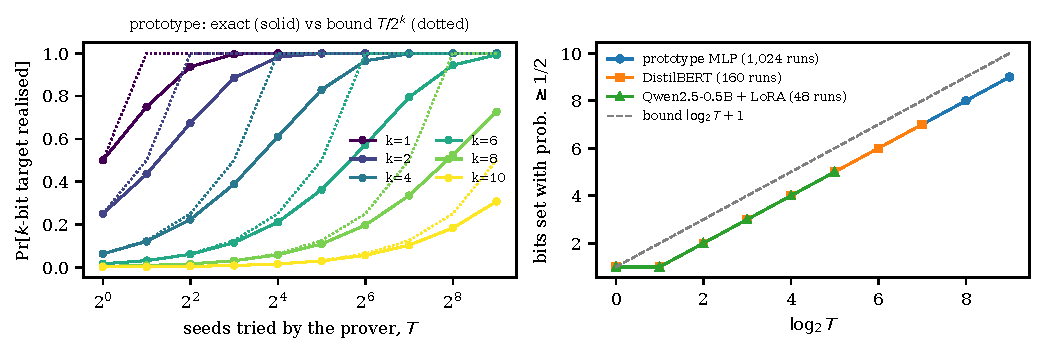
\includegraphics[width=0.8\textwidth]{fig/e3_grinding.pdf}
\caption{Seed grinding through a seed-accepting binding check. Left: prototype
(\EthreeN{} runs), exact probability of realising a random $k$-bit target (solid) and the
bound $T/2^k$ of Theorem~\ref{thm:grind} (dotted). Right: bits set with probability $\ge1/2$
for the prototype, DistilBERT (G1, \GOneN{} runs) and Qwen2.5-0.5B~+~LoRA (G4, \GFourN{}
runs); the three curves coincide where they overlap.}\label{fig:e3}
\end{figure*}

\subsection{Language-model scale (GPU)}

The prototype model is small. To check that binding by replay, grinding and detector
recall behave the same way for language models, we ran four experiments (G1--G4) on one consumer
GPU (NVIDIA \GPUname, 8\,GB; PyTorch \GPUtorch, CUDA \GPUcuda, Transformers \GPUtf) using
SST-2~\cite{socher2013sst}. The models were DistilBERT (\texttt{distilbert-base-uncased},
full fine-tuning) and Qwen2.5-0.5B with LoRA~\cite{hu2022lora} (rank 8 on the query and
value projections, sequence-classification head). Training ran in bf16 autocast, one
epoch, maximum length 64. A fifth experiment (G5) ran on a second machine, described below.

\paragraph{G2: exact replay}
Each configuration was trained three times from the same seed on 1,000 examples, both with
PyTorch's deterministic-algorithms mode and with default kernels (Table~\ref{tab:g2}). In
all four configurations the three runs produced bit-identical weights. Re-execution is
therefore a valid \textsf{BindFix}/\textsf{BindGrind} realisation for fine-tuning at this
scale on fixed hardware and software. Across machines it is not: G5 below re-executed nine
G3 runs on a second GPU with newer software, and none reproduced.

\begin{table}[t]
\centering\scriptsize
\caption{G2: replay of fine-tuning on one GPU (3 runs per row, same seed and data).}\label{tab:g2}
\resizebox{\columnwidth}{!}{\begin{tabular}{@{}llrcrr@{}}
\toprule
Model & kernels & trainable params & distinct hashes & max $|\Delta w|$ & train s\\
\midrule
\csname @@input\endcsname gen/tab_g2_rows.tex
\bottomrule
\end{tabular}}
\end{table}

\paragraph{G3: authorised-source poison at LLM scale}
An authorised source contributes $n$ dirty-label backdoor examples (negative sentences with
the trigger ``cf'' inserted, relabelled positive) to an 8,000-example committed set. Every
example carries a valid content-addressed Ed25519 receipt, so every provenance check
passes. We then measure the backdoor's attack success on triggered negative validation
sentences, and the recall of spectral signatures on DistilBERT's final-layer
\texttt{[CLS]} representation, flagging $1.5\varepsilon n_c$ items per class with
$\varepsilon=0.05$ (Table~\ref{tab:g3}).

\paragraph{Statistical treatment}
The replication unit is the training run (seed). Validation sentences within one run are not
independent replications of the model, so we report run-level values. For each run we give a
Wilson 95\% interval for its proportions, over $n=428$ triggered negative validation sentences
(attack success) and $n$ poisoned items (recall). We also give the attack success minus that of
the clean model with the same seed (\emph{baseline-adjusted}). With three seeds per condition
we report descriptive statistics only. A significance test over three runs would carry little
information (Table~\ref{tab:g3stats}).

The two curves cross. At 0.25--1\% poison, the detector finds 68--83\% of poisoned items on
average, but the backdoor has not taken hold after one epoch: mean baseline-adjusted attack
success stays between $-1$ and $+4$ points, with one run reaching $+9$ points at 1\%. At 2\%, the backdoor is effective in all three
runs, but unequally: baseline-adjusted attack success is $+\GthreeAdjHigh$ points on average,
ranging from $+\GthreeAdjHighMin$ to $+\GthreeAdjHighMax$. Mean recall falls to 25\%, with
wide per-run intervals.

Precision is the practical problem. The flag budget ($1.5\varepsilon n_c$ per class) sends
about \GthreeFPHigh{} clean examples per run to review at 2\% poison
(\GthreeFPRHigh\% of clean items). Only \GthreePrecHigh\% of flagged items are poisoned at 2\%,
and \GthreePrecLow\% at 0.25\%. A reviewer who inspects every flag therefore reads hundreds of
clean sentences per run, and still misses most of the poison where it matters. These are
results for one detector, one model and one trigger. They do not characterise poisoning
detection in general.

An auditor who holds a valid provenance record for this model holds no evidence about the
backdoor. This is Theorem~\ref{thm:content} measured on a pretrained transformer.
G5 below adds two detectors, a clean-data baseline and a higher poison level at GPU scale.

\begin{table}[t]
\centering\scriptsize
\caption{G3 summary: authorised-source backdoor poison, DistilBERT on SST-2 (3 seeds; mean
and range). Attack success over $n=428$ triggered negative sentences per run; clean accuracy
over $n=872$.}\label{tab:g3}
\resizebox{\columnwidth}{!}{\begin{tabular}{@{}rrclllr@{}}
\toprule
$n$ & rate & receipts & attack succ. & clean acc. & recall\phantom{x} & flagged\\
\midrule
\csname @@input\endcsname gen/tab_g3_rows.tex
\bottomrule
\end{tabular}}
\end{table}

\begin{table*}[t]
\centering\scriptsize
\caption{G3 per run (seeds 1, 2, 3). Attack success and recall in \% with Wilson 95\%
intervals; attack success over $n=428$ triggered negative sentences, recall over the $n$ poisoned
items. ``Adj.'': mean attack success minus the clean model's with the same seed, in percentage
points. FP: clean items flagged, mean over runs (rate over 8,000 clean items).}\label{tab:g3stats}
\begin{tabular}{@{}rp{6.2cm}rp{5.2cm}r@{}}
\toprule
$n$ & attack success per run [95\% CI] & adj. & recall per run [95\% CI] & FP (rate)\\
\midrule
\csname @@input\endcsname gen/tab_g3_stats_rows.tex
\bottomrule
\end{tabular}
\end{table*}

\paragraph{G5: three detectors and a second machine}
We added G5 in revision. It repeats the G3 protocol unchanged (same code, data, trigger,
seeds and training settings) at 0, 80, 160 and 320 poisoned items (0--3.8\%), and scores every
committed item with the three detectors of E2d, using the E2d flagging rules fixed before
the run. Unlike E2d, the detectors are applied to the trained model itself, as in G3. Because
the RTX~3070 machine was not available, G5 ran on a second machine: an NVIDIA \GFiveGPU{}
(\GFiveMem\,GB; PyTorch \GFiveTorch, CUDA \GFiveCuda, Python \GFivePy, Transformers \GFiveTf),
with deterministic kernels throughout, \GFiveTrainS\,s of training per run and at most
\GFivePeakGB\,GB of GPU memory. All \GFiveRuns{} runs completed, and \GFiveChecksOK{} of
\GFiveChecks{} automatic validity checks passed. The two that failed are the expected device
and the exact replay of G3, discussed next. Table~\ref{tab:g5} gives pooled recall and the
threshold-free AUROC within the target class, computed from the saved per-item scores.

\emph{Replay across machines.} Nine G5 runs (0, 80 and 160 poisoned items, seeds 1--3) are
exact re-executions of G3 runs. None reproduced G3's attack success, and \GFiveReplayAccEq{}
of \GFiveReplayN{} reproduced its clean accuracy. Below 2\% poison, attack success differed
by at most \GFiveReplayLowMaxDiff{} points; at 2\% it differed by up to \GFiveReplayMaxDiff{}
points for the same seed. GPU architecture and library versions changed together, so we
cannot attribute the difference to either. The practical consequence is clear: an auditor who
re-executes on a different stack does not obtain the trainer's model, so re-execution binding
needs a pinned hardware and software stack or a tolerance, and a tolerance enlarges
$\mathcal A_C$ (Theorem~\ref{thm:grind}).

\emph{Detection.} The qualitative results of G3 recur on the second machine. At 1\% poison
the backdoor has not taken hold, and the poison is easy to separate: AUROC
\GFiveSpecAucLow{} (spectral) and \GFiveLossAucLow{} (loss), with \GFiveSpecRecLow\% and
\GFiveLossRecLow\% recall within the flag budget, but only \GFiveSpecPrecLow\% precision. At
3.8\% the backdoor succeeds in every run (attack success at least \GFiveAsrHighMin\%), and
both detectors flag \GFiveRecHighTP{} of \GFiveHighN{} poisoned items; their AUROC
(\GFiveSpecAucHigh{} and \GFiveLossAucHigh) is at or below chance, so the poison looks
\emph{more} typical than clean data. Over the nine poisoned runs, recall falls as attack
success rises (Spearman $\rho=\GFiveRhoSpec$ for both; descriptive, since poison level drives
both; Fig.~\ref{fig:g5}). Activation clustering flagged a cluster in every run, including all three clean runs,
where it flagged \GFiveACCleanMin--\GFiveACCleanMax\% of clean items; its precision never
exceeded \GFiveACPrecMax\%. With this configuration it is not a usable detector here. These
results extend G3 to more detectors, a clean baseline and a higher poison rate; they use the
same model, data and trigger, so they say nothing about other models or attacks.

\begin{figure}[t]
\centering
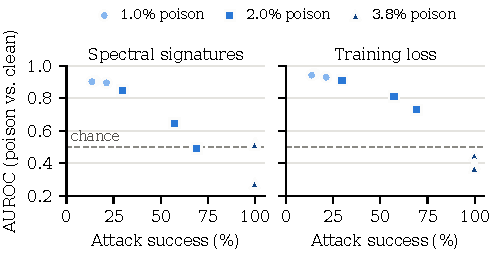
\includegraphics[width=\columnwidth]{fig/g5_detection.pdf}
\caption{G5: separability of poisoned from clean items (AUROC within the target class) against
the backdoor's attack success, one point per run. Detection is good only while the attack
fails; once the backdoor works in every run (3.8\% poison), both detectors are at or below
chance.}\label{fig:g5}
\end{figure}

\begin{table*}[t]
\centering\scriptsize
\caption{G5: three detectors on DistilBERT/SST-2 with authorised-source poison, run on a
second machine (\GFiveGPU; 3 seeds per row). Attack success: mean (range) over $n=428$
triggered negative sentences per run; clean accuracy over $n=872$. Recall: poisoned items
flagged out of all poisoned items over the 3 runs, flag budget $1.5\varepsilon n_c$ per class
($\varepsilon=0.05$, about 7.5\% of clean items by construction). AUROC: within the target
class, mean (range) over runs. Activation clustering: mean share of clean items flagged
(runs that flagged anything).}\label{tab:g5}
\begin{tabular}{@{}rrllllllr@{}}
\toprule
& & & & \multicolumn{2}{c}{spectral signatures} & \multicolumn{2}{c}{training loss} & act.\ clustering\\
$n$ & rate & attack succ.\ \% & clean acc.\ \% & recall & AUROC & recall & AUROC & clean FP\\
\midrule
\csname @@input\endcsname gen/tab_g5_rows.tex
\bottomrule
\end{tabular}
\end{table*}

\paragraph{G1 and G4: grinding at LLM scale}
We repeated E3 with \GOneN{} DistilBERT fine-tuning runs on a fixed 8,000-example committed set
(G1; \GOneTrainS\,s each; held-out accuracy $\GOneAcc\%\pm\GOneAccSd$; all \GOneDistinct{}
weight hashes distinct), and with \GFourN{} Qwen2.5-0.5B~+~LoRA runs on 2,000 examples
(G4; \GFourTrainS\,s each; accuracy $\GFourAcc\%\pm\GFourAccSd$). The probes, the disjoint
selection and evaluation seeds, and the exact analysis are the same as in E3. On the
selection seeds, \GOneSens\% (DistilBERT) and \GFourSens\% (Qwen~+~LoRA) of the 872 SST-2
validation sentences changed label across seeds.

The bits set with probability at least $1/2$ were exactly $\log_2T$ at every
$T\ge2$ for both models: \GOneBits{} bits at $T=\GOneTmax$ for DistilBERT and \GFourBits{}
bits at $T=\GFourTmax$ for Qwen~+~LoRA (Fig.~\ref{fig:e3}, right). This is the same curve as the
small prototype. In this setting, the channel's capacity is set by the number of training runs
the prover can afford, not by the model. Again the ground models were of ordinary quality:
\GOneChosenAcc\% against \GOneAllAcc\% for DistilBERT ($k=\GOneStK$, $T=\GOneStT$), and
\GFourChosenAcc\% against \GFourAllAcc\% for Qwen~+~LoRA ($k=\GFourStK$, $T=\GFourStT$).
At the measured training times, setting 7 chosen bits of a DistilBERT fine-tune takes under an hour
on a laptop GPU.

\subsection{Cost of record-level mechanisms (E4)}

\begin{table}[t]
\centering\scriptsize
\caption{Cost of record-level mechanisms on one CPU core (1\,KiB items). Per-item costs in
$\mu$s. Merkle root over all items in ms.}\label{tab:e4}
\setlength{\tabcolsep}{4.5pt}\begin{tabular}{@{}rrrrrrr@{}}
\toprule
items & hash & sign rcpt & verify rcpt & root (ms) & proof len & receipts (MB)\\
\midrule
\csname @@input\endcsname gen/tab_e4_rows.tex 
\bottomrule
\end{tabular}
\end{table}

Table~\ref{tab:e4} shows that hashing, receipts and commitments cost microseconds per item
and scale linearly. At the measured rate, verifying receipts for a corpus of $10^9$ documents would take about
\EfourVerifyHours{} core-hours, and the work is trivially parallel. The dominant cost of any
configuration that includes binding is binding itself. Exact re-execution doubles training,
and proof systems cost much more~\cite{abbaszadeh2024zkpot,liao2026verilora}.

\subsection{Published systems through the model (E1)}

Table~\ref{tab:e1} maps published systems to the model and reads off the goals they support.
The mapping uses each paper's own description of its mechanisms and trust assumptions. For
Atlas and VAMP we read the threat-model sections. For the others the mapping is from the
abstract and is marked as such.

\begin{table*}[t]
\centering\scriptsize
\caption{Published systems mapped to the model. ``Profile'' is the closest adversary profile
implied by the paper's threat model. Mechanisms marked $\tau$ are realised by trusted
hardware and are lost under \textsf{AdvTEE}.}\label{tab:e1}
\begin{tabular}{@{}p{2.3cm}p{3.6cm}p{2.1cm}p{4.6cm}p{3.6cm}@{}}
\toprule
System & Mechanisms (as described) & Profile & Goals supported per the model & Remark\\
\midrule
Atlas~\cite{spoczynski2025atlas} (threat model read) & TEE attestation of every transformation and its inputs; transparency log & MLaaS provider, hubs, producers untrusted $\approx$ full & With CPU-only TEEs and GPU training outside them (the paper's own limitation): $G_{\mathrm{compl}}$ only. With attested training (Bind under $\tau$): $G_{\mathrm{bind}}$, $G_{\mathrm{auth}}$ via AC+AT+$\beta$ & Dataset benignity out of scope, consistent with Thm.~\ref{thm:content}\\
Laminator~\cite{duddu2025laminator} (abstract) & Hardware-attested property cards for data, training, inference & full & Attested claims only under $\tau$; under full+tee none remain & No content claim beyond attested properties\\
VAMP~\cite{stokes2021prevent} (threat model read) & Signed manifests over datasets, software, models (WitSrc) & Infrastructure trusted $\approx$ trans-only & $G_{\mathrm{auth}}$ for filter-only pipelines; no $G_{\mathrm{zero}}$ & Title claims poisoning \emph{prevention}; holds for unauthorised modification only (Thm.~\ref{thm:content}.1)\\
PoL~\cite{jia2021pol} & Spot-check re-execution with tolerance, prover-chosen randomness & exec-only & $G_{\mathrm{bind}}$ up to spoofing~\cite{fang2023pol}; not $G_{\mathrm{noinf}}$ (BindGrind) & Tolerance enlarges the grinding set (Thm.~\ref{thm:grind})\\
VeriLoRA~\cite{liao2026verilora} (protocol sections read) & ZK proof of every LoRA step (forward, backward, update); initial weights committed as part of the witness & exec-only & $G_{\mathrm{bind}}$ as \textsf{BindGrind}: the paper does not fix mini-batch sampling or initialisation randomness by the verifier, so not $G_{\mathrm{noinf}}$; no dataset commitment is described, so binding to a record needs one; no lineage without WitSrc or attestation & Combine with a beacon-derived seed and data commitment to obtain \textsf{BindFix}\\
Kaizen zkPoT~\cite{abbaszadeh2024zkpot} (protocol sections read) & ZK proof of every training iteration over a Merkle-committed dataset; prover commits the initial weights; batch order from a public pseudorandom permutation key & exec-only & $G_{\mathrm{bind}}$ as \textsf{BindGrind}: the prover commits its own initial weights, the protocol does not require the permutation key to be fixed by the verifier after the data commitment, and the number of proved iterations need not be fixed in advance, so not $G_{\mathrm{noinf}}$; no lineage without WitSrc or attestation & Seed rejection sampling against zkPoTs demonstrated by~\cite{tan2025zkpot}\\
Optimum-vicinity zkPoT~\cite{tan2025zkpot} (full text read) & ZK proof that the released model is within $\epsilon$ of the optimum of an $L_2$-regularised convex loss on the committed data & exec-only & $G_{\mathrm{bind}}$ with $\mathcal A_C$ an $\epsilon$-ball, independent of training randomness; influence bounded geometrically rather than by $T$ & Logistic regression and SVMs; no lineage or content claim\\
AuditableLLM~\cite{li2025auditablellm} (abstract) & Hash-chained audit trail of updates & exec-only & Store integrity ($P_1$) only; no pipeline goal & ``Verifiable integrity'' is of the log, not of the training\\
Mehammed et al.~\cite{mehammed2025fl} (abstract) & Permissioned ledger, update audit, zk-SNARK of client summaries & full (clients untrusted) & $P_1,P_2,P_8$; no binding of client training, so no pipeline goal & Ledger contributes $P_8$ (Prop.~\ref{prop:ledger})\\
\bottomrule
\end{tabular}
\end{table*}

The pattern is consistent. Systems that state a narrow threat model (Atlas and VAMP, which
trust the verification or training infrastructure) make claims that the model supports
within that model. The model's value is that it says what changes when the trust assumption
does not hold. Claims phrased as preventing poisoning, or as verifiable integrity of
training, hold only for the narrower properties the model identifies.

% ---------------------------------------------------------------
\section{Literature Search Method}\label{sec:lit}
% ---------------------------------------------------------------

The systematisation in Section~\ref{sec:sok} rests on a structured search. We report it
in PRISMA~2020 terms~\cite{page2021prisma} and state plainly which stages are incomplete.

\paragraph{Search}
On 25~October~2026 we ran 12 query strings against OpenAlex. The strings cover provenance
and lineage capture, ledgers, transparency logs, trusted execution, proofs of learning,
zero-knowledge training proofs, data-use auditing and poisoning defences. We retrieved
the first 25--100 results per string (24 result pages in total, depth by string as
recorded in the artefact). This produced 594 records. A version-aware deduplication kept
the peer-reviewed version of each work and recorded all its DOIs, which removed 43
duplicates.

\paragraph{Eligibility}
Inclusion required (I1) an ML or AI training pipeline, (I2) a mechanism for provenance,
integrity or verification of training data or training computation, and (I3) peer review.
Exclusion codes covered: no ML context (E1); inference-output provenance only (E2);
document types outside the protocol (E3); poisoning work without a provenance or
verification component (E5); and preprint-only works (E7). E7 works were kept in a
separate positioning list and are not cited as evidence.

\paragraph{Screening}
A rule-based pre-screen excluded 248 of 551 records: 135 preprint-only, 90 without ML or
provenance terms, and 23 by document type. An audit of 92 rule exclusions by title found
2 false exclusions, which were restored. Title-and-abstract screening of the remaining 303
records was carried out by an AI assistant (Claude) applying the written protocol. Every
decision is logged with a reason code and labelled as an AI decision requiring human
verification. It excluded 154 records and passed 149 (55 marked \emph{unsure}). Nine further
records came from citation chasing. That leaves 158 records for full-text assessment.

\paragraph{Status and limits}
\pending{Full-text screening of the 158 records, a human second screener with reported
agreement ($\kappa$) on at least a 20\% sample, and searches of Scopus, Web of Science,
IEEE~Xplore and the ACM Digital Library are not yet complete. Until they are, the search
is a structured mapping, not a systematic review.} A known-item check found 8 of 17 seed
papers that the authors had identified beforehand. The misses include Atlas and Sigstore,
which is why the database searches above are required before submission. The screening log,
queries and raw result pages are part of the artefact.

% ---------------------------------------------------------------
\section{Discussion}\label{sec:discussion}
% ---------------------------------------------------------------

\subsection{What an auditor may conclude}

\begin{figure}[t]
\centering
\resizebox{\columnwidth}{!}{% Fig.: what an auditor may conclude (Discussion), column width
\begin{tikzpicture}[font=\sffamily\scriptsize, >={Stealth[length=1.6mm]},
  q/.style={draw=black!55, fill=black!4, rounded corners=2pt, text width=24mm, align=center,
            inner sep=2pt, minimum height=13mm,
            execute at begin node={\hyphenpenalty=10000\exhyphenpenalty=10000}},
  a/.style={draw=black!30, fill=white, rounded corners=2pt, text width=47mm, align=flush left,
            inner sep=2.5pt, minimum height=13mm,
            execute at begin node={\hyphenpenalty=10000\exhyphenpenalty=10000}},
  fl/.style={->, black!65, line width=0.6pt}]
\newcommand{\Y}{\textcolor{okgreen}{\textbf{yes}}}
\newcommand{\N}{\textcolor{advorange}{\textbf{no}}}
\def\dy{1.65}
\node[q] (q1) at (0,0)      {\textbf{1} Is the trainer trusted?};
\node[q] (q2) at (0,-\dy)   {\textbf{2} Does the verifier fix the seed after the data commitment?};
\node[q] (q3) at (0,-2*\dy) {\textbf{3} Is there an authenticated route from sources to training?};
\node[q] (q4) at (0,-3*\dy) {\textbf{4} Is the model free of poison?};
\node[a, right=3mm of q1] (a1) {\Y: attested capture binds the model to its record; no proof of training needed.\\
  \N: binding (exact replay or a proof of training) is required. \hfill\textcolor{black!55}{Thm.~\ref{thm:bind}}};
\node[a, right=3mm of q2] (a2) {\Y: no prover influence, if replay is exact on a pinned stack.\\
  \N: up to $\log_2 T$ chosen bits for $T$ runs. \hfill\textcolor{black!55}{Thms.~\ref{thm:noinf},~\ref{thm:grind}; G2, G5}};
\node[a, right=3mm of q3] (a3) {\Y, with binding: lineage holds via source witnesses or attested capture and transform; stage types must be declared. \N: no lineage claim. \hfill\textcolor{black!55}{Thm.~\ref{thm:auth}, Cor.~\ref{cor:launder}}};
\node[a, right=3mm of q4, draw=advorange, fill=advorange!7] (a4) {Never certified. At best: every poisoned item used was missed by the detector, worth its recall, which collapsed once the backdoor worked. \hfill\textcolor{black!55}{Thm.~\ref{thm:content}; G3, G5}};
\foreach \i [count=\j from 2] in {1,2,3} \draw[fl] (q\i) -- (q\j);
\foreach \i in {1,...,4} \draw[fl] (q\i) -- (a\i);
\end{tikzpicture}
}
\caption{Four questions an auditor should answer before accepting a claim about a released
model, and what the theorems and experiments say for each answer.}
\label{fig:auditor}
\end{figure}

Table~\ref{tab:minimal} can be read as a checklist, and Fig.~\ref{fig:auditor} condenses it
into four questions. Before accepting a claim about a
released model, an auditor should establish three things:
\begin{enumerate}
\item Who is trusted: which profile applies.
\item Which mechanisms were actually deployed and verified.
\item Which goal the claim corresponds to.
\end{enumerate}
Two examples show how this works.

A cloud provider's attested data pipeline without binding (\textsf{AttCap}, \textsf{AttTrans}
under the full adversary) supports no claim about the released model. It does support the
record-level claim $G_{\mathrm{compl}}$.

A signed-manifest scheme with a trusted training infrastructure (the trans-only or cap-only
profiles) does support lineage for filter-only pipelines, but not the absence of poison.

\subsection{Answers to five design questions}

\paragraph{Binding}
Binding is required whenever the trainer is not trusted, and no amount of witnessing or
attestation of earlier stages substitutes for it (Theorem~\ref{thm:bind}). If binding is
used, its randomness must be fixed after commitment (Theorems~\ref{thm:noinf}
and~\ref{thm:grind}). Exact re-execution is a valid binding only where training is
bit-reproducible. Section~\ref{sec:eval} measures when it is.

\paragraph{Witnessing}
Source receipts must be content-addressed (split view, Section~\ref{sec:eval}). Source
witnessing and input witnessing answer different questions, lineage and completeness. Each
fails under collusion, so witnesses should be organisationally independent of the operator
they observe.

\paragraph{Synthetic data}
Generative stages need an attested transform even on the witness route, and stage types
must be declared and authenticated (Corollary~\ref{cor:launder}). Lineage of synthetic data
is recursive: the generator is itself a model whose provenance matters. Our model treats it
as an authorised but possibly poisoned source (\textsf{AdvGen}).

\paragraph{Blockchain versus transparency logs}
For every goal we study, a witnessed transparency log is sufficient as the record store.
A ledger adds inclusion liveness (Proposition~\ref{prop:ledger}). We find no support for
the claim that a blockchain makes training records complete or truthful. Those properties
are decided upstream of the store.

\paragraph{Poisoning}
Provenance cannot certify that a model is poison-free (Theorem~\ref{thm:content}). It can
make a detector's verdict \emph{transfer} to the released model, which is what binding and
completeness contribute. The resulting claim is only as strong as the detector's recall.
In our experiments, recall was weakest exactly where the poison worked. The prototype's detector flagged at most a quarter of the planted items. On DistilBERT, recall fell from 68--83\% at the lower, ineffective poison rates to 25\% at the 2\% rate where the backdoor took hold (Section~\ref{sec:eval}). Any
certification scheme that reports provenance without detector recall overstates its
assurance.

\subsection{Open problems}

\begin{enumerate}
\item \emph{Binding at pre-training scale.} Zero-knowledge binding now reaches LoRA
  fine-tuning~\cite{liao2026verilora}, but not full pre-training. Exact re-execution
  doubles the cost and requires determinism. Spot-check proofs of learning admit spoofing
  under tolerance~\cite{fang2023pol}.
\item \emph{Tolerance as a grinding channel.} Theorem~\ref{thm:grind} bounds influence by the
  number of accepted trajectories. For tolerance-based verifiers that number is not
  characterised. Optimum vicinity~\cite{tan2025zkpot} closes the channel for convex
  objectives; for non-convex LLM training it remains open.
\item \emph{Attested accelerators.} The attestation routes assume that the relevant stages run
  in TEEs. Atlas notes that GPUs lack equivalent protection~\cite{spoczynski2025atlas}.
\item \emph{Detector guarantees.} $G_{\mathrm{content}}$ is parameterised by recall. Certified
  recall bounds for poisoning detectors at LLM scale are lacking.
\item \emph{Confidential verifiability ($P_7$).} All our mechanisms reveal the record to the
  auditor. Combining them with confidentiality of training data is open.
\item \emph{Composition across model generations.} Fine-tuning chains and synthetic data make
  provenance recursive. The model covers one training run.
\end{enumerate}

\subsection{Limitations}

\paragraph{Model}
The model has five abstractions:
\begin{itemize}
\item Items are atomic and content-identified.
\item Each mechanism is all-or-nothing.
\item A single training run is modelled.
\item Detectors are abstracted to an examined set and a miss set, with no budget or base
  rate.
\item Correlated compromise is captured \emph{across} trust anchors (any subset of
  capabilities), but not \emph{within} a mechanism class, such as one corrupt witness among
  several.
\end{itemize}
Table~\ref{tab:scope} lists which training practices fall inside the abstraction. The
model's results are exact for the model only. Their relevance to real systems rests on the
validation in Section~\ref{sec:eval}.

\paragraph{Prototype}
The prototype trains a small bag-of-words network on 2,000 reviews. It simulates trusted
execution with key isolation rather than real enclaves, so it validates the logic of
attestation-based checks, not any hardware. It compares three detectors on one small model. Poisoning at GPU scale was
measured on one model (DistilBERT), one dirty-label trigger and three seeds per condition,
with one detector in G3 and three in G5, so it is reported descriptively. G5 ran on a second,
smaller GPU because the first was unavailable; its qualitative results match G3, but its runs
did not replay G3's bit for bit. Bit-exact replay therefore holds on a fixed stack only, and
we changed GPU and library versions together, so we cannot say which change breaks it. The
GPU experiments cover fine-tuning, not pre-training.
Their seed counts (160 and 48) limit the largest $T$ we could test to 128 and 32.

\paragraph{Literature}
The literature search used one database, title-and-abstract screening was performed by an
AI assistant, and full-text assessment is pending (Section~\ref{sec:lit}). The case-study
mapping relies partly on abstracts.

\paragraph{Proofs}
The proofs are by hand. They are backed by two independent exhaustive decision procedures
for the six profiles, and by a third, vectorised checker over all 128 adversary subsets. They
are not mechanised in a proof assistant. Proposition~\ref{prop:ledger} and the composition
remark of Section~\ref{sec:scope} are argued, not proved.


\section{Artefact, Data, Ethics and AI-Use Statement}\label{sec:artefact}
\paragraph{Artefact}
The artefact contains:
\begin{itemize}
\item the Alloy models, the sweep, the independent checker, the adversary-lattice checker and
  their raw outputs;
\item the prototype and every experiment script with raw and processed results;
\item the GPU kit with its logs;
\item the G5 kit, its logs and per-item detector scores;
\item the literature-search queries, raw result pages and screening log;
\item SHA-256 manifests and a reproducibility guide that regenerates every table and figure.
\end{itemize}
The artefact is archived on Zenodo, version~1.1:
\url{https://doi.org/10.5281/zenodo.24420107} (all versions:
\url{https://doi.org/10.5281/zenodo.24317966}). Code is released under the MIT licence and
results, data and documentation under CC~BY~4.0. A working copy is maintained at
\url{https://github.com/waqas6755/what-can-provenance-prove}. The archive holds a reproducibility
guide that maps each table and figure to the script and raw file that produce it, and SHA-256
checksums of its files.

\paragraph{Data, models and licences}
The prototype uses the polarity dataset v2.0~\cite{pang2004sentimental}, as distributed by
NLTK. The GPU experiments use SST-2~\cite{socher2013sst} from the GLUE distribution, with
\texttt{distilbert-base-uncased} and \texttt{Qwen/Qwen2.5-0.5B} from the Hugging Face Hub. No
personal data is processed. Both models are released under the Apache~2.0 licence. Neither the
polarity dataset nor the Stanford Sentiment Treebank states a licence: the polarity dataset's
distribution page asks users to cite its version number, and the GLUE distribution refers users to
the licence of each source dataset. We use both datasets unmodified, for research only, and do not
redistribute them; the artefact gives download instructions instead.

\paragraph{Dual use and disclosure}
The attacks we implement (split-view delivery, laundering, seed grinding, authorised-source
backdoors) are either already published or follow directly from the model. They are run only
against our own prototype and public models. The grinding result points to a simple
mitigation, a beacon-fixed seed, which we recommend to builders of proof-of-training systems.
No third-party system was attacked.

\paragraph{AI assistance}
An AI assistant (Claude, Anthropic) was used to:
\begin{itemize}
\item write experiment and analysis code;
\item run the model checker and the experiments in the cloud environment;
\item draft and revise text;
\item perform title-and-abstract screening.
\end{itemize}
The AI screening decisions are labelled as such in the released log. They have not been
verified by a human screener, and they are not reported as independent human screening. The
authors are responsible for verifying the code, results and proofs, and for all claims.
\pending{State which verification the authors have personally carried out.} \pending{Check this statement against the journal's current AI-use policy before
submission.}

\section{Conclusion}
We separate the conclusions by the kind of evidence behind them.

\paragraph{Proved within the model}
\begin{itemize}
\item Computation binding is necessary exactly when the trainer is untrusted.
\item Lineage has two routes with disjoint trust anchors.
\item Generative pipelines need authenticated stage types.
\item A seed-accepting binding check leaks at most $\log_2T$ bits for $T$ evaluated accepted
  outputs.
\item No mechanism set certifies the absence of poison; the strongest claim is conditional on
  a detector.
\item Attested capture and input witnessing are interchangeable for record completeness.
\end{itemize}
These statements hold for every subset of adversary capabilities. They are exact for the
abstract single-run model of Section~\ref{sec:model}, within the scope of
Table~\ref{tab:scope}.

\paragraph{Observed in our experiments}
\begin{itemize}
\item A prototype with real cryptography and simulated trusted execution matched the model
  on all 9,216 instances.
\item Seed grinding reached $\log_2T$ bits on a small model, on DistilBERT and on Qwen
  2.5-0.5B~+~LoRA.
\item Fine-tuning replayed bit for bit on one machine, but not on a second machine with a
  different GPU and newer libraries.
\item One spectral-signature detector lost most of its recall exactly where an
  authorised-source backdoor became effective, at low precision.
\item On the prototype, three detectors, including a loss score and activation clustering,
  showed the same pattern or found nothing.
\item At GPU scale, spectral and loss detectors separated poison well at 1\% poison and fell
  to chance at 3.8\%, where the backdoor always worked; activation clustering flagged about a
  quarter of clean data even with no poison.
\end{itemize}

\paragraph{From the literature}
The surveyed systems make claims that hold within their own trust assumptions. Claims of
poisoning prevention, or of verifiable integrity of training, hold only for the narrower
properties identified in Table~\ref{tab:e1}. This conclusion rests on a structured mapping,
not yet a systematic review (Section~\ref{sec:lit}).

\paragraph{Design rules and future work}
\begin{itemize}
\item Bind the computation whenever the trainer is untrusted, with randomness fixed after
  commitment.
\item Use content-addressed receipts and authenticated stage types.
\item Diversify trust anchors.
\item Report detector recall and precision alongside any content claim.
\item Use a ledger only where censorship-resistant inclusion is itself a requirement.
\end{itemize}
Future work includes binding at pre-training scale, replay across hardware stacks (which
failed in our one cross-machine test), multi-stage and
multi-parent model lineages, real enclave deployments, and detectors with guaranteed recall.

\bibliographystyle{IEEEtran}
\bibliography{refs}

\ifproofsinpaper
\appendices
% ---------------------------------------------------------------
\section{Proofs}\label{app:proofs}
% ---------------------------------------------------------------

Throughout, an execution is written $E=(\mathcal I,\{v_i\}_{i\in\mathcal I},g)$. Here
$v_i\in\{0,1\}^{11}$ records the membership of item $i$ in
$D,S,F,C,U,\hat S,\hat D,\hat F,B,M,X$, and $g$ collects the global Booleans: $\alpha$,
$\mu$, $\mathit{gen}$, $\mathit{gs}$, and whether the detector is perfect. We write
$i\in D$ for $v_i[D]=1$. A \emph{counterexample} to $\mu\models_{\alpha,\mathit{gen}}G$ is an
admissible, accepted execution that violates $G$. In every construction below, $X$ is set
equal to $C$ whenever $\textsf{Detector}\in\mu$ and $\tau$ hold, as $\Phi_8$ requires, and
the listed items are not in $B$ unless stated. We leave $X$ out of the listed vectors.

\subsection*{Proof of Lemma~\ref{lem:sep} (Separability)}

\emph{Form of the constraints.}
Each set equation or inclusion between sets in $\Phi$, $\mathrm A$ and the goals is a
universally quantified per-item statement. For example, $C\subseteq\hat D\cup\hat S$ is
$\forall i.\ i\in C\Rightarrow(i\in\hat D\vee i\in\hat S)$, and $U=C$ is
$\forall i.\ i\in U\Leftrightarrow i\in C$. Emptiness ($S=\emptyset$) and disjointness
($D\cap S=\emptyset$) are also per-item. Each premise of an implication in $\Phi$ or
$\mathrm A$ (``$\textsf{AdvTrans}\notin\alpha$'', ``$\beta$'', ``$\mathit{gen}$'') mentions
only global Booleans. Hence each constraint has the form
$\psi(g)\Rightarrow\forall i.\ \varphi(v_i,g)$, which equals
$\forall i.\ (\psi(g)\Rightarrow\varphi(v_i,g))$ whenever $\mathcal I\neq\emptyset$.
Two constraints mention only $g$:
$\mathit{gs}\Rightarrow(\textsf{AdvExec}\in\alpha\wedge\textsf{BindFix}\notin\mu)$ in
$\Phi_6$, and the conjunct $\neg\mathit{gs}$ of $G_{\mathrm{noinf}}$. Write the admissible,
accepted executions as those satisfying
$\chi_\Phi(g)\wedge\forall i.\ \varphi_\Phi(v_i,g)$, and each goal as
$\chi_G(g)\wedge\forall i.\ \varphi_G(v_i,g)$.

\emph{The zero vector.}
Let $\mathbf 0$ be the vector with every membership $0$. Every per-item constraint holds
at $\mathbf 0$. Every inclusion $P\subseteq Q$ holds because $i\notin P$. Every equation
$P=Q$ holds because both sides are false. Every emptiness and disjointness condition holds
trivially. Each $\varphi_G$ holds at $\mathbf 0$ for the same reasons. (This side condition
is also asserted mechanically by our independent checker.)

\emph{Reduction.}
($\Leftarrow$) Let $E$ be a counterexample over $\mathcal I$. Then $\chi_\Phi(g)$ holds,
$\varphi_\Phi(v_i,g)$ holds for every $i$, and either $\chi_G(g)$ fails or
$\varphi_G(v_{i_0},g)$ fails for some $i_0$. In the first case, the one-item execution
$(\{j\},v_j{=}\mathbf 0,g)$ is admissible, accepted and violates $\chi_G$. In the second,
the restriction $(\{i_0\},v_{i_0},g)$ is admissible and accepted (its only item satisfied
every per-item constraint in $E$), and it violates $\varphi_G$. Either way there is a
one-item counterexample.
($\Rightarrow$) Given a one-item counterexample $(\{i_0\},v_{i_0},g)$ and any universe
$\mathcal I\ni i_0$, assign $\mathbf 0$ to every other item. The new items satisfy every
per-item constraint and goal, so the extended execution is admissible, accepted and still
violating. Hence a counterexample exists over some universe iff one exists over a single
item. \qed

\emph{The empty universe.} If $\mathcal I=\emptyset$, only the global conditions $\chi$
remain. Any counterexample there violates some $\chi_G$. It is then reproduced by the
one-item execution with the zero vector, which is admissible and accepted. So restricting
the check to one item loses nothing.

\emph{When the lemma fails.} The lemma uses two facts: every constraint is a per-item
universal statement or a global condition, and the zero vector satisfies every per-item
constraint. A constraint that relates different items breaks the first fact. Examples are a
cardinality bound (``at most $n$ items are flagged'', a detector \emph{budget}), a ratio (``at
most $\varepsilon$ of $C$ is poisoned''), or a relation between runs (``$C_j$ contains
$M_{j-1}$''). Extensions with such constraints need bounded model checking, or a new argument.
This is why detector budgets and poison rates appear in our experiments and not in the
model.

\subsection*{Proof of Proposition~\ref{prop:mono} (Monotonicity)}

Let $\mu\subseteq\mu'$, and let $E'$ be a counterexample for $\mu'$. We build a
counterexample for $\mu$. Adding a mechanism has three effects. It adds acceptance
conditions ($\mathrm A_1$--$\mathrm A_4$). It strengthens admissibility constraints
($\Phi_3$--$\Phi_5$ only gain premises that make them apply). And it can enlarge $X$ from
$\emptyset$ to $C$ ($\Phi_8$). Take $E$ equal to $E'$ except that $X$ is recomputed by
$\Phi_8$ for $\mu$, and $\mathit{gs}$ is unchanged. Every constraint that applies under
$\mu$ also applies under $\mu'$, so $E$ is admissible and accepted. The one exception is
$\Phi_6$'s $\mathit{gs}$ clause, which is weaker under $\mu$ because $\mu$ has no more
\textsf{BindFix} than $\mu'$. $X$ occurs in the goals only on the right of an inclusion
($G_{\mathrm{content}}$), and $X_E\subseteq X_{E'}$. So any goal violated by $E'$ is
violated by $E$. \qed

\subsection*{Proof of Theorem~\ref{thm:bind} (Binding)}

\emph{Sufficiency.} $\beta$ with $(\mathrm A_1)$ gives $U=C$. If
$\textsf{AdvExec}\notin\alpha$, then $U=F$ by $\Phi_6$. Then $\textsf{AdvCap}\notin\alpha$
or $(\textsf{AttCap}\in\mu\wedge\tau)$ gives $C=F=U$ by $\Phi_5$.

\emph{Necessity.} Let $\textsf{AdvExec}\in\alpha$ and $\neg\beta$. Take one item with
$v=\{U\}$ (only $U$ set). No constraint of $\Phi$ mentions $U$ except $\Phi_6$, whose
premise fails. $(\mathrm A_1)$ is vacuous; $(\mathrm A_2)$ and $(\mathrm A_4)$ concern
$C=\emptyset$; $(\mathrm A_3)$ holds because $\hat F=F=\emptyset$. So the execution is
accepted, and $U\neq C$. Now let $\textsf{AdvExec}\notin\alpha$, $\textsf{AdvCap}\in\alpha$,
$\neg\beta$, and $\textsf{AttCap}\notin\mu$ or $\neg\tau$. Take $v=\{D,\hat D,C\}$. The item
is delivered and witnessed, but filtered out by an honest transform and re-added by a
corrupt capture. $F=U=\emptyset$, $C=\{i\}$; $(\mathrm A_2)$ holds because $i\in\hat D$, and
$(\mathrm A_3)$ holds because $\hat F=\emptyset$. Hence $U\neq C$. \qed

\subsection*{Proof of Theorem~\ref{thm:auth} (Lineage)}

Fix the full adversary, so $\tau$ holds, $\textsf{AdvWit}\notin\alpha$ and
$\hat D=D,\hat F=F$.

\emph{Sufficiency.} By $(\mathrm A_1)$, $U=C$.
(a) $\textsf{WitSrc}$, $\neg\mathit{gen}$: $(\mathrm A_2)$ gives $C\subseteq D\cup\hat S$,
and $\hat S=\emptyset$ by $\Phi_1$. Hence $U\subseteq D$.
(b) $\textsf{WitSrc}\wedge\textsf{AttTrans}$: $\hat S=S$ by $\Phi_4$, so
$U=C\subseteq D\cup S$.
(c) $\textsf{AttCap}\wedge\textsf{AttTrans}$: $C=F$ by $\Phi_5$ and $F\subseteq D\cup S$ by
$\Phi_3$, so $U\subseteq D\cup S$.

\emph{Necessity.} By monotonicity it suffices to refute the maximal mechanism sets outside
the stated condition. Each counterexample below has one item $x$ with $x\notin D\cup S$.
\begin{itemize}
\item $\neg\beta$ (all other mechanisms present): $v=\{U\}$, as in Theorem~\ref{thm:bind}.
\item $\beta$, no \textsf{WitSrc}, no \textsf{AttTrans}: $v=\{F,C,U,\hat F\}$. $\Phi_3$ does not
  apply ($\textsf{AdvTrans}$, no attestation), so $F$ is unconstrained.
  \textsf{AttCap} gives $C=F$, and $(\mathrm A_3)$ holds because $\hat F=F\subseteq C$.
\item $\beta$, no \textsf{WitSrc}, no \textsf{AttCap}: $v=\{C,U\}$. $\Phi_5$ does not apply,
  so $C$ is unconstrained. $F=\emptyset$ satisfies $\Phi_3$, and $(\mathrm A_3)$ is vacuous.
\item $\mathit{gen}$, $\beta$, \textsf{WitSrc}, no \textsf{AttTrans} (\textsf{AttCap},
  \textsf{WitIn}, \textsf{Detector} present): $v=\{F,C,U,\hat F,\hat S\}$. $\Phi_4$ does not
  apply, so $\hat S$ is unconstrained (the transform \emph{launders} $x$ as synthetic).
  $(\mathrm A_2)$ holds because $x\in\hat S$.
\end{itemize}
In every case $x\notin B$, so $(\mathrm A_4)$ holds, and $U\not\subseteq D\cup S$.

\emph{Colluding witnesses (full+wit).} $\Phi_7$ no longer applies, so $\hat D$ and
$\hat F$ are unconstrained. Every mechanism set without both \textsf{AttCap} and
\textsf{AttTrans} then fails. Without \textsf{AttTrans}, use $v=\{F,C,U,\hat D\}$.
Without \textsf{AttCap}, use $v=\{C,U,\hat D\}$. Proof (c) does not use witnesses, so the
attestation route still holds.

\emph{Broken attestation (full+tee).} $\tau$ fails, so $\Phi_3$--$\Phi_5$ never apply
through attestation, and $\hat S$ is unconstrained whenever $\mathit{gen}$ holds. For
filter-only pipelines, (a) still applies. For generative ones, the laundering instance
refutes every mechanism set. \qed

\subsection*{Proof of Corollary~\ref{cor:launder}}

Drop $\neg\mathit{gen}\Rightarrow\hat S=\emptyset$. Then the laundering instance of the last
bullet above is admissible for filter-only pipelines too. So
$\{\textsf{BindFix},\textsf{BindGrind},\textsf{WitSrc},\textsf{WitIn},\textsf{AttCap},\textsf{Detector}\}$
fails $G_{\mathrm{auth}}$. \qed

\subsection*{Proof of Theorem~\ref{thm:noinf} (Influence)}

If $\textsf{BindFix}\in\mu$, then $\Phi_6$ forces $\neg\mathit{gs}$, and $\beta$ gives
$U=C$. If $\textsf{BindFix}\notin\mu$, the execution with every item $\mathbf 0$ and
$\mathit{gs}$ true is admissible ($\textsf{AdvExec}\in\alpha$) and accepted, and it
violates $G_{\mathrm{noinf}}$. \qed

\subsection*{Proof of Theorem~\ref{thm:grind} (Grinding bound)}

Write the candidates as $\Sigma=\{M_1,\dots,M_T\}\subseteq\mathcal A_C$. By assumption
they are generated independently of $K$, so $(C,\Sigma)$ is independent of $K$. Given
$(C,\Sigma)$, the released $M$ is a function of the index $j^\ast$ with $M=M_{j^\ast}$.
Hence $H(M\mid C,\Sigma)\le H(j^\ast)\le\log_2T$. Since $I(K;M\mid C,\Sigma)\le
H(M\mid C,\Sigma)$, this gives $I(K;M\mid C,\Sigma)\le\log_2T$.

For the second claim, let $\pi(M)\in\{0,1\}^k$ be the behaviour pattern the adversary
targets. Given $(C,\Sigma)$, $\pi(M)$ takes values in the set
$P_{C,\Sigma}=\{\pi(M_j)\}_j$, which has at most $T$ elements. For $K$ uniform and
independent of $(C,\Sigma)$,
\[
\Pr[\pi(M)=K]\le\Pr[K\in P_{C,\Sigma}]=\mathbb E\,|P_{C,\Sigma}|/2^k\le T/2^k.
\]
The same bound holds if the prover evaluates the candidates one at a time and stops at the
first match. The patterns it can reach are still those of at most $T$ candidates drawn
independently of $K$. Success probability at least $1/2$ therefore requires $T\ge2^{k-1}$.

Under \textsf{BindFix}, the verifier recomputes the seed from the committed record and a
beacon released after commitment, and replays exactly. Then
$\mathcal A_C=\{\mathrm{Train}(C,s_{\mathrm{fix}})\}$, so $T=1$.

\emph{Scope of the proof.} The bound depends only on $|\Sigma|$. It does not assume that
candidates are distinct seeds, that training is deterministic, or that $\mathcal A_C$ is
small. Nondeterminism and tolerance enter only through the size of $\mathcal A_C$, and so
through how large a $T$ the prover can obtain. \qed

\subsection*{Proof of Theorem~\ref{thm:content} (Content)}

\emph{Part 1.} For any $\mu$, take one item with $v=\{D,\hat D,F,C,U,B,M\}$ and, if
\textsf{Detector} is present and $\tau$ holds, also $X$. This is a poisoned item from an
authorised source, missed by the detector. Admissibility: $B\cap D\neq\emptyset$ is
allowed by \textsf{AdvSource}; $F\subseteq D$, $C=F$, $U=F$; $\hat S=S=\emptyset$. Acceptance:
$U=C$; $C\subseteq\hat D$; $\hat F\subseteq C$; $C\cap B\subseteq M$. The execution violates
$G_{\mathrm{zero}}$. With a perfect detector $M=\emptyset$, $(\mathrm A_4)$ gives
$C\cap B=\emptyset$, and $\beta$ gives $U\cap B=C\cap B=\emptyset$.

\emph{Part 2.} Sufficiency: $\beta$ gives $U=C$. \textsf{Detector} with $\tau$ gives $X=C$
and $C\cap B\subseteq M$. Hence $U\cap B=C\cap B\subseteq M\cap C=M\cap X$. Necessity:
without $\beta$, take $v=\{D,\hat D,U,B\}$. The item is poisoned and delivered; the transform
dropped it, the record does not contain it, and the corrupt executor trains on it anyway.
$C=\emptyset$, so $X=\emptyset$.
Without \textsf{Detector}, take the Part~1 item without $X$; then $X=\emptyset$, so
$U\cap B\not\subseteq X$.

\emph{Part 3.} With $\textsf{AdvExec}\notin\alpha$, $U=F$. Sufficiency: if
$\mu\models G_{\mathrm{compl}}$, then $F\subseteq C$. With \textsf{Detector} and $\tau$,
$U\cap B=F\cap B\subseteq C\cap B\subseteq M$, and $\subseteq C=X$. Necessity: without
\textsf{Detector}, $X=\emptyset$ and the Part~1 item refutes. If
$\mu\not\models G_{\mathrm{compl}}$, take a one-item counterexample to $G_{\mathrm{compl}}$
($i\in F$, $i\notin C$). By Theorem~\ref{thm:compl}'s necessity construction it can be
chosen with $i\in D\cap\hat D$, and setting $i\in B$ affects no constraint. Since
$i\notin C=X$, $U\cap B\not\subseteq X$.

\emph{Broken attestation.} If $\tau$ fails, $X=\emptyset$ by $\Phi_8$, and the Part~1 item
violates $G_{\mathrm{content}}$ for every $\mu$. \qed

\subsection*{Proof of Theorem~\ref{thm:compl} (Completeness)}

\emph{Sufficiency.} $\textsf{AttCap}\wedge\tau$: $C=F$. $\textsf{WitIn}$ with
$\textsf{AdvWit}\notin\alpha$: $\hat F=F$ and $(\mathrm A_3)$ give $F\subseteq C$.
$\beta$ with $\textsf{AdvExec}\notin\alpha$: $C=U=F$.

\emph{Necessity.} Suppose none of the three holds. Take $v=\{D,\hat D,F\}$. Add $U$ unless $\beta$ holds, and add
$\hat F$ unless $\textsf{AdvWit}\in\alpha$. The item was delivered and passed the filter,
but the corrupt capture left it out of the record. $\Phi_5$ does not apply, so
$C=\emptyset$ is admissible. If $\beta$ holds, then $\textsf{AdvExec}\in\alpha$ (otherwise
the third disjunct would hold), so $U=\emptyset=C$ is admissible and $(\mathrm A_1)$
holds. If $\neg\beta$ and $\textsf{AdvExec}\notin\alpha$, then $U=F$ as $\Phi_6$ requires.
$(\mathrm A_3)$ is either absent, or vacuous because the colluding witness reports
$\hat F=\emptyset$. In every case $F\not\subseteq C$. \qed

\subsection*{On Proposition~\ref{prop:ledger}}

The six goals refer to the record $C$ and the reports $\hat S,\hat D,\hat F$ that the
auditor actually reads. If the store gives every auditor the same, unaltered record
($P_1,P_2$), the analysis above applies verbatim. $P_8$ concerns entries that never reach
the store. Their absence causes non-acceptance or non-publication, which is a loss of
availability, not an accepted execution violating a goal. That a witnessed transparency
log provides $P_1$ and $P_2$, and a replicated ledger additionally $P_8$, under their
respective trust assumptions, is standard~\cite{rfc6962}. We argue this proposition rather
than model-check it.


\fi

\end{document}
